% \iffalse meta-comment
%
% ledpar.dtx
% Author: Peter Wilson (Herries Press) herries dot press at earthlink dot net 
% Maintainer:Maïeul Rouquette maieul at maieul dot net
% Copyright 2004, 2005 Peter R. Wilson / 2011-.. Maïeul Rouquette
%
% This work may be distributed and/or modified under the
% conditions of the LaTeX Project Public License, either
% version 1.3 of this license or (at your option) any 
% later version.
% The latest version of the license is in
%    http://www.latex-project.org/lppl.txt
% and version 1.3 or later is part of all distributions of
% LaTeX version 2003/06/01 or later.
%
% This work has the LPPL maintenance status "unmaintained".
%
% This work consists of the files listed in the README file.
%
%
%<*driver>
\documentclass[twoside]{ltxdoc}
\usepackage{url}
  \usepackage[draft=false,
              plainpages=false,
              pdfpagelabels,
              bookmarksnumbered,
%              hyperindex=true
              hyperindex=false
             ]{hyperref}
\providecommand{\phantomsection}{} % just in case hyperref is not used
\usepackage{graphicx}
\makeatletter
  \@mparswitchfalse
\makeatother
\EnableCrossrefs
\CodelineIndex
\RecordChanges
%%\OnlyDescription
\renewcommand{\MakeUppercase}[1]{#1}
\pagestyle{headings}
\setcounter{StandardModuleDepth}{1}
\setcounter{IndexColumns}{2}
\usepackage[noeledmac]{ledmac}
\usepackage{ledpar}
\begin{document}
  \raggedbottom
  \DocInput{ledpar.dtx}
\end{document}
%</driver>
%
% \fi
%
% \CheckSum{4822}
%
% \makeatletter
% \newcommand*{\DescribeIt}{\leavevmode\@bsphack\begingroup\MakePrivateLetters
%  \Describe@It}
% \newcommand*{\Describe@It}[1]{\endgroup
%   \marginpar{\raggedleft\PrintDescribeEnv{#1}}%
%   \SpecialItIndex{#1}\@esphack\ignorespaces}
% \newcommand*{\SpecialItIndex}[1]{\@bsphack
%   \index{#1\actualchar{\protect\ttfamily#1}\encapchar usage}\@esphack}
% \DoNotIndex{\@,\@@par,\@beginparpenalty,\@empty}
% \DoNotIndex{\@flushglue,\@input}
% \DoNotIndex{\@makefnmark,\@makeother,\@maketitle}
% \DoNotIndex{\@namedef,\@ne,\@spaces,\@tempa}
% \DoNotIndex{\@tempb,\@tempswafalse,\@tempswatrue}
% \DoNotIndex{\@thanks,\@thefnmark,\@topnum}
% \DoNotIndex{\@@,\@elt,\@forloop,\@fortmp,\@gtempa,\@totalleftmargin}
% \DoNotIndex{\",\/,\@ifundefined,\@nil,\@verbatim,\@vobeyspaces}
% \DoNotIndex{\|,\~,\ ,\active,\advance,\aftergroup,\begingroup,\bgroup}
% \DoNotIndex{\mathcal,\csname,\def,\documentstyle,\dospecials,\edef}
% \DoNotIndex{\egroup}
% \DoNotIndex{\else,\endcsname,\endgroup,\endinput,\endtrivlist}
% \DoNotIndex{\expandafter,\fi,\fnsymbol,\futurelet,\gdef,\global}
% \DoNotIndex{\hbox,\hss,\if,\if@inlabel,\if@tempswa,\if@twocolumn}
% \DoNotIndex{\ifcase}
% \DoNotIndex{\ifcat,\iffalse,\ifx,\ignorespaces,\index,\input,\item}
% \DoNotIndex{\jobname,\kern,\leavevmode,\leftskip,\let,\llap,\lower}
% \DoNotIndex{\m@ne,\next,\newpage,\nobreak,\noexpand,\nonfrenchspacing}
% \DoNotIndex{\obeylines,\or,\protect,\raggedleft,\rightskip,\rm,\sc}
% \DoNotIndex{\setbox,\setcounter,\small,\space,\string,\strut}
% \DoNotIndex{\strutbox}
% \DoNotIndex{\thefootnote,\thispagestyle,\topmargin,\trivlist,\tt}
% \DoNotIndex{\twocolumn,\typeout,\vss,\vtop,\xdef,\z@}
% \DoNotIndex{\,,\@bsphack,\@esphack,\@noligs,\@vobeyspaces,\@xverbatim}
% \DoNotIndex{\`,\catcode,\end,\escapechar,\frenchspacing,\glossary}
% \DoNotIndex{\hangindent,\hfil,\hfill,\hskip,\hspace,\ht,\it,\langle}
% \DoNotIndex{\leaders,\long,\makelabel,\marginpar,\markboth,\mathcode}
% \DoNotIndex{\mathsurround,\mbox,\newcount,\newdimen,\newskip}
% \DoNotIndex{\nopagebreak}
% \DoNotIndex{\parfillskip,\parindent,\parskip,\penalty,\raise,\rangle}
% \DoNotIndex{\section,\setlength,\TeX,\topsep,\underline,\unskip,\verb}
% \DoNotIndex{\vskip,\vspace,\widetilde,\\,\%,\@date,\@defpar}
% \DoNotIndex{\[,\{,\},\]}
% \DoNotIndex{\count@,\ifnum,\loop,\today,\uppercase,\uccode}
% \DoNotIndex{\baselineskip,\begin,\tw@}
% \DoNotIndex{\a,\b,\c,\d,\e,\f,\g,\h,\i,\j,\k,\l,\m,\n,\o,\p,\q}
% \DoNotIndex{\r,\s,\t,\u,\v,\w,\x,\y,\z,\A,\B,\C,\D,\E,\F,\G,\H}
% \DoNotIndex{\I,\J,\K,\L,\M,\N,\O,\P,\Q,\R,\S,\T,\U,\V,\W,\X,\Y,\Z}
% \DoNotIndex{\1,\2,\3,\4,\5,\6,\7,\8,\9,\0}
% \DoNotIndex{\!,\#,\$,\&,\',\(,\),\+,\.,\:,\;,\<,\=,\>,\?,\_}
% \DoNotIndex{\discretionary,\immediate,\makeatletter,\makeatother}
% \DoNotIndex{\meaning,\newenvironment,\par,\relax,\renewenvironment}
% \DoNotIndex{\repeat,\scriptsize,\selectfont,\the,\undefined}
% \DoNotIndex{\arabic,\do,\makeindex,\null,\number,\show,\write,\@ehc}
% \DoNotIndex{\@author,\@ehc,\@ifstar,\@sanitize,\@title,\everypar}
% \DoNotIndex{\if@minipage,\if@restonecol,\ifeof,\ifmmode}
% \DoNotIndex{\lccode,\newtoks,\onecolumn,\openin,\p@,\SelfDocumenting}
% \DoNotIndex{\settowidth,\@resetonecoltrue,\@resetonecolfalse,\bf}
% \DoNotIndex{\clearpage,\closein,\lowercase,\@inlabelfalse}
% \DoNotIndex{\selectfont,\mathcode,\newmathalphabet,\rmdefault}
% \DoNotIndex{\bfdefault}
% \DoNotIndex{\newcommand,\renewcommand,\providecommand}
% \DoNotIndex{\ ,\to}
%
% \GetFileInfo{ledpar.sty}
% \newcommand{\dtxfilename}{\texttt{ledpar.dtx}}
% \changes{v0.1}{2004/12/10}{First public release}
% \changes{v0.2}{2005/01/01}{Fix babel problems}
% \changes{v0.3}{2005/03/24}{Reorganize for ledarab}
% \changes{v0.3a}{2005/03/30}{Minor \cs{linenummargin} fix}
% \changes{v0.3b}{2005/04/08}{Improved parallel page balancing}
% \changes{v0.3c}{2011/06/16}{Compatibilty with Polyglossia}
% \changes{v0.4}{2011/08/03}{No more ledparpatch. All patches are now in the main file.}
% \changes{v0.5}{2011/08/21}{Corrections about \cs{section} and other titles in numbered sections}
% \changes{v0.6}{2011/08/22}{Be able to us \cs{chapter} in parallel pages.}
% \changes{v0.7}{2011/08/31}{Option `shiftedverses' which make there is no blank between two parallel verses with inequal length.}
% \changes{v0.8}{2011/09/16}{Possibility to have a symbol on each hanging of verses, like in the french typography. Redefine  the commande \cs{hangingsymbol} to define the character.}
% \changes{v0.9}{2011/10/01}{Possibilty to number the pstart with the commands \cs{numberpstarttrue}.}
% \changes{v0.9.1}{2011/10/02}{The numbering of the pstarts restarts on each \cs{beginnumbering}.}
% \changes{v0.9.2}{2011/11/08}{Debug : with \cs{Columns}, the hanging indentation now runs on the left columns and the hanging symbol is shown only when \cs{stanza} is used.}
% \changes{v0.9.3}{2011/11/18}{\cs{thepstartL} and \cs{thepstartR}  use now \cs{bfseries} and not \cs{bf}, which is deprecated and makes conflicts with memoir class.}
% \changes{v0.10}{2011/04/04}{\cs{edlabel} commands which start a paragraph are now put in the right place.}
% \changes{v0.10}{2011/04/04}{\cs{edlabel} commands on the right side are now correctly indicated.}
% \changes{v0.13}{2011/04/04}{Report ledmac 0.14 debug of \cs{lineation}.}
% \hyphenation{man-u-script man-u-scripts}
% \changes{v0.14a}{2015/07/19}{Reledpar is released.}
% \hyphenation{man-u-script man-u-scripts}
%
% \newcommand{\Lpack}[1]{\textsf{#1}}
% \newcommand{\Lclass}[1]{\textsf{#1}}
% \newcommand{\file}[1]{\texttt{#1}}
% \newcommand{\ledpar}{ledpar}
% \newcommand{\ledmac}{ledmac}
% \newcommand{\Ledmac}{\Lpack{\ledmac}}
% \newcommand{\Ledpar}{\Lpack{\ledpar}}
% \newcommand{\edmac}{\texttt{EDMAC}}
% \newcommand{\tabmac}{\texttt{TABMAC}}
% \newcommand{\edstanza}{\texttt{EDSTANZA}}
% \newcommand{\PWcomment}[1]{}
% \newenvironment{PW}{\itshape}{}
% \renewenvironment{PW}{\sffamily}{}
% \newcommand{\texbook}{\textit{TeXbook}}
% \newcommand{\thetexbook}{\textit{The TeXbook}}
%
% ^^A PW added following as the definitions are at some unknown elsewhere
% \newcommand{\egstart}{}
% \newcommand{\egmid}{}
% \newcommand{\egend}{}
%
% \renewcommand{\egstart}{%
%    \par
%    \begingroup
%    \centering
%    \begin{minipage}{0.45\textwidth}}
% \renewcommand{\egmid}{%
%    \end{minipage}\hfill\begin{minipage}{0.45\textwidth}}
% \renewcommand{\egend}{%
%    \end{minipage}\par\endgroup}
%
% \title{Parallel typesetting for critical editions: \\
%       the \Lpack{\ledpar} (deprecated) package\thanks{This file (\dtxfilename)
% has version number \fileversion, last revised \filedate.}}
% \author{%
% Peter Wilson \\
% Herries Press\thanks{\texttt{herries dot press at earthlink dot net}}\\
% Ma\"ieul Rouquette\thanks{\texttt{maieul at maieul dot net}}}
%
% \date{}
%
%
% \maketitle
%
%
% {\large\bfseries This is documentation of deprecated ledpar package. If your start your project, we suggest that you use reledpar instead. If for old projects you can't migrate to reledpar, you can continue to use this documentation and the ledpar package.}
% \begin{abstract}
% The \Ledmac{} package, which is based on the \PlainTeX\ set of
% \edmac\ macros, has been used for some time for typesetting critical 
% editions. The \Ledpar{} package is an extension to \Ledmac{}
% which enables texts and their critical apparatus to be typeset in 
% parallel, either in two columns or on pairs of facing pages.
%
% To report bugs, please go to ledmac's GitHub page and click "New Issue": \url{https://github.com/maieul/ledmac/issues/}. You must open an account with github.com to access my page (maieul/ledmac).  GitHub accounts are free for open-source users.
%
% You can subscribe to the eledmac email list in:\\ \url{https://lists.berlios.de/pipermail/ledmac-users/}
% \end{abstract}
%
% \tableofcontents
%
% \listoffigures
%
%
% \section{Introduction}
%
%    The \edmac{} macros \cite{EDMACTUG} for typesetting critical editions 
% of texts
% have been available for use with TeX for some years. Since \edmac{}
% became available there had been a small but constant demand for a
% version of \edmac{} that could be used with LaTeX. The \Ledmac{}
% package was introduced in 2003 in an attempt to satisfy that request.
% 
%    Some critical editions contain texts in more than one form, such as
% a set of verses in one language and their translations in another. In
% such cases there is a desire to be able to typeset the two texts, together
% with any critical apparatus, in parallel. The \Ledpar{} package
% is an extension to \Ledmac{} that enables two texts and their
% apparatus to be set in parallel, either in two columns or on pairs of
% facing pages.
%
%    The package has to try and coerce \TeX{} into paths it was not designed
% for. Use of the package, therefore, may produce some surprising results.
%
% This manual contains a general description of how to use 
% \Ledpar{} starting in section~\ref{howto};
% the complete source code for the package,
% with extensive documentation (in sections~\ref{overview}
% through \ref{end}); 
% and an Index to the source code. As \Ledpar{} is an adjunct to \Ledmac{}
% I assume that you have read the \Ledmac{} manual. Also \Ledpar{} requires
% \Ledmac{} to be used, preferably at least version 0.10 (2011/08/22).
% You do not need to  read the source code for this package in order to 
% use it but doing so may help to answer any questions you might have.
% On a first reading,
% I suggest that you should skip anything after the general documentation in
% sections~\ref{howto} until~\ref{overview}, 
% unless you are particularly interested in the innards of \Ledpar.
%
%
% \section{The \Lpack{\ledpar} package}\label{howto}
%
% A file may mix \emph{numbered} and \emph{unnumbered} text.
% Numbered text is printed with marginal line numbers and can include
% footnotes and endnotes that are referenced to those line numbers:
% this is how you'll want to print the text that you're editing.
% Unnumbered text is not printed with line numbers, and you can't
% use \Ledmac's note commands with it: this is appropriate for
% introductions and other material added by the editor around the
% edited text.
%
% The \Ledpar{} package lets you typeset two \emph{numbered} texts in
% parallel. This can be done either as setting the `Leftside' and `Rightside'
% texts in two columns or on facing pages.
% In the paired pages case footnotes are placed at the bottom of the page
% on which they are called out --- that is, footnotes belonging to the left
% are set at the foot of a left (even numbered) page, and those for right
% texts are at the bottom of the relevant right (odd numbered) page. However,
% in the columnar case, all footnotes are set at the bottom left of the 
% page on which they are called out --- they are not set below the 
% relevant column. 
% The line numbering schemes need not be the same for the two texts.
%
% \subsection{General}
%
% \Ledmac{} essentially puts each chunk of numbered text 
% (the text within a \cs{pstart} \ldots \cs{pend}) into a box and then 
% following the \cs{pend} extracts the text line by line from the box 
% to number and print it. More precisely, the text is first put into the
% the box as though it was being typeset as normal onto a page and
% any notes are stored without being typeset. Then each typeset line 
% is extracted from the box and any notes for that line are recalled.
% The line, with any notes, is then output for printing, possibly with
% a line number attached. Effectively, all the text is typeset and then
% afterwards all the notes are typeset.
% 
%
% \Ledpar{} similarly puts the left and right chunks into boxes but can't 
% immediately output the text after a \cs{pend} --- it has to wait until
% after both the left and right texts have been collected before it can 
% start processing. This means that several boxes are required and possibly
% TeX has to store a lot of text in its memory; both the number of potential
% boxes and memory are limited. If TeX's memory is overfilled the recourse is
% to reduce the amount of text stored before printing.
%
% \DescribeMacro{\maxchunks}
% It is possible to have multiple chunks in the left and right texts before
% printing them. The macro \cs{maxchunks}\marg{num} specifies the maximum
% number of chunks within the left or right texts. This is initially set as: \\
% \verb?\maxchunks{10}? \\
% meaning that there can be up to 10 chunks in the left text and up to 
% 10 chunks in 
% the right text, requiring a total of 20 boxes. If you need more chunks
% then you can increase \cs{maxchunks}. The \cs{maxchunks} must be called in the preamble.
%
% TeX has a limited number of boxes; if you get an error
% message along the lines of `no room for a new box', then load the package etex, which needs pdflatex or xelatex. If you \cs{maxchunks} is too little
%you can get a \Ledmac{} error message along the
% lines: `Too many \cs{pstart} without printing. Some text will be lost.'
% then you will have to either increase \cs{maxchunks} or use the
% parallel printing commands (\cs{Columns} or \cs{Pages}) more frequently.
%
% When typesetting verse using \cs{syntax}, each line is treated as a chunk,
% so be warned that if you are setting parallel verses you might have to 
% increase \cs{maxchunks} much more than it appears at first sight.
%
%    In general, \Ledmac{} is a TeX resource hog, and \Ledpar{} only 
% makes things worse in this respect.
%
% \section{Parallel columns}\label{columns}
%
% \DescribeEnv{pairs}
% Numbered text that is to be set in columns must be within a \verb?pairs?
% environment. Within the environment the text for the lefthand and righthand
% columns is placed within the \verb?Leftside? and \verb?Rightside? 
% environments, respectively; these are described in more detail below
% in section~\ref{leftright}.
%
% \DescribeMacro{\Columns}
% The command \cs{Columns} typesets the texts in the previous pair of
% \verb?Leftside? and \verb?Rightside? environments. 
% The general scheme for parallel columns looks like this:
% \begin{verbatim}
% \begin{pairs}
% \begin{Leftside} ... \end{Leftside}
% \begin{Rightside} ... \end{Rightside}
% \Columns
% \begin{Leftside} ... \end{Leftside}
% ...
% \Columns
% \end{pairs}
% \end{verbatim}
%
% There is no required pagebreak before or after the columns.
%
% \DescribeMacro{\Lcolwidth}
% \DescribeMacro{\Rcolwidth}
% The lengths \cs{Lcolwidth} and \cs{Rcolwidth} are the widths of the left
% and right columns, respectively. By default, these are: \\
% \verb?\setlength{\Lcolwidth}{0.45\textwidth}? \\
% \verb?\setlength{\Rcolwidth}{0.45\textwidth}? \\
% They may be adjusted if one text tends to be `bulkier' than the other.
%
% \DescribeMacro{\columnrulewidth}
% \DescribeMacro{\columnseparator}
% The macro \cs{columnseparator} is called between each left/right pair
% of lines. By default it inserts a vertical rule of width 
% \cs{columnrulewidth}. As this is initially defined to be 0pt the rule
% is invisible. For a visible rule between the columns you could try: \\
% \verb?\setlength{\columnrulewidth}{0.4pt}? \\
% You can also modify \cs{columnseparator} if you want more control.
% When you use \cs{stanza}, the visible rule may shift when a verse has a hanging indent. To prevent shifting, use \cs{setstanzaindents} outside the \verb|Leftside| or \verb|Rightside| environment.
%
%
% \section{Facing pages}\label{pages}
%
% \DescribeEnv{pages}
% Numbered text that is to be set on facing pages must be within a \verb?pages?
% environment. Within the environment the text for the lefthand and righthand
% pages is placed within the \verb?Leftside? and \verb?Rightside? 
% environments, respectively.
%
% \DescribeMacro{\Pages}
% The command \cs{Pages} typesets the texts in the previous pair of
% \verb?Leftside? and \verb?Rightside? environments. 
% The general scheme for parallel pages looks like this:
% \begin{verbatim}
% \begin{pages}
% \begin{Leftside} ... \end{Leftside}
% \begin{Rightside} ... \end{Rightside}
% \Pages
% \begin{Leftside} ... \end{Leftside}
% ...
% \Pages
% \end{pages}
% \end{verbatim}
% The \verb?Leftside? text is set on lefthand (even numbered) pages and
% the \verb?Rightside? text is set on righthand (odd numbered) pages.
% Each \cs{Pages} command starts a new even numbered page. After parallel
% typesetting is finished, a new page is started.
% 
% \DescribeMacro{\Lcolwidth}
% \DescribeMacro{\Rcolwidth}
% Within the \verb?pages? environment the lengths \cs{Lcolwidth} and 
% \cs{Rcolwidth} are the widths of the left
% and right pages, respectively. By default, these are set to the normal
% textwidth for the document, but can be changed within the environment if
% necessary.
%
% \DescribeMacro{\goalfraction}
% When doing parallel pages \Ledpar{} has to guess where TeX is going to 
% put pagebreaks and hopefully get there first in order to put the pair of
% texts on their proper pages. When it thinks that the fraction 
% \cs{goalfraction} of a page has been filled, it finishes that page and 
% starts on the other side's text. The definition is: \\
% \verb?\newcommand*{\goalfraction}{0.9}? \\
% If you think you can get more on a page, increase this. On the other hand,
% if some left text overflows onto an odd numbered page or some right text
% onto an even page, try reducing it, for instance by: \\
% \verb?\renewcommand*{\goalfraction}{0.8}?
%
% \section{Left and right texts}\label{leftright}
%
% Parallel texts are divided into Leftside and Rightside. The form of the
% contents of these two are independent of whether they will be set 
% in columns or pages.
%
% \DescribeEnv{Leftside}
% \DescribeEnv{Rightside}
% The left text is put within the \verb?Leftside? environment and the 
% right text likewise in the \verb?Rightside? environment. The number of 
% \verb?Leftside? and \verb?Rightside? environments must be the same.
%
% Within these environments you can designate the line numbering scheme(s)
% to be used. 
% \DescribeMacro{\firstlinenum}
% \DescribeMacro{\linenumincrement}
% \DescribeMacro{\firstsublinenum}
% \DescribeMacro{\sublinenumincrement}
% The \Ledmac{} package originally used counters for specifying the 
% numbering scheme; now both \Ledmac\footnote{when used with \Lpack{ledpatch}
% v0.2 or greater.} and
% the \Ledpar{} package use macros instead. Following 
% \cs{firstlinenum}\marg{num} the first line number will be \meta{num}, and
% following \cs{linenumincrement}\marg{num} only every \meta{num}th
% line will have a printed number. Using these macros inside the
% \verb?Leftside? and \verb?Rightside? environments gives you independent 
% control over the left and right numbering schemes. The \cs{firstsublinenum}
% and \cs{sublinenumincrement} macros correspondingly set the numbering
% scheme for sublines.
%
% \DescribeMacro{\pstart}
% \DescribeMacro{\pend}
% In a serial (non-parallel) mode, each numbered paragraph, or chunk, 
% is contained
% between the \cs{pstart} and \cs{pend} macros, and the paragraph is output
% when the \cs{pend} macro occurs. The situation is somewhat different
% with parallel typesetting as the left text (contained within \cs{pstart}
% and \cs{pend} groups within the \verb?Leftside? environment) has to be
% set in parallel with the right text (contained within its own \cs{pstart}
% and \cs{pend} groups within the corresponding \verb?Rightside? environment)
% the \cs{pend} macros cannot immediately initiate any typesetting ---
% this has to be controlled by the \cs{Columns} or \cs{Pages} macros.
% Several chunks may be specified within a \verb?Leftside? or 
% \verb?Rightside? environment.
% A multi-chunk text then looks like:
% \begin{verbatim}
% \begin{...side}
%   % \beginnumbering
%   \pstart first chunk \pend
%   \pstart  second chunk \pend
%   ...
%   \pstart  last chunk \pend
%   % \endnumbering
% \end{...side}
% \end{verbatim}
% Numbering, via \cs{beginnumbering} and \cs{endnumbering}, may extend
% across several \verb?Leftside? or \verb?Rightside? environments. 
% Remember, though,
% that the Left/Right sides are effectively independent of each other.
%
% Generally speaking, controls like \cs{firstlinenum} or \cs{linenummargin}
% apply to sequential and left texts. To effect right texts only they have 
% to be within a \verb?Rightside? environment. 

% If you are using the 
% \Lpack{babel} package with different languages 
% (via, say, \cs{selectlanguage}) for the left and right texts it is 
% particularly important to select the appropriate language within the
% \verb?Leftside? and \verb?Rightside? environments. The initial language
% selected for the right text is the \Lpack{babel} package's default. Also,
% it is the \emph{last} \cs{selectlanguage} in a side that controls the
% language used in any notes for that side when they get printed. If
% you are using multilingual notes then it is probably safest to explicitly
% specify the language(s) for each note rather than relying on the language
% selection for the side. The right side language is also
% applied to the right side line numbers.
%
% Corresponding left and right sides must have the same number of
% paragraph chunks --- if there are four on the left there must be four
% on the right, even if some are empty. The start of each pair of left and
% right chunks are aligned horizontally on the page. The ends may
% come at different positions --- if one chunk is shorter than the other
% then blank lines are output on the shorter side until the end of the longer
% chunk is reached. 
% 
% \section{Numbering text lines and paragraphs}
%
% \DescribeMacro{\beginnumbering}
% \DescribeMacro{\endnumbering}
% Each section of numbered text must be preceded by
% \cs{beginnumbering} and followed by \cs{endnumbering}, like: \\
% \cs{beginnumbering} \\
% \meta{text} \\
% \cs{endnumbering} \\
% These have to be separately specified within \verb?Leftside? and
% \verb?Rightside? environments.
%
% The \cs{beginnumbering} macro resets the line number to zero,
% reads an auxiliary file called \meta{jobname}.\file{nn} (where
% \meta{jobname} is the name of the main input file for this job,
% and \file{nn} is 1 for the first numbered section, 2 for
% the second section, and so on), and then creates a new version of
% this auxiliary file to collect information during this run. 
% Separate auxiliary files are unmaintained for right hand texts and
% these are named \meta{jobname}.\file{nnR}, using the `R' to distinguish
% them from the left hand and serial (non-parallel) texts.
%
% \DescribeMacro{\memorydump}
% The command \cs{memorydump} effectively performs an \cs{endumbering}
% immediately followed by a \cs{beginnumbering} while not restarting the
% numbering sequence. This has the effect of clearing TeX's memory of previous
% texts and any associated notes, allowing
% longer apparent streams of parallel texts. The command should be applied
% to both left and right texts, and after making sure that all previous
% notes have been output. For example, along the lines of:
% \begin{verbatim}
% \begin{Leftside}
%   \beginnumbering
%   ...
% \end{Leftside}
% \begin{Rightside}
%   \beginnumbering
%   ...
% \end{Rightside}
% \Pages
% \begin{Leftside}
%   \memorydump
%   ...
% \end{Leftside}
% \begin{Rightside}
%   \memorydump
%   ...
% \end{verbatim}
%
% \DescribeMacro{\Rlineflag}
% The value of \cs{Rlineflag} is appended to the line numbers of the
% right texts. Its default definition is: \\
% \verb?\newcommand*{\Rlineflag}{R}? \\
% This may be useful for parallel columns but for parallel pages it might
% be more appropriate to redefine it as: \\
% \verb?\renewcommand*{\Rlineflag}{}?.
%
% \DescribeMacro{\printlinesR}
% \DescribeMacro{\ledsavedprintlines}
% The \cs{printlines} macro is ordinarily used to print the line number 
% references for critical footnotes. For footnotes from right side texts 
% a special version is supplied, called \cs{printlinesR}, which incorporates
% \cs{Rlineflag}. (The macro \cs{ledsavedprintlines} is a copy of the original
% \cs{printlines}, just in case \ldots). As provided, the package makes no
% use of \cs{printlinesR} but you may find it useful. For example, if you only
% use the B footnote series in righthand texts then you may wish to flag
% any line numbers in those footnotes with the value of \cs{Rlineflag}. You
% could do this by putting the following code in your preamble:
% \begin{verbatim}
% \let\oldBfootfmt\Bfootfmt
% \renewcommand{\Bfootfmt}[3]{%
%   \let\printlines\printlinesR
%   \oldBfootfmt{#1}{#2}{#3}}
% \end{verbatim}
% 
%
%
%\changes{v0.9}{2011/10/01}{Possibility to number \cs{pstart}.}
% It's possible to insert a number at every \cs{pstart} command. You must use the \DescribeMacro{\numberpstarttrue}\cs{numberpstarttrue} command to have it. You can stop the numerotation with \DescribeMacro{\numberpstartfalse}\cs{numberpstartfalse}. You can redefine the commands \DescribeMacro{\thepstartL}\cs{thepstartL} and \DescribeMacro{\thepstartR}\cs{thepstartR} to change style. The numbering restarts on each \cs{beginnumbering}
% \section{Verse}
%
% If you are typesetting verse with \Ledmac{} you can use the \cs{stanza}
% construct, and you can also use this in right or left parallel texts.
% In this case each verse line is a chunk which has two implications.
% (1) you can unexpectedly exceed the \cs{maxchunks} limit or the overall
% limit on the number of boxes, and (2) left and right verse lines are
% matched, which may not be desirable if one side requires more print lines
% for verse lines than the other does.
%
% \DescribeEnv{astanza}
% \Ledpar{} provides an \verb?astanza? environment which you can use instead
% of \cs{stanza} (simply replace \verb?\stanza? by \verb?\begin{astanza}? and
% add \verb?\end{astanza}? after the ending \verb?\&?). Within the 
% \verb?astanza? environment each verse line is treated as a paragraph, 
% so there must be no blank lines in the environment otherwise there will
% be some extraneous vertical spacing.
%
%    If you get an error message along the lines of `Missing number, 
% treated as zero \cs{sza@0@}' it is because you have forgotten to use
% \cs{setstanzaindents} to set the stanza indents.
%
% \DescribeMacro{\skipnumbering}
% The command \cs{skipnumbering} when inserted in a line of parallel text
% causes the numbering of that particular line to be skipped. This can
% useful if you are putting some kind of marker (even if it is only a 
% blank line) between stanzas. Remember, parallel texts must be numbered
% and this provides a way to slip in an `unnumbered' line.
%
%    The \verb?astanza? environment forms a chunk but you may want to
% have more than one stanza within the chunk. Here are a couple of ways of 
% doing that with a blank line between each internal stanza, and with
% each stanza numbered. First some preliminary definitions:
% \begin{verbatim}
% \newcommand*{\stanzanum}[2][\stanzaindentbase]{%
%   \hskip -#1\llap{\textbf{#2}}\hskip #1\ignorespaces}
% \newcommand{\interstanza}{\par\mbox{}\skipnumbering}
% \end{verbatim}
% And now for two stanzas in one. In this first example the line numbering
% repeats for each stanza.
% \begin{verbatim}
% \setstanzaindents{1,0,1,0,1,0,1,0,1,0,1}
% \begin{pairs}
% \begin{Leftside}
%   \firstlinenum{2}
%   \linenumincrement{1}
%   \beginnumbering
%   \begin{astanza}
%     \stanzanum{1} First in first stanza &
%                   Second in first stanza &
%                   Second in first stanza &
%                   Third in first stanza &
%                   Fourth in first stanza &
%     \interstanza
%     \setline{2}\stanzanum{2} First in second stanza &
%                   Second in second stanza &
%                   Second in second stanza &
%                   Third in second stanza &
%                   Fourth in second stanza \&
%   \end{astanza}
%   ...
% \end{verbatim}
% And here is a slightly different way of doing the same thing, but with
% the line numbering being continuous.
% \begin{verbatim}
% \setstanzaindents{1,0,1,0,1,0,0,1,0,1,0,1}
% \begin{pairs}
% \begin{Leftside}
%   \firstlinenum{2}
%   \linenumincrement{1}
%   \beginnumbering
%   \begin{astanza}
%     \stanzanum{1} First in first stanza &
%                   Second in first stanza &
%                   Second in first stanza &
%                   Third in first stanza &
%                   Fourth in first stanza &
%     \strut &
%     \stanzanum{2}\advanceline{-1} First in second stanza &
%                   Second in second stanza &
%                   Second in second stanza &
%                   Third in second stanza &
%                   Fourth in second stanza \&
%   \end{astanza}
%   ...
% \end{verbatim}
%
%
%
% \DescribeMacro{\hangingsymbol}Like in ledmac, you could redefine the command \cmd{\hangingsymbol} to insert a character in each hanged line. If you use it, you must run \LaTeX two time. Example for the french typographie
%\begin{verbatim}
%\renewcommand{\hangingsymbol}{[\,}
%\end{verbatim}
% \StopEventually{}
%
% \clearpage
% \section{Implementation overview}\label{overview}
%
%    TeX is designed to process a single stream of text, which may include
% footnotes, tables, and so on. It just keeps converting its input into
% a stream typeset pages. It was not designed for typesetting two texts
% in parallel, where it has to alternate from one to the other. Further,
% TeX essentially processes its input one paragraph at a time --- it is
% very difficult to get at the `internals' of a paragraph such as the
% individual lines in case you want to number them or put some mark at the
% start or end of the lines.
%
%    \Ledmac{} solves the problem of line numbering by putting the paragraph
% in typeset form into a box, and then extracting the lines one by one 
% from the box for TeX to put them onto the page with the appropriate page
% breaks. Most of the \Ledmac{} code is concerned with handling this box
% and its contents.
%
%    \Ledpar's solution to the problem of parallel texts is to put the two
% texts into separate boxes, and then appropriately extract the pairs of
% lines from the boxes. This involves duplicating 
% much of the original box code for an extra right text box. The other, 
% smaller,
% part of the code is concerned with coordinating the line extractions from
% the boxes.
%
%    The package code is presented in roughly in the same order as in \Ledmac.
%
% \section{Preliminaries}
% \label{preliminaries}\relax
%
% Announce the name and version of the package, which is 
% targetted for LaTeX2e. The package also requires the \Ledmac{}
% package, preferably at least version 0.13 (2011/11/08).
%
%    \begin{macrocode}
%<*code>
\NeedsTeXFormat{LaTeX2e}
\ProvidesPackage{ledpar}[2015/07/19 v0.14a ledmac extension for parallel texts]

%    \end{macrocode}
%  With the option `shiftedverses' a long verse one the left side (or in the right side) don't make a blank on the corresponding verse, but the blank is put on the bottom of the page. Consequently, the verses on the parallel pages are shifted, but the shifted stop at every end of pages.
%
%    \begin{macrocode}
\newif\ifshiftedverses
\shiftedversesfalse
\DeclareOption{shiftedverses}{\shiftedversestrue}
\ProcessOptions
%    \end{macrocode}
%  As noted above, much of the code is a duplication of the original
% \Ledmac{} code to handle the extra box(es) for the right hand side text,
% and sometimes for the left hand side as well. In order to distinguish
% I use `R' or `L' in the names of macros for the right and left code.
% The specifics of `L' and `R' are normally hidden from the user by
% letting the \verb?Leftside? and \verb?Rightside? environments set things
% up appropriately.
%
% \begin{macro}{\ifl@dpairing}
% \begin{macro}{\ifl@dpaging}
% \begin{macro}{\ifledRcol}
% \cs{ifl@dpairing} is set TRUE if we are processing parallel texts and
% \cs{ifl@dpaging} is also set TRUE if we are doing parallel pages.
% \cs{ifledRcol} is set TRUE if we are doing the right hand text.
% \cs{ifl@dpairing} is defined in \Lpack{ledmac}.
% \changes{v0.3}{2005/02/24}{Moved \cs{ifl@dpairing} to ledmac}
% \changes{v0.9}{2005/10/01}{Moved \cs{iflledRcol} and \cs{ifnumberingR} to ledmac}
%    \begin{macrocode}
  \l@dpairingfalse
\newif\ifl@dpaging
  \l@dpagingfalse
  \ledRcolfalse
%    \end{macrocode}
% \end{macro}
% \end{macro}
% \end{macro}
%
% \begin{macro}{\Lcolwidth}
% \begin{macro}{\Rcolwidth}
% The widths of the left and right parallel columns (or pages).
%    \begin{macrocode}
\newdimen\Lcolwidth
  \Lcolwidth=0.45\textwidth
\newdimen\Rcolwidth
  \Rcolwidth=0.45\textwidth

%    \end{macrocode}
% \end{macro}
% \end{macro}
%
% \subsection{Messages}
%
% All the error and warning messages are collected here as macros.
%
% \begin{macro}{\led@err@TooManyPstarts}
%     \begin{macrocode}
\newcommand*{\led@err@TooManyPstarts}{%
  \ledmac@error{Too many \string\pstart\space without printing.
                Some text will be lost}{\@ehc}}
%    \end{macrocode}
% \end{macro}
%
% \begin{macro}{\led@err@BadLeftRightPstarts}
%     \begin{macrocode}
\newcommand*{\led@err@BadLeftRightPstarts}[2]{%
  \ledmac@error{The numbers of left (#1) and right (#2)
                \string\pstart s do not match}{\@ehc}}
%    \end{macrocode}
% \end{macro}
%
% \begin{macro}{\led@err@LeftOnRightPage}
% \begin{macro}{\led@err@RightOnLeftPage}
%     \begin{macrocode}
\newcommand*{\led@err@LeftOnRightPage}{%
  \ledmac@error{The left page has ended on a right page}{\@ehc}}
\newcommand*{\led@err@RightOnLeftPage}{%
  \ledmac@error{The right page has ended on a left page}{\@ehc}}
%    \end{macrocode}
% \end{macro}
% \end{macro}
%
%
% \section{Sectioning commands}
%
% \begin{macro}{\section@numR}
% This is the right side equivalent of \cs{section@num}.
% 
% Each section will read and write an associated `line-list
% file', containing information used to do the numbering. Normally
% the file will be called \meta{jobname}\file{.nn}, where \file{nn} is the
% section number. However, for right side texts the file is called
% \meta{jobname}\file{.nnR}. The \cs{extensionchars} applies to the
% right side files just as it does to the normal files.
%    \begin{macrocode}
\newcount\section@numR
  \section@numR=\z@
%    \end{macrocode}
% \end{macro}
%
%
% \begin{macro}{\ifpst@rtedL}
% \begin{macro}{\ifpst@rtedR}
% \cs{ifpst@rtedL} is set FALSE at the start of left side numbering, and
% similarly for \cs{ifpst@rtedR}. 
% \cs{ifpst@rtedL} is defined in \Lpack{ledmac}.
% \changes{v0.3}{2005/02/24}{Moved \cs{ifpst@rtedL} to ledmac}
%    \begin{macrocode}
  \pst@rtedLfalse
\newif\ifpst@rtedR
  \pst@rtedRfalse

%    \end{macrocode}
% \end{macro}
% \end{macro}
%
% \begin{macro}{\beginnumbering}
% For parallel processing the original \cs{beginnumbering} is extended
% to zero \cs{l@dnumpstartsL} --- the number of chunks to be processed.
% It also sets \cs{ifpst@rtedL} to FALSE.
%    \begin{macrocode}
\providecommand*{\beginnumbering}{%
  \ifnumbering
    \led@err@NumberingStarted
    \endnumbering
  \fi
  \global\l@dnumpstartsL \z@
  \global\pst@rtedLfalse
  \global\numberingtrue
  \global\advance\section@num \@ne
  \initnumbering@reg
  \message{Section \the\section@num}%
  \line@list@stuff{\jobname.\extensionchars\the\section@num}%
  \l@dend@stuff}
%    \end{macrocode}
% \end{macro}
%
% \begin{macro}{\beginnumberingR}
% This is the right text equivalent of \cs{beginnumbering}, and begins 
% a section of numbered text.
%    \begin{macrocode}
\newcommand*{\beginnumberingR}{%
  \ifnumberingR
    \led@err@NumberingStarted
    \endnumberingR
  \fi
  \global\l@dnumpstartsR \z@
  \global\pst@rtedRfalse
  \global\numberingRtrue
  \global\advance\section@numR \@ne
  \global\absline@numR \z@
  \global\line@numR \z@
  \global\@lockR \z@
  \global\sub@lockR \z@
  \global\sublines@false
  \global\let\next@page@numR\relax
  \global\let\sub@change\relax
  \message{Section \the\section@numR R }%
  \line@list@stuffR{\jobname.\extensionchars\the\section@numR R}%
  \l@dend@stuff
  \setcounter{pstartR}{1}
}

%    \end{macrocode}
% \end{macro}
%
% \begin{macro}{\endnumbering}
% This is the left text version of the regular \cs{endnumbering} and must 
% follow the last text for a left text numbered section. 
% It sets \cs{ifpst@rtedL} to FALSE. It is fully defined in \Lpack{ledmac}.
% \end{macro}
%
% \begin{macro}{\endnumberingR}
% This is the right text equivalent of \cs{endnumbering} and must follow the 
% last text for a right text numbered section.
%    \begin{macrocode}
\def\endnumberingR{%
  \ifnumberingR
    \global\numberingRfalse
    \normal@pars
    \ifl@dpairing
      \global\pst@rtedRfalse
    \else
      \ifx\insertlines@listR\empty\else
        \global\noteschanged@true
      \fi
      \ifx\line@listR\empty\else
        \global\noteschanged@true
      \fi
    \fi
    \ifnoteschanged@
      \led@mess@NotesChanged
    \fi
  \else
    \led@err@NumberingNotStarted
  \fi}

%    \end{macrocode}
% \end{macro}
%
%
% \begin{macro}{\pausenumberingR}
% \begin{macro}{\resumenumberingR}
% These are the right text equivalents of \cs{pausenumbering} and
% \cs{resumenumbering}.
%    \begin{macrocode}
\newcommand*{\pausenumberingR}{%
  \endnumberingR\global\numberingRtrue}
\newcommand*{\resumenumberingR}{%
  \ifnumberingR
     \global\pst@rtedRtrue
     \global\advance\section@numR \@ne
     \led@mess@SectionContinued{\the\section@numR R}%
     \line@list@stuffR{\jobname.\extensionchars\the\section@numR R}%
     \l@dend@stuff
  \else
    \led@err@numberingShouldHaveStarted
     \endnumberingR
     \beginnumberingR
  \fi}

%    \end{macrocode}
% \end{macro}
% \end{macro}
%
% \begin{macro}{\memorydumpL}
% \begin{macro}{\memorydumpR}
% \cs{memorydump} is a shorthand for \cs{pausenumbering}\cs{resumenumbering}.
% This will clear the memorised stuff for the previous chunks while
% keeping the numbering going.
%    \begin{macrocode}
\newcommand*{\memorydumpL}{%
  \endnumbering
  \numberingtrue
  \global\pst@rtedLtrue
  \global\advance\section@num \@ne
     \led@mess@SectionContinued{\the\section@num}%
  \line@list@stuff{\jobname.\extensionchars\the\section@num}%
  \l@dend@stuff}
\newcommand*{\memorydumpR}{%
  \endnumberingR
  \numberingRtrue
  \global\pst@rtedRtrue
  \global\advance\section@numR \@ne
     \led@mess@SectionContinued{\the\section@numR R}%
  \line@list@stuffR{\jobname.\extensionchars\the\section@numR R}%
  \l@dend@stuff}

%    \end{macrocode}
% \end{macro}
% \end{macro}
%
%
%
% \section{Line counting}
% \label{lineation}\relax
%
% \subsection{Choosing the system of lineation}
%% \changes{v0.11}{2012/06/11}{Lineation can be by pstart (like in ledmac 0.15).}
% Sometimes you want line numbers that start at $1$ at the top of each
% page; sometimes you want line numbers that start at $1$ at each \cs{pstart}; other times you want line numbers that start at $1$ at the start
% of each section and increase regardless of page breaks.
% \Ledpar{} lets you choose different schemes for the left and right texts.
%
% \begin{macro}{\ifbypstart@R}
% \begin{macro}{\bypstart@Rtrue}
% \begin{macro}{\bypstart@Rfalse}
% \begin{macro}{\ifbypage@R}
% \begin{macro}{\bypage@Rtrue}
% \begin{macro}{\bypage@Rfalse}
% The \cs{ifbypage@R} and \cs{ifbypstart@R} flag specifie the current lineation
% system: \begin{itemize}
% \item line-of-page : \verb|bypstart@R = false| and \verb|bypage@R = true|.
% \item line-of-pstart : \verb|bypstart@R = true| and \verb|bypage@R = false|.
% \end{itemize}
% \Ledpar{} will use the line-of-section system unless instructed otherwise.
%    \begin{macrocode}
\newif\ifbypage@R
\newif\ifbypstart@R
  \bypage@Rfalse
  \bypstart@Rfalse
%    \end{macrocode}
% \end{macro}
% \end{macro}
% \end{macro}
% \end{macro}
% \end{macro}
% \end{macro}
%
% \begin{macro}{\lineationR}
% \cs{lineationR}\marg{word} is the macro used to select the 
% lineation system for right texts.
% Its argument is a string: either \texttt{page}, \texttt{pstart} or \texttt{section}.
%    \begin{macrocode}
\newcommand*{\lineationR}[1]{{%
  \ifnumbering
    \led@err@LineationInNumbered
  \else
    \def\@tempa{#1}\def\@tempb{page}%
    \ifx\@tempa\@tempb
        \global\bypage@Rtrue
        \global\bypstart@Rfalse
    \else
       \def\@tempb{pstart}%
       \ifx\@tempa\@tempb
           \global\bypage@Rfalse
           \global\bypstart@Rtrue
       \else
       	\def@tempb{section}
       	\ifx\@tempa\@tempb
           \global\bypage@Rfalse
           \global\bypstart@Rfalse
       	\else
         	\led@warn@BadLineation
        \fi
       \fi
    \fi
  \fi}}
%    \end{macrocode}
% \end{macro}
%
% \begin{macro}{\linenummargin}
% \begin{macro}{\line@marginR}
% You call \cs{linenummargin}\marg{word} to specify which margin you want your
% right text's line numbers in; it takes one argument, a string.
% You can put the line numbers in the same margin on every page using
% \texttt{left} or \texttt{right}; or you can use \texttt{inner} or
% \texttt{outer} to get them in the inner or outer margins.
% You can change this within a numbered section, but the
% change may not take effect just when you'd like; if it's done between
% paragraphs nothing surprising should happen.
%
% For right texts the selection is recorded in the count \cs{line@marginR},
% otherwise in the count \cs{line@margin}:
% $0$ for left, $1$ for right, $2$ for outer, and $3$ for inner.
% \changes{v0.3a}{2005/03/30}{Don't just set \cs{line@marginR} in \cs{linenummargin}}
%    \begin{macrocode}
\newcount\line@marginR
\renewcommand*{\linenummargin}[1]{{%
  \l@dgetline@margin{#1}%
  \ifnum\@l@dtempcntb>\m@ne
    \ifledRcol
      \global\line@marginR=\@l@dtempcntb
    \else
      \global\line@margin=\@l@dtempcntb
    \fi
  \fi}}
%    \end{macrocode}
% By default put right text numbers at the right.
%    \begin{macrocode}
\line@marginR=\@ne

%    \end{macrocode}
% \end{macro}
% \end{macro}
%
% \begin{macro}{\c@firstlinenumR}
% \begin{macro}{\c@linenumincrementR}
% The following counters tell \Ledmac{} which right text lines should be
% printed with line numbers. \texttt{firstlinenum} is the number of the
% first line in each section that gets a number;
% \texttt{linenumincrement}
% is the difference between successive numbered lines. The initial
% values of these counters produce labels on lines $5$, $10$, $15$, etc.
% \texttt{linenumincrement} must be at least $1$.
% 
%    \begin{macrocode}
\newcounter{firstlinenumR}
  \setcounter{firstlinenumR}{5}
\newcounter{linenumincrementR}
  \setcounter{linenumincrementR}{5}
%    \end{macrocode}
% \end{macro}
% \end{macro}
%
% \begin{macro}{\c@firstsublinenumR}
% \begin{macro}{\c@sublinenumincrementR}
% The following parameters are just like \texttt{firstlinenumR} and
% \texttt{linenumincrementR}, but for sub-line numbers.
% \texttt{sublinenumincrementR} must be at least $1$.
%
%    \begin{macrocode}
\newcounter{firstsublinenumR}
  \setcounter{firstsublinenumR}{5}
\newcounter{sublinenumincrementR}
  \setcounter{sublinenumincrementR}{5}

%    \end{macrocode}
% \end{macro}
% \end{macro}
%
% \begin{macro}{\firstlinenum}
% \begin{macro}{\linenumincrement}
% \begin{macro}{\firstsublinenum}
% \begin{macro}{\sublinenumincrement}
% These are the user's macros for changing (sub) line numbers. They are
% defined in \Lpack{ledmac} v0.7, but just in case 
% I have started by \cs{provide}ing them.
%    \begin{macrocode}
\providecommand*{\firstlinenum}{}
\providecommand*{\linenumincrement}{}
\providecommand*{\firstsublinenum}{}
\providecommand*{\sublinenumincrement}{}
\renewcommand*{\firstlinenum}[1]{%
  \ifledRcol \setcounter{firstlinenumR}{#1}%
  \else      \setcounter{firstlinenum}{#1}%
  \fi}
\renewcommand*{\linenumincrement}[1]{%
  \ifledRcol \setcounter{linenumincrementR}{#1}%
  \else      \setcounter{linenumincrement}{#1}%
  \fi}
\renewcommand*{\firstsublinenum}[1]{%
  \ifledRcol \setcounter{firstsublinenumR}{#1}%
  \else      \setcounter{firstsublinenum}{#1}%
  \fi}
\renewcommand*{\sublinenumincrement}[1]{%
  \ifledRcol \setcounter{sublinenumincrementR}{#1}%
  \else      \setcounter{sublinenumincrement}{#1}%
  \fi}

%    \end{macrocode}
% \end{macro}
% \end{macro}
% \end{macro}
% \end{macro}
%
% \begin{macro}{\Rlineflag}
% This is appended to the line numbers of right text.
%    \begin{macrocode}
\newcommand*{\Rlineflag}{R}

%    \end{macrocode}
% \end{macro}
%
% \begin{macro}{\linenumrepR}
% \begin{macro}{\sublinenumrepR}
% \cs{linenumrepR}\marg{ctr} typesets the right line number \meta{ctr}, and
% similarly \cs{sublinenumrepR} for subline numbers.
% \changes{v0.3}{2005/02/10}{Added \cs{linenumrepR} and \cs{sublinenumrepR}}
%    \begin{macrocode}
\newcommand*{\linenumrepR}[1]{\@arabic{#1}}
\newcommand*{\sublinenumrepR}[1]{\@arabic{#1}}

%    \end{macrocode}
% \end{macro}
% \end{macro}
%
% \begin{macro}{\leftlinenumR}
% \begin{macro}{\rightlinenumR}
% \begin{macro}{\l@dlinenumR}
% \cs{leftlinenumR} and \cs{rightlinenumR} are the macros that are
% called to print the right text's marginal line numbers. Much of the
% code for these is common and is unmaintained in \cs{l@dlinenumR}.
% \changes{v0.3}{2005/02/10}{Simplified \cs{leftlinenumR} and 
%                \cs{rightlinenumR} by introducing \cs{l@dlinenumR}}
%    \begin{macrocode}
\newcommand*{\leftlinenumR}{%
  \l@dlinenumR
  \kern\linenumsep}
\newcommand*{\rightlinenumR}{%
  \kern\linenumsep 
  \l@dlinenumR}
\newcommand*{\l@dlinenumR}{%
  \numlabfont\linenumrepR{\line@numR}\Rlineflag%
  \ifsublines@
    \ifnum\subline@num>\z@
      \unskip\fullstop\sublinenumrepR{\subline@numR}%
    \fi
  \fi}

%    \end{macrocode}
% \end{macro}
% \end{macro}
% \end{macro}
%
%
% \subsection{Line-number counters and lists}
%
% We need another set of counters and lists for the right text, 
% corresponding to those in \Lpack{ledmac} for regualr or left text.
%
% \begin{macro}{\line@numR}
% \begin{macro}{\subline@numR}
% \begin{macro}{\absline@numR}
% The count \cs{line@numR} stores the line number that's used in
% the right text's marginal line numbering and in notes. 
% The count \cs{subline@numR} stores
% a sub-line number that qualifies \cs{line@numR}. 
% The count \cs{absline@numR} stores the
% absolute number of lines since the start
% of the right text section: that is, the number we've actually printed, 
% no matter what numbers we attached to them. 
%
%    \begin{macrocode}
\newcount\line@numR
\newcount\subline@numR
\newcount\absline@numR

%    \end{macrocode}
% \end{macro}
% \end{macro}
% \end{macro}
%
% \begin{macro}{\line@listR}
% \begin{macro}{\insertlines@listR}
% \begin{macro}{\actionlines@listR}
% \begin{macro}{\actions@listR}
% Now we can define the list macros that will be created from the
% line-list file.  They are directly analagous to the left text ones.
% The full list of action codes and their meanings is given in the \Ledmac{}
% manual.
%
% Here are the commands to create these lists:
%
%    \begin{macrocode}
\list@create{\line@listR}
\list@create{\insertlines@listR}
\list@create{\actionlines@listR}
\list@create{\actions@listR}

%    \end{macrocode}
% \end{macro}
% \end{macro}
% \end{macro}
% \end{macro}
%
% \begin{macro}{\linesinpar@listL}
% \begin{macro}{\linesinpar@listR}
% \begin{macro}{\maxlinesinpar@list}
% In order to synchonise left and right chunks in parallel processing
% we need to know how many lines are in each left and right text chunk,
% and the maximum of these for each pair of chunks.
%    \begin{macrocode}
\list@create{\linesinpar@listL}
\list@create{\linesinpar@listR}
\list@create{\maxlinesinpar@list}

%    \end{macrocode}
% \end{macro}
% \end{macro}
% \end{macro}
%
% \begin{macro}{\page@numR}
% The right text page number.
%    \begin{macrocode}
\newcount\page@numR

%    \end{macrocode}
% \end{macro}
%
%
% \subsection{Reading the line-list file}
%
%
% \begin{macro}{\read@linelist}
% \cs{read@linelist}\marg{file} is the control sequence
% that's called by \cs{beginnumbering}
% (via \cs{line@list@stuff}) to open and process a
% line-list file; its argument is the name of the file.
% \phantomsection\label{readlinelist}
%    \begin{macrocode}
\renewcommand*{\read@linelist}[1]{%
%    \end{macrocode}
% We do do different things depending whether or not we are processing 
% right text
%    \begin{macrocode}
  \ifledRcol
    \list@clear{\line@listR}%
    \list@clear{\insertlines@listR}%
    \list@clear{\actionlines@listR}%
    \list@clear{\actions@listR}%
    \list@clear{\linesinpar@listR}%
    \list@clear{\linesonpage@listR}
  \else
    \list@clearing@reg
    \list@clear{\linesinpar@listL}%
    \list@clear{\linesonpage@listL}%
  \fi
%    \end{macrocode}
%
% Make sure that the \cs{maxlinesinpar@list} is empty (otherwise things
% will be thrown out of kilter if there is any old stuff still hanging
% in there).
%    \begin{macrocode}
  \list@clear{\maxlinesinpar@list}
%    \end{macrocode}
% Now get the file and interpret it.
%    \begin{macrocode}
  \get@linelistfile{#1}%
  \endgroup
%    \end{macrocode}
%
% When the reading is done, we're all through with the
% line-list file. All the information we needed
% from it will now be encoded in our list macros.
% Finally, we
% initialize the \cs{next@actionline} and \cs{next@action} macros,
% which specify where and what the next action to be taken is.
%    \begin{macrocode}
  \ifledRcol
    \global\page@numR=\m@ne
    \ifx\actionlines@listR\empty
      \gdef\next@actionlineR{1000000}%
    \else
      \gl@p\actionlines@listR\to\next@actionlineR
      \gl@p\actions@listR\to\next@actionR
    \fi
  \else
    \global\page@num=\m@ne
    \ifx\actionlines@list\empty
      \gdef\next@actionline{1000000}%
    \else
      \gl@p\actionlines@list\to\next@actionline
      \gl@p\actions@list\to\next@action
    \fi
  \fi}

%    \end{macrocode}
% \end{macro}
%
% This version of \cs{read@linelist} creates list macros
% containing data for the entire section, so they could get rather
% large. The \cs{memorydump} macro is available if you run into
% macro memory limitations.
%
% \subsection{Commands within the line-list file}
%
% This section defines the commands that can appear within a
% line-list file, except for \cs{@lab} which is in a
% later section among the cross-referencing commands it is
% associated with.
%
% The macros with \verb"action" in their names contain all the code
% that modifies the action-code list.
% \begin{macro}{\@l@regR}
% \begin{macro}{\@l}
% \cs{@l} does everything related to the start of a
% new line of numbered text. Exactly what it does depends
% on whether right text is being processed.
%
%    \begin{macrocode}
\newcommand{\@l@regR}{%
  \ifx\l@dchset@num\relax \else
    \advance\absline@numR \@ne
    \set@line@action
    \let\l@dchset@num\relax
    \advance\absline@numR \m@ne
    \advance\line@numR \m@ne%   % do we need this?
  \fi
  \advance\absline@numR \@ne
  \ifx\next@page@numR\relax \else
    \page@action
    \let\next@page@numR\relax
  \fi
  \ifx\sub@change\relax \else
    \ifnum\sub@change>\z@
      \sublines@true
    \else
      \sublines@false
    \fi
    \sub@action
    \let\sub@change\relax
  \fi
  \ifcase\@lockR
  \or
    \@lockR \tw@
  \or\or
    \@lockR \z@
  \fi
  \ifcase\sub@lockR
  \or
    \sub@lockR \tw@
  \or\or
    \sub@lockR \z@
  \fi
  \ifsublines@
    \ifnum\sub@lockR<\tw@
      \advance\subline@numR \@ne
    \fi
  \else
    \ifnum\@lockR<\tw@
      \advance\line@numR \@ne \subline@numR \z@
    \fi
  \fi}

\renewcommand*{\@l}[2]{%
  \fix@page{#1}%
  \ifledRcol
    \@l@regR
  \else
    \@l@reg
  \fi}

%    \end{macrocode}
% \end{macro}
% \end{macro}
% \begin{macro}{\last@page@numR}
% \begin{macro}{\fix@page}
% We have to adjust \cs{fix@page} to handle parallel texts.
%
%    \begin{macrocode}
\newcount\last@page@numR
  \last@page@numR=-10000
\renewcommand*{\fix@page}[1]{%
  \ifledRcol
    \ifnum #1=\last@page@numR
    \else
      \ifbypage@R
        \line@numR \z@ \subline@numR \z@
      \fi
      \page@numR=#1\relax
      \last@page@numR=#1\relax
      \def\next@page@numR{#1}%
    \fi
  \else
    \ifnum #1=\last@page@num
    \else
      \ifbypage@
        \line@num \z@ \subline@num \z@
      \fi
      \page@num=#1\relax
      \last@page@num=#1\relax
      \def\next@page@num{#1}%
    \fi
  \fi}

%    \end{macrocode}
% \end{macro}
% \end{macro}
%
%
% \begin{macro}{\@adv}
% The \cs{@adv}\marg{num} macro advances
% the current visible line number by the amount specified as
% its argument. This is used to implement \cs{advanceline}.
%    \begin{macrocode}
\renewcommand*{\@adv}[1]{%
  \ifsublines@
    \ifledRcol
      \advance\subline@numR by #1\relax
      \ifnum\subline@numR<\z@
        \led@warn@BadAdvancelineSubline
        \subline@numR \z@
      \fi
    \else
      \advance\subline@num by #1\relax
      \ifnum\subline@num<\z@
        \led@warn@BadAdvancelineSubline
        \subline@num \z@
      \fi
    \fi
  \else
    \ifledRcol
      \advance\line@numR by #1\relax
      \ifnum\line@numR<\z@
        \led@warn@BadAdvancelineLine
        \line@numR \z@
      \fi
    \else
      \advance\line@num by #1\relax
      \ifnum\line@num<\z@
        \led@warn@BadAdvancelineLine
        \line@num \z@
      \fi
    \fi
  \fi
  \set@line@action}

%    \end{macrocode}
% \end{macro}
%
% \begin{macro}{\@set}
% The \cs{@set}\marg{num} macro sets
% the current visible line number to the value specified as
% its argument.  This is used to implement \cs{setline}.
%    \begin{macrocode}
\renewcommand*{\@set}[1]{%
  \ifledRcol
    \ifsublines@
      \subline@numR=#1\relax 
    \else
      \line@numR=#1\relax 
    \fi
    \set@line@action
  \else
    \ifsublines@
      \subline@num=#1\relax 
    \else
      \line@num=#1\relax 
    \fi
    \set@line@action
  \fi}

%    \end{macrocode}
% \end{macro}
%
% \begin{macro}{\l@d@set}
% \begin{macro}{\l@dchset@num}
% The \cs{l@d@set}\marg{num} macro sets
% the line number for the next \verb?\pstart...? to the value specified as
% its argument.  This is used to implement \cs{setlinenum}.
%
% \verb?\l@dchset@num? is a flag to the \verb?\@l? macro. If it is not
% \verb?\relax? then a linenumber change is to be done.
%    \begin{macrocode}
\renewcommand*{\l@d@set}[1]{%
  \ifledRcol
    \line@numR=#1\relax
    \advance\line@numR \@ne
    \def\l@dchset@num{#1}
  \else
    \line@num=#1\relax
    \advance\line@num \@ne
    \def\l@dchset@num{#1}
  \fi}
\let\l@dchset@num\relax

%    \end{macrocode}
% \end{macro}
% \end{macro}
%
% \begin{macro}{\page@action}
% \cs{page@action}
% adds an entry to the action-code list to change the page number.
%    \begin{macrocode}
\renewcommand*{\page@action}{%
  \ifledRcol
    \xright@appenditem{\the\absline@numR}\to\actionlines@listR
    \xright@appenditem{\next@page@numR}\to\actions@listR
  \else
    \xright@appenditem{\the\absline@num}\to\actionlines@list
    \xright@appenditem{\next@page@num}\to\actions@list
  \fi}
%    \end{macrocode}
% \end{macro}
%
% \begin{macro}{\set@line@action}
% \cs{set@line@action} adds an entry to the action-code
% list to change the visible line number.
%    \begin{macrocode}
\renewcommand*{\set@line@action}{%
  \ifledRcol
    \xright@appenditem{\the\absline@numR}\to\actionlines@listR
    \ifsublines@
       \@l@dtempcnta=-\subline@numR
    \else
       \@l@dtempcnta=-\line@numR
    \fi
    \advance\@l@dtempcnta by -5000\relax
    \xright@appenditem{\the\@l@dtempcnta}\to\actions@listR
  \else
    \xright@appenditem{\the\absline@num}\to\actionlines@list
    \ifsublines@
       \@l@dtempcnta=-\subline@num
    \else
       \@l@dtempcnta=-\line@num
    \fi
    \advance\@l@dtempcnta by -5000\relax
    \xright@appenditem{\the\@l@dtempcnta}\to\actions@list
  \fi}

%    \end{macrocode}
% \end{macro}
%
% \begin{macro}{\sub@action}
% \cs{sub@action}
% adds an entry to the action-code list to turn sub-lineation on or
% off, according to the current value of the \cs{ifsublines@} flag.
%    \begin{macrocode}
\renewcommand*{\sub@action}{%
  \ifledRcol
    \xright@appenditem{\the\absline@numR}\to\actionlines@listR
    \ifsublines@
      \xright@appenditem{-1001}\to\actions@listR
    \else
      \xright@appenditem{-1002}\to\actions@listR
    \fi
  \else
    \xright@appenditem{\the\absline@num}\to\actionlines@list
    \ifsublines@
      \xright@appenditem{-1001}\to\actions@list
    \else
      \xright@appenditem{-1002}\to\actions@list
    \fi
  \fi}

%    \end{macrocode}
% \end{macro}
%
% \begin{macro}{\do@lockon}
% \begin{macro}{\do@lockonR}
% \cs{lock@on}
% adds an entry to the action-code list to turn line number
% locking on. The current setting of the sub-lineation flag tells us
% whether this applies to line numbers or sub-line numbers.
%    \begin{macrocode}
\newcount\@lockR
\newcount\sub@lockR

\newcommand*{\do@lockonR}{%
  \xright@appenditem{\the\absline@numR}\to\actionlines@listR
  \ifsublines@
    \xright@appenditem{-1005}\to\actions@listR
    \ifnum\sub@lockR=\z@
      \sub@lockR \@ne
    \else
      \ifnum\sub@lockR=\thr@@
        \sub@lockR \@ne
      \fi
    \fi
  \else
    \xright@appenditem{-1003}\to\actions@listR
    \ifnum\@lockR=\z@
      \@lockR \@ne
    \else
      \ifnum\@lockR=\thr@@
        \@lockR \@ne
      \fi
    \fi
  \fi}

\renewcommand*{\do@lockon}{%
  \ifx\next\lock@off
    \global\let\lock@off=\skip@lockoff
  \else
    \ifledRcol
      \do@lockonR
    \else
      \do@lockonL
    \fi
  \fi}
%    \end{macrocode}
% \end{macro}
% \end{macro}
%
% \begin{macro}{\lock@off}
% \begin{macro}{\do@lockoff}
% \begin{macro}{\do@lockoffR}
% \begin{macro}{\skip@lockoff}
% \cs{lock@off} adds an entry to the action-code list
% to turn line number locking off.
%    \begin{macrocode}


\newcommand{\do@lockoffR}{%
  \xright@appenditem{\the\absline@numR}\to\actionlines@listR
  \ifsublines@
    \xright@appenditem{-1006}\to\actions@listR
    \ifnum\sub@lockR=\tw@
      \sub@lockR \thr@@
    \else
      \sub@lockR \z@
    \fi
  \else
    \xright@appenditem{-1004}\to\actions@listR
    \ifnum\@lockR=\tw@
      \@lockR \thr@@
    \else
      \@lockR \z@
    \fi
  \fi}

\renewcommand*{\do@lockoff}{%
  \ifledRcol
    \do@lockoffR
  \else
    \do@lockoffL
  \fi}
\global\let\lock@off=\do@lockoff

%    \end{macrocode}
% \end{macro}
% \end{macro}
% \end{macro}
% \end{macro}
%
% \begin{macro}{\n@num}
% This macro implements the \cs{skipnumbering} command. It uses a new
% action code, namely 1007.
%    \begin{macrocode}
\providecommand*{\n@num}{}
\renewcommand*{\n@num}{%
  \ifledRcol
    \xright@appenditem{\the\absline@numR}\to\actionlines@listR
    \xright@appenditem{-1007}\to\actions@listR
  \else
    \n@num@reg
  \fi}

%    \end{macrocode}
% \end{macro}
%
% \begin{macro}{\@ref}
% \begin{macro}{\insert@countR}
% \cs{@ref}
% marks the start of a passage, for creation of a footnote reference.
% It takes two arguments:
% \begin{itemize}\addtolength{\itemsep}{-1ex}
% \item \verb"#1", the number of entries to add to \cs{insertlines@list}
% for this reference. \SpecialMainIndex{\insert@count}
% This value for right text, here and within \cs{edtext},
% which computes it and writes it to the line-list file,
% will be stored in the count \cs{insert@countR}.
%    \begin{macrocode}
\newcount\insert@countR
%    \end{macrocode}
%
% \item \verb"#2", a sequence of other line-list-file commands, executed to
% determine the ending line-number. (This may also include other
% \cs{@ref} commands, corresponding to uses of \cs{edtext}
% within the first argument of another instance of \cs{edtext}.)
% \end{itemize}
%
% The first thing \cs{@ref} itself does is to add the specified number
% of items to the \cs{insertlines@list} list.
%    \begin{macrocode}
\renewcommand*{\@ref}[2]{%
  \ifledRcol
    \global\insert@countR=#1\relax
    \loop\ifnum\insert@countR>\z@
      \xright@appenditem{\the\absline@numR}\to\insertlines@listR
      \global\advance\insert@countR \m@ne
    \repeat
%    \end{macrocode}
%
% Next, process the second argument to determine the page
% and line numbers for the end of this lemma.
% We temporarily equate \cs{@ref} to a different macro that just executes
% its argument, so that nested \cs{@ref} commands are just skipped
% this time. Some other macros need to be temporarily redefined to
% suppress their action.
%    \begin{macrocode}
  \begingroup
    \let\@ref=\dummy@ref
    \let\page@action=\relax
    \let\sub@action=\relax
    \let\set@line@action=\relax
    \let\@lab=\relax
    #2
    \global\endpage@num=\page@numR
    \global\endline@num=\line@numR
    \global\endsubline@num=\subline@numR
  \endgroup
%    \end{macrocode}
%
% Now store all the information about the location of the lemma's
% start and end in \cs{line@list}.
%    \begin{macrocode}
    \xright@appenditem%
      {\the\page@numR|\the\line@numR|%
       \ifsublines@ \the\subline@numR \else 0\fi|%
       \the\endpage@num|\the\endline@num|%
       \ifsublines@ \the\endsubline@num \else 0\fi}\to\line@listR
%    \end{macrocode}
%
% Finally, execute the second argument of \cs{@ref} again,
% to perform for real all the commands within it.
%    \begin{macrocode}
  #2
  \else
%    \end{macrocode}
% And when not in right text
%    \begin{macrocode}
    \@ref@reg{#1}{#2}%
  \fi}
%    \end{macrocode}
% \end{macro}
% \end{macro}
%
% \begin{macro}{\@pend}
% \begin{macro}{\@pendR}
% \cs{@pend}\marg{num} adds its argument to the \cs{linesinpar@listL}
% list, and analagously for \cs{@pendR}. If needed, it resets line number. We start off with a 
% \cs{providecommand} just in case an older version of \Ledmac{} is being
% used which does not define these macros. 
%    \begin{macrocode}
\providecommand*{\@pend}[1]{}
\renewcommand*{\@pend}[1]{%
  \ifbypstart@\global\line@num=0\fi%
  \xright@appenditem{#1}\to\linesinpar@listL}
\providecommand*{\@pendR}[1]{}
\renewcommand*{\@pendR}[1]{%
  \ifbypstart@R\global\line@numR=0\fi%
  \xright@appenditem{#1}\to\linesinpar@listR}

%    \end{macrocode}
% \end{macro}
% \end{macro}
%
% \begin{macro}{\@lopL}
% \begin{macro}{\@lopR}
% \cs{@lopL}\marg{num} adds its argument to the \cs{linesonpage@listL}
% list, and analagously for \cs{@lopR}. We start off with a 
% \cs{providecommand} just in case an older version of \Ledmac{} is being
% used which does not define these macros.
%    \begin{macrocode}
\providecommand*{\@lopL}[1]{}
\renewcommand*{\@lopL}[1]{%
  \xright@appenditem{#1}\to\linesonpage@listL}
\providecommand*{\@lopR}[1]{}
\renewcommand*{\@lopR}[1]{%
  \xright@appenditem{#1}\to\linesonpage@listR}

%    \end{macrocode}
% \end{macro}
% \end{macro}
%
% \subsection{Writing to the line-list file}
%
% We've now defined all the counters, lists, and commands involved in
% reading the line-list file at the start of a section. Now we'll
% cover the commands that \Ledmac{} uses within the text of a
% section to write commands out to the line-list.
%
% \begin{macro}{\linenum@outR}
% The file for right texts will be opened on output stream \cs{linenum@outR}.
%    \begin{macrocode}
\newwrite\linenum@outR
%    \end{macrocode}
% \end{macro}
%
% \begin{macro}{\iffirst@linenum@out@R}
% \begin{macro}{\first@linenum@out@Rtrue}
% \begin{macro}{\first@linenum@out@Rfalse}
% Once any file is opened on this stream, we keep it open forever, or
% else switch to another file that we keep open.
%    \begin{macrocode}
\newif\iffirst@linenum@out@R
  \first@linenum@out@Rtrue
%    \end{macrocode}
% \end{macro}
% \end{macro}
% \end{macro}
%
% \begin{macro}{\line@list@stuffR}
% This is the right text version of the \cs{line@list@stuff}\marg{file} 
% macro. It is called by \cs{beginnumberingR} and performs
% all the line-list operations needed at the start of a section.
% Its argument is the name of the line-list file.
%    \begin{macrocode}
\newcommand*{\line@list@stuffR}[1]{%
  \read@linelist{#1}%
  \iffirst@linenum@out@R
     \immediate\closeout\linenum@outR
     \global\first@linenum@out@Rfalse
     \immediate\openout\linenum@outR=#1
  \else
     \closeout\linenum@outR
     \openout\linenum@outR=#1
  \fi}

%    \end{macrocode}
% \end{macro}
%
% \begin{macro}{\new@lineR}
% The \cs{new@lineR} macro sends the \cs{@l} command to the right text
% line-list file, to mark the start of a new text line.
%    \begin{macrocode}
\newcommand*{\new@lineR}{%
  \write\linenum@outR{\string\@l[\the\c@page][\thepage]}}
%    \end{macrocode}
% \end{macro}
%
% \begin{macro}{\flag@start}
% \begin{macro}{\flag@end}
% We enclose a lemma marked by \cs{edtext} in
% \cs{flag@start} and \cs{flag@end}: these send the \cs{@ref}
% command to the line-list file.
% \changes{v0.3}{2005/02/04}{Removed extraneous spaces from\cs{flag@end}}
%    \begin{macrocode}
\renewcommand*{\flag@start}{%
  \ifledRcol
    \edef\next{\write\linenum@outR{%
                  \string\@ref[\the\insert@countR][}}%
    \next
  \else
    \edef\next{\write\linenum@out{%
                  \string\@ref[\the\insert@count][}}%
    \next
  \fi}
\renewcommand*{\flag@end}{%
  \ifledRcol
    \write\linenum@outR{]}%
  \else
    \write\linenum@out{]}%
  \fi}
%    \end{macrocode}
% \end{macro}
% \end{macro}
%
% \begin{macro}{\startsub}
% \begin{macro}{\endsub}
% \cs{startsub} and \cs{endsub}
% turn sub-lineation on and off, by writing
% appropriate instructions to the line-list file.
%    \begin{macrocode}
\renewcommand*{\startsub}{\dimen0\lastskip
  \ifdim\dimen0>0pt \unskip \fi
  \ifledRcol \write\linenum@outR{\string\sub@on}%
  \else      \write\linenum@out{\string\sub@on}%
  \fi
  \ifdim\dimen0>0pt \hskip\dimen0 \fi}
\def\endsub{\dimen0\lastskip
  \ifdim\dimen0>0pt \unskip \fi
  \ifledRcol \write\linenum@outR{\string\sub@off}%
  \else      \write\linenum@out{\string\sub@off}%
  \fi
  \ifdim\dimen0>0pt \hskip\dimen0 \fi}

%    \end{macrocode}
% \end{macro}
% \end{macro}
%
% \begin{macro}{\advanceline}
% You can use \cs{advanceline}\marg{num}
% in running text to advance the current visible
% line-number by a specified value, positive or negative.
%    \begin{macrocode}
\renewcommand*{\advanceline}[1]{%
  \ifledRcol \write\linenum@outR{\string\@adv[#1]}%
  \else      \write\linenum@out{\string\@adv[#1]}%
  \fi}
%    \end{macrocode}
% \end{macro}
%
% \begin{macro}{\setline}
% You can use \cs{setline}\marg{num}
% in running text (i.e., within \verb?\pstart...\pend?) to set the 
% current visible
% line-number to a specified positive value.
%    \begin{macrocode}
\renewcommand*{\setline}[1]{%
  \ifnum#1<\z@
    \led@warn@BadSetline
  \else
    \ifledRcol \write\linenum@outR{\string\@set[#1]}%
    \else      \write\linenum@out{\string\@set[#1]}%
    \fi
  \fi}
%    \end{macrocode}
% \end{macro}
%
% \begin{macro}{\setlinenum}
% You can use \cs{setlinenum}\marg{num}
% before a \verb?\pstart? to set the visible line-number to a specified 
% positive value. It writes a \verb?\l@d@set? command to the line-list file.
%    \begin{macrocode}
\renewcommand*{\setlinenum}[1]{%
  \ifnum#1<\z@
    \led@warn@BadSetlinenum
  \else
    \ifledRcol \write\linenum@outR{\string\l@d@set[#1]}
    \else      \write\linenum@out{\string\l@d@set[#1]} \fi
  \fi}

%    \end{macrocode}
% \end{macro}
%
% \begin{macro}{\startlock}
% \begin{macro}{\endlock}
% You can use \cs{startlock} or \cs{endlock}
% in running text to start or end line number locking at
% the current line. They decide whether line numbers or sub-line numbers
% are affected, depending on the current state of the sub-lineation flags.
%    \begin{macrocode}
\renewcommand*{\startlock}{%
  \ifledRcol \write\linenum@outR{\string\lock@on}%
  \else      \write\linenum@out{\string\lock@on}%
  \fi}
\def\endlock{%
  \ifledRcol \write\linenum@outR{\string\lock@off}%
  \else      \write\linenum@out{\string\lock@off}%
  \fi}

%    \end{macrocode}
% \end{macro}
% \end{macro}
%
% \begin{macro}{\skipnumbering}
% In numbered text, \cs{skipnumbering} in a line will suspend the 
% numbering for that particular line. That is, line numbers are unchanged and
% no line number will be printed.
%    \begin{macrocode}
\renewcommand*{\skipnumbering}{%
  \ifledRcol \write\linenum@outR{\string\n@num}%
             \advanceline{-1}%
  \else      
    \skipnumbering@reg
  \fi}

%    \end{macrocode}
% \end{macro}
%
%
% \section{Marking text for notes}
% \label{text}\relax
%
% The \cs{edtext} (or \cs{critext}) macro is used to create all 
% footnotes and endnotes,
% as well as to print the portion of the main text to which a given note
% or notes is keyed. The idea is to have that lemma appear only once in
% the \file{.tex} file: all instances of it in the main text and in the
% notes are copied from that one appearance.
%
% \cs{critext} requires two arguments. At any point within numbered
% text, you use it by saying:
% \begin{verbatim}
%     \critext{#1}#2/
% \end{verbatim}
% Similarly \cs{edtext} requires the same two arguments
% but you use it by saying:
% \begin{verbatim}
%     \edtext{#1}{#2}
% \end{verbatim}
% 
%
% \begin{macro}{\critext}
% Now we begin \cs{critext} itself. 
%
% We slightly modify the original to make accomodation for when right text is 
% being processed.
%
%    \begin{macrocode}
\long\def\critext#1#2/{\leavevmode
  \begingroup
    \no@expands
    \xdef\@tag{#1}%
    \set@line
    \ifledRcol \global\insert@countR \z@ 
    \else      \global\insert@count \z@ \fi
    \ignorespaces #2\relax
    \flag@start
  \endgroup
  \showlemma{#1}%
  \ifx\end@lemmas\empty \else
    \gl@p\end@lemmas\to\x@lemma
    \x@lemma
    \global\let\x@lemma=\relax
  \fi
  \flag@end}
%    \end{macrocode}
% \end{macro}
%
% \begin{macro}{\edtext}
% And similarly for \cs{edtext}.
%    \begin{macrocode}
\renewcommand{\edtext}[2]{\leavevmode
  \begingroup
    \no@expands
    \xdef\@tag{#1}%
    \set@line
    \ifledRcol \global\insert@countR \z@ 
    \else      \global\insert@count \z@ \fi
    \ignorespaces #2\relax
    \flag@start
  \endgroup
  \showlemma{#1}%
  \ifx\end@lemmas\empty \else
    \gl@p\end@lemmas\to\x@lemma
    \x@lemma
    \global\let\x@lemma=\relax
  \fi
  \flag@end}

%    \end{macrocode}
% \end{macro}
%
%
% \begin{macro}{\set@line}
% The \cs{set@line} macro
% is called by \cs{edtext} to put the line-reference field and
% font specifier for the current block of text into \cs{l@d@nums}.
%    \begin{macrocode}
\renewcommand*{\set@line}{%
  \ifledRcol
    \ifx\line@listR\empty
      \global\noteschanged@true
      \xdef\l@d@nums{000|000|000|000|000|000|\edfont@info}%
    \else
      \gl@p\line@listR\to\@tempb
      \xdef\l@d@nums{\@tempb|\edfont@info}%
      \global\let\@tempb=\undefined
    \fi
  \else
    \ifx\line@list\empty
      \global\noteschanged@true
      \xdef\l@d@nums{000|000|000|000|000|000|\edfont@info}%
    \else
      \gl@p\line@list\to\@tempb
      \xdef\l@d@nums{\@tempb|\edfont@info}%
      \global\let\@tempb=\undefined
    \fi
  \fi}

%    \end{macrocode}
% \end{macro}
%
% \section{Parallel environments}
%
% The initial set up for parallel processing is deceptively simple.
%
%
% \begin{environment}{pairs}
% \begin{environment}{pages}
% \begin{macro}{chapterinpages}
% The \verb?pairs? environment is for parallel columns and the \verb?pages?
% environment for parallel pages.
%    \begin{macrocode}
\newenvironment{pairs}{%}
  \l@dpairingtrue
  \l@dpagingfalse
}{%
  \l@dpairingfalse
}
%    \end{macrocode}
% The \verb?pages? environment additionally sets the `column' widths to the
% \cs{textwidth} (as known at the time the package is called). In this environment, there are two text in parallel on 2 pages.  To prevent chapters starting on a lefthand page, the \cs{chapter} command is redefined to not clear pages.
%    \begin{macrocode}
\newenvironment{pages}{%
 \let\oldchapter\chapter
 \let\chapter\chapterinpages
  \l@dpairingtrue
  \l@dpagingtrue
  \setlength{\Lcolwidth}{\textwidth}%
  \setlength{\Rcolwidth}{\textwidth}%
}{%
  \l@dpairingfalse
  \l@dpagingfalse
  \let\chapter\oldchapter
}
\newcommand{\chapterinpages}{\thispagestyle{plain}%
                    \global\@topnum\z@
                    \@afterindentfalse
                    \secdef\@chapter\@schapter}

%    \end{macrocode}
% \end{macro}
% \end{environment}
% \end{environment}
%
%
% \begin{macro}{ifinstanzaL}
% \begin{macro}{ifinstanzaR}
% These boolean tests are switched by the \cs{stanza} command, using either the left or right side.
%    \begin{macrocode}
 \newif\ifinstanzaL
 \newif\ifinstanzaR
%    \end{macrocode}
% \end{macro}
% \end{macro}
% \begin{environment}{Leftside}
% Within the \verb?pairs? and \verb?pages? environments the left and
% right hand texts are within \verb?Leftside? and \verb?Rightside?
% environments, respectively. The \verb?Leftside? environment is simple, 
% indicating that right text is not within its purview and using some 
% particular macros.
% \changes{v0.3}{2005/02/10}{Added hooks into Leftside environment}
%    \begin{macrocode}
\newenvironment{Leftside}{%
  \ledRcolfalse
  \let\beginnumbering\beginnumbering\setcounter{pstartL}{1}
  \let\pstart\pstartL
  \let\thepstart\thepstartL
  \let\pend\pendL
  \let\memorydump\memorydumpL
  \Leftsidehook
  \let\oldstanza\stanza
  \renewcommand{\stanza}{\oldstanza\global\instanzaLtrue}
}{
    \let\stanza\oldstanza
    \Leftsidehookend}
%    \end{macrocode}
% \end{environment}
%
% \begin{macro}{\Leftsidehook}
% \begin{macro}{\Leftsidehookend}
% \begin{macro}{\Rightsidehook}
% \begin{macro}{\Rightsidehookend}
% Hooks into the start and end of the \texttt{Leftside} and \texttt{Rightside}
% environments. These are initially empty.
% \changes{v0.3}{2005/02/10}{Added \cs{Leftsidehook}, \cs{Leftsidehookend},
%                            \cs{Rightsidehook} and \cs{Rightsidehookend}}
%    \begin{macrocode}
\newcommand*{\Leftsidehook}{}
\newcommand*{\Leftsidehookend}{}
\newcommand*{\Rightsidehook}{}
\newcommand*{\Rightsidehookend}{}

%    \end{macrocode}
% \end{macro}
% \end{macro}
% \end{macro}
% \end{macro}
%
% \begin{environment}{Rightside}
% The \verb?Rightside? environment is only slightly more complicated
% than the \verb?Leftside?.
% Apart from indicating that right text is being provided it 
% ensures that the right right text code will be used.
%    \begin{macrocode}
\newenvironment{Rightside}{%
  \ledRcoltrue
  \let\beginnumbering\beginnumberingR
  \let\endnumbering\endnumberingR
  \let\pausenumbering\pausenumberingR
  \let\resumenumbering\resumenumberingR
  \let\memorydump\memorydumpR 
  \let\thepstart\thepstartR
  \let\pstart\pstartR
  \let\pend\pendR
  \let\lineation\lineationR
  \Rightsidehook
  \let\oldstanza\stanza
  \renewcommand{\stanza}{\oldstanza\global\instanzaRtrue}
}{%
  \ledRcolfalse
  \let\stanza\oldstanza
  \Rightsidehookend
}

%    \end{macrocode}
% \end{environment}
%
%
%
% \section{Paragraph decomposition and reassembly}
% \label{paragraph}\relax
%
% In order to be able to count the lines of text and affix line
% numbers, we add an extra stage of processing for each paragraph.
% We send the paragraph into a box
% register, rather than straight onto the vertical list, and when
% the paragraph ends we
% slice the paragraph into its component lines; to each line we
% add any notes or line numbers, add a command to write to the
% line-list, and then at last send the line to the vertical list.
% This section contains all the code for this processing.
%
% \subsection{Boxes, counters, {\tt\protect\bslash pstart}
% and {\tt\protect\bslash pend}}
%
% \begin{macro}{\num@linesR}
% \begin{macro}{\one@lineR}
% \begin{macro}{\par@lineR}
% Here are numbers and flags that are used internally in the course
% of the paragraph decomposition.
%
% When we first form the paragraph, it goes into a box register,
% \cs{l@dLcolrawbox} or \cs{l@dRcolrawbox} for right text, instead of onto the 
% current vertical list.
% The \cs{ifnumberedpar@} flag will be \verb"true" while a paragraph is
% being processed in that way.
% \cs{num@lines(R)} will store the number of lines in the paragraph
% when it's complete. When we chop it up into lines, each line
% in turn goes into the
% \cs{one@line} or \cs{one@lineR} register, and \cs{par@line(R)} 
% will be the number
% of that line within the paragraph.
%    \begin{macrocode}
\newcount\num@linesR
\newbox\one@lineR
\newcount\par@lineR
%    \end{macrocode}
% \end{macro}
% \end{macro}
% \end{macro}
%
% \begin{macro}{\pstartL}
% \begin{macro}{\pstartR}
% \cs{pstart} starts the paragraph by
% clearing the \cs{inserts@list} list and other
% relevant variables, and then arranges for the
% subsequent text to go into the appropriate box. 
% \cs{pstart} needs to appear at the start of
% every paragraph that's to be numbered.
%
% Beware: everything that occurs between \cs{pstart} and \cs{pend}
% is happening within a group; definitions must be global if you want
% them to survive past the end of the paragraph.
%
% We have to have specific left and right \cs{pstart} when parallel processing;
% among other things because of potential changes in the linewidth. The \verb|old| counters are used to have the good reset of the pstart counters at the begining of the \cs{Pages} command.
% 
%    \begin{macrocode}

\newcounter{pstartL}
\newcounter{pstartLold}
\renewcommand{\thepstartL}{{\bfseries\@arabic\c@pstartL}. }
\newcounter{pstartR}
\newcounter{pstartRold}
\renewcommand{\thepstartR}{{\bfseries\@arabic\c@pstartR}. }

\newcommand*{\pstartL}{
\if@nobreak
	\let\@oldnobreak\@nobreaktrue
\else
	\let\@oldnobreak\@nobreakfalse
\fi
	\@nobreaktrue
  \ifnumbering \else
    \led@err@PstartNotNumbered
    \beginnumbering
  \fi
  \ifnumberedpar@
    \led@err@PstartInPstart
    \pend
  \fi
%    \end{macrocode}
% If this is the first \cs{pstart} in a numbered section, clear any inserts
% and set \cs{ifpst@rtedL} to FALSE. Save the pstartL counter.
%    \begin{macrocode}
  \ifpst@rtedL\else
  	\setcounter{pstartLold}{\value{pstartL}}%
    \list@clear{\inserts@list}%
    \global\let\next@insert=\empty
     \global\pst@rtedLtrue
  \fi
  \begingroup\normal@pars
%    \end{macrocode}
% When parallel processing we check that we haven't exceeded
% the maximum number of chunks. In any event we grab a box for the
% forthcoming text.
%    \begin{macrocode}
  \global\advance\l@dnumpstartsL \@ne
  \ifnum\l@dnumpstartsL>\l@dc@maxchunks
    \led@err@TooManyPstarts
    \global\l@dnumpstartsL=\l@dc@maxchunks
  \fi
  \global\setnamebox{l@dLcolrawbox\the\l@dnumpstartsL}=\vbox\bgroup\ifautopar\else\ifnumberpstart\ifsidepstartnum\else\thepstartL\fi\fi\fi%
                     \hsize=\Lcolwidth
  \numberedpar@true}
%    \end{macrocode}
%
%    \begin{macrocode}
\newcommand*{\pstartR}{
\if@nobreak
	\let\@oldnobreak\@nobreaktrue
\else
	\let\@oldnobreak\@nobreakfalse
\fi
	\@nobreaktrue
  \ifnumberingR \else
    \led@err@PstartNotNumbered
    \beginnumberingR
  \fi
  \ifnumberedpar@
    \led@err@PstartInPstart
    \pendR
  \fi
  \ifpst@rtedR\else
  	\setcounter{pstartRold}{\value{pstartR}}%
    \list@clear{\inserts@listR}%
    \global\let\next@insertR=\empty
    \global\pst@rtedRtrue
  \fi
  \begingroup\normal@pars
  \global\advance\l@dnumpstartsR \@ne
  \ifnum\l@dnumpstartsR>\l@dc@maxchunks
    \led@err@TooManyPstarts
    \global\l@dnumpstartsR=\l@dc@maxchunks
  \fi
  \global\setnamebox{l@dRcolrawbox\the\l@dnumpstartsR}=\vbox\bgroup\ifautopar\else\ifnumberpstart\ifsidepstartnum\else\thepstartR\fi\fi\fi%
                     \hsize=\Rcolwidth
  \numberedpar@true}
%    \end{macrocode}
% \end{macro}
% \end{macro}
%
%
% \begin{macro}{\pendL}
% \cs{pend} must be used to end a numbered paragraph. Again we need 
% a version 
% that knows about left parallel texts.
%
%    \begin{macrocode}
\newcommand*{\pendL}{\ifnumbering \else
    \led@err@PendNotNumbered
  \fi
  \ifnumberedpar@ \else
    \led@err@PendNoPstart
  \fi
%    \end{macrocode}
% We set all the usual interline penalties to zero and then immediately
% call \cs{endgraf} to end the paragraph; this ensures that there'll
% be no large interline penalties to prevent us from slicing the
% paragraph into pieces. These penalties revert to the values
% that you set when the group for the \cs{vbox} ends. 
%    \begin{macrocode}
  \l@dzeropenalties
  \endgraf\global\num@lines=\prevgraf\egroup
  \global\par@line=0
%    \end{macrocode}
% End the group that was begun in the \cs{pstart}.
%    \begin{macrocode}
  \endgroup
  \ignorespaces
  \@oldnobreak
	\ifnumberpstart
	\addtocounter{pstartL}{1}
	\fi}

%    \end{macrocode}
% \end{macro}
%
% \begin{macro}{\pendR}
% The version of \cs{pend} needed for right texts.
%
%    \begin{macrocode}
\newcommand*{\pendR}{\ifnumberingR \else
    \led@err@PendNotNumbered
  \fi
  \ifnumberedpar@ \else
    \led@err@PendNoPstart
  \fi
  \l@dzeropenalties
  \endgraf\global\num@linesR=\prevgraf\egroup
  \global\par@lineR=0
  \endgroup
  \ignorespaces
  \@oldnobreak
	\ifnumberpstart
	\addtocounter{pstartR}{1}
	\fi	
}

%    \end{macrocode}
% \end{macro}
%
%
% \subsection{Processing one line}
%
% For parallel texts we have to be able to process left and right lines
% independently. For sequential text we happily use the 
% original \cs{do@line}. Otherwise \ldots
%
% \begin{macro}{\l@dleftbox}
% \begin{macro}{\l@drightbox}
% A line of left text will be put in the box \cs{l@dleftbox}, and analagously
% for a line of right text.
%    \begin{macrocode}
\newbox\l@dleftbox
\newbox\l@drightbox

%    \end{macrocode}
% \end{macro}
% \end{macro}
%
% \begin{macro}{\countLline}
% \begin{macro}{\countRline}
% We need to know the number of lines processed.
%    \begin{macrocode}
\newcount\countLline
  \countLline \z@
\newcount\countRline
  \countRline \z@

%    \end{macrocode}
% \end{macro}
% \end{macro}
%
% \begin{macro}{\@donereallinesL}
% \begin{macro}{\@donetotallinesL}
% \begin{macro}{\@donereallinesR}
% \begin{macro}{\@donetotallinesR}
% We need to know the number of `real' lines output (i.e., those that
% have been input by the user), and the total lines output (which includes
% any blank lines output for synchronisation).
%    \begin{macrocode}
\newcount\@donereallinesL
\newcount\@donetotallinesL
\newcount\@donereallinesR
\newcount\@donetotallinesR

%    \end{macrocode}
% \end{macro}
% \end{macro}
% \end{macro}
% \end{macro}
%
%
% \changes{v0.11}{2012/06/11}{Change \cs{do@lineL} and \cs{do@lineR} to allow line numbering by pstart(like in ledmac 0.15).}
% \begin{macro}{\do@lineL}
% The \cs{do@lineL} macro is called to 
% do all the processing for a single line of left text.
% \changes{v0.3}{2005/02/10}{Added \cs{do@lineLhook} to \cs{do@lineL}}
% \changes{v0.3}{2005/02/10}{Simplified \cs{do@lineL} by using macros for 
%                            some common code}
%    \begin{macrocode}
\newcommand*{\do@lineL}{%
  \advance\countLline \@ne
  \ifvbox\namebox{l@dLcolrawbox\the\l@dpscL}%
  {\vbadness=10000 
   \splittopskip=\z@
   \do@lineLhook
   \l@demptyd@ta
   \global\setbox\one@line=\vsplit\namebox{l@dLcolrawbox\the\l@dpscL}
                           to\baselineskip}% 
  \unvbox\one@line \global\setbox\one@line=\lastbox 
  \getline@numL
\ifnum\@lock>\@ne\inserthangingsymboltrue\else\inserthangingsymbolfalse\fi
  \setbox\l@dleftbox
  \hb@xt@ \Lcolwidth{%
  	\affixpstart@numL
    \affixline@num
    \l@dld@ta
    \add@inserts
    \affixside@note
    \l@dlsn@te
    {\ledllfill\hb@xt@ \wd\one@line{\inserthangingsymbolL\new@line\l@dunhbox@line{\one@line}}\correcthangingL\ledrlfill\l@drd@ta%
     \l@drsn@te
  }}%
  \add@penaltiesL
  \global\advance\@donereallinesL\@ne
  \global\advance\@donetotallinesL\@ne
\else
  \setbox\l@dleftbox \hb@xt@ \Lcolwidth{\hspace*{\Lcolwidth}}%
  \global\advance\@donetotallinesL\@ne
\fi}


%    \end{macrocode}
% \end{macro}
%
% \begin{macro}{\do@lineLhook}
% \begin{macro}{\do@lineRhook}
% Hooks, initially empty, into the respective \cs{do@line(L/R)} macros.
% \changes{v0.3}{2005/02/10}{Added \cs{do@lineLhook} and \cs{do@lineRhook}}
%    \begin{macrocode}
\newcommand*{\do@lineLhook}{}
\newcommand*{\do@lineRhook}{}

%    \end{macrocode}
% \end{macro}
% \end{macro}
%
% \begin{macro}{\do@lineR}
% The \cs{do@lineR} macro is called to 
% do all the processing for a single line of right text.
% \changes{v0.3}{2005/02/10}{Changed \cs{do@lineR} similarly to \cs{do@lineL}}
%    \begin{macrocode}
\newcommand*{\do@lineR}{%
  \advance\countRline \@ne
  \ifvbox\namebox{l@dRcolrawbox\the\l@dpscR}%
  {\vbadness=10000 
   \splittopskip=\z@
   \do@lineRhook
   \l@demptyd@ta
   \global\setbox\one@lineR=\vsplit\namebox{l@dRcolrawbox\the\l@dpscR}
                           to\baselineskip}% 
  \unvbox\one@lineR \global\setbox\one@lineR=\lastbox 
  \getline@numR
\ifnum\@lockR>\@ne\inserthangingsymbolRtrue\else\inserthangingsymbolRfalse\fi
  \setbox\l@drightbox
  \hb@xt@ \Rcolwidth{%
  	\affixpstart@numR
    \affixline@numR
    \l@dld@ta
    \add@insertsR
    \affixside@noteR
    \l@dlsn@te
    {\correcthangingR\ledllfill\hb@xt@ \wd\one@lineR{\inserthangingsymbolR\new@lineR\l@dunhbox@line{\one@lineR}}\ledrlfill\l@drd@ta%
     \l@drsn@te
  }}%
  \add@penaltiesR
  \global\advance\@donereallinesR\@ne
  \global\advance\@donetotallinesR\@ne
\else
  \setbox\l@drightbox \hb@xt@ \Rcolwidth{\hspace*{\Rcolwidth}}
  \global\advance\@donetotallinesR\@ne
\fi}


%    \end{macrocode}
% \end{macro}
%
%
% \subsection{Line and page number computation}
%
% \begin{macro}{\getline@numR}
% The \cs{getline@numR} macro
% determines the page and line numbers for the right text line we're about to
% send to the vertical list.
%    \begin{macrocode}
\newcommand*{\getline@numR}{%
\ifnumberline
  \global\advance\absline@numR \@ne
\fi
  \do@actionsR
  \do@ballastR
\ifnumberline
  \ifsublines@
    \ifnum\sub@lockR<\tw@
      \global\advance\subline@numR \@ne
    \fi
  \else
    \ifnum\@lockR<\tw@
      \global\advance\line@numR \@ne
      \global\subline@numR \z@
    \fi
  \fi
\fi
}
\newcommand*{\getline@numL}{%
\ifnumberline  
	\global\advance\absline@num \@ne
\fi
  \do@actions
  \do@ballast
\ifnumberline
  \ifsublines@
     \ifnum\sub@lock<\tw@
       \global\advance\subline@num \@ne
     \fi
  \else
     \ifnum\@lock<\tw@
       \global\advance\line@num \@ne
       \global\subline@num \z@
     \fi
  \fi
\fi
}


%    \end{macrocode}
% \end{macro}
%
% \begin{macro}{\do@ballastR}
% \phantomsection\label{do@ballastR}\relax
% The real work in the line macros above is done in \cs{do@actions}, but
% before we plunge into that, let's get \cs{do@ballastR} out of the
% way.  
%    \begin{macrocode}
\newcommand*{\do@ballastR}{\global\ballast@count=\z@
  \begingroup
    \advance\absline@numR \@ne
    \ifnum\next@actionlineR=\absline@numR
      \ifnum\next@actionR>-1001
        \global\advance\ballast@count by -\c@ballast
       \fi
     \fi
  \endgroup}
%    \end{macrocode}
% \end{macro}
%
%
% \begin{macro}{\do@actionsR}
% \begin{macro}{\do@actions@fixedcodeR}
% \begin{macro}{\do@actions@nextR}
%
% The \cs{do@actionsR} macro
% looks at the list of actions to take at particular right text absolute line
% numbers, and does everything that's specified for the current line.
%
% It may call itself recursively and we use tail recursion, via
% \cs{do@actions@nextR} for this.
% \changes{v0.3}{2005/02/24}{Used \cs{do@actions@fixedcode} in \cs{do@actionsR}}
%    \begin{macrocode}
\newcommand*{\do@actions@fixedcodeR}{%
  \ifcase\@l@dtempcnta% 
  \or%                     % 1001
    \global\sublines@true
  \or%                     % 1002
    \global\sublines@false
  \or%                     % 1003
    \global\@lockR=\@ne
  \or%                     % 1004
    \ifnum\@lockR=\tw@
      \global\@lockR=\thr@@
    \else
      \global\@lockR=\z@
    \fi
  \or%                     % 1005
     \global\sub@lockR=\@ne
  \or%                     % 1006
    \ifnum\sub@lockR=\tw@
      \global\sub@lockR=\thr@@
    \else
      \global\sub@lockR=\z@
    \fi
  \or%                     % 1007
    \l@dskipnumbertrue
  \else
    \led@warn@BadAction
  \fi}


\newcommand*{\do@actionsR}{%
  \global\let\do@actions@nextR=\relax
  \@l@dtempcntb=\absline@numR
  \ifnum\@l@dtempcntb<\next@actionlineR\else
    \ifnum\next@actionR>-1001\relax
      \global\page@numR=\next@actionR
      \ifbypage@R
        \global\line@numR \z@  \global\subline@numR \z@
      \fi
    \else
      \ifnum\next@actionR<-4999\relax   %  9/05 added relax here
        \@l@dtempcnta=-\next@actionR
        \advance\@l@dtempcnta by -5001\relax
        \ifsublines@
          \global\subline@numR=\@l@dtempcnta
        \else
          \global\line@numR=\@l@dtempcnta
        \fi
      \else
        \@l@dtempcnta=-\next@actionR
        \advance\@l@dtempcnta by -1000\relax
        \do@actions@fixedcodeR
      \fi
    \fi
    \ifx\actionlines@listR\empty
      \gdef\next@actionlineR{1000000}%
    \else
      \gl@p\actionlines@listR\to\next@actionlineR
      \gl@p\actions@listR\to\next@actionR
      \global\let\do@actions@nextR=\do@actionsR
    \fi
  \fi
  \do@actions@nextR}

%    \end{macrocode}
% \end{macro}
% \end{macro}
% \end{macro}
%
% \subsection{Line number printing}
%
% \begin{macro}{\l@dcalcnum}
% \begin{macro}{\ch@cksub@l@ckR}
% \begin{macro}{\ch@ck@l@ckR}
% \begin{macro}{\f@x@l@cksR}
% \begin{macro}{\affixline@numR}
% \cs{affixline@numR} is the right text version of the 
% \cs{affixline@num} macro.
% \changes{v0.3}{2005/02/24}{Changed \cs{affixline@numR} to match new ledmac}
% \changes{v0.11}{2012/06/11}{Changed \cs{affixline@numR} to allow to disable line numbering (like in ledmac 0.15).}
%    \begin{macrocode}

\providecommand*{\l@dcalcnum}[3]{%
  \ifnum #1 > #2\relax
    \@l@dtempcnta = #1\relax
    \advance\@l@dtempcnta by -#2\relax
    \divide\@l@dtempcnta by #3\relax
    \multiply\@l@dtempcnta by #3\relax
    \advance\@l@dtempcnta by #2\relax
  \else
    \@l@dtempcnta=#2\relax
  \fi}

\newcommand*{\ch@cksub@l@ckR}{%
  \ifcase\sub@lockR
  \or
    \ifnum\sublock@disp=\@ne
      \@l@dtempcntb \z@  \@l@dtempcnta \@ne
    \fi
  \or
    \ifnum\sublock@disp=\tw@
    \else
      \@l@dtempcntb \z@  \@l@dtempcnta \@ne
    \fi
  \or
    \ifnum\sublock@disp=\z@
      \@l@dtempcntb \z@  \@l@dtempcnta \@ne
    \fi
  \fi}

\newcommand*{\ch@ck@l@ckR}{%
  \ifcase\@lockR
  \or
    \ifnum\lock@disp=\@ne
      \@l@dtempcntb \z@  \@l@dtempcnta \@ne
    \fi
  \or
    \ifnum\lock@disp=\tw@
    \else
      \@l@dtempcntb \z@  \@l@dtempcnta \@ne
    \fi
  \or
    \ifnum\lock@disp=\z@
      \@l@dtempcntb \z@  \@l@dtempcnta \@ne
    \fi
  \fi}

\newcommand*{\f@x@l@cksR}{%
  \ifcase\@lockR
  \or
    \global\@lockR \tw@
  \or \or
    \global\@lockR \z@
  \fi
  \ifcase\sub@lockR
  \or
    \global\sub@lockR \tw@
  \or \or
    \global\sub@lockR \z@
  \fi}


\newcommand*{\affixline@numR}{%
\ifnumberline
\ifl@dskipnumber
  \global\l@dskipnumberfalse
\else
  \ifsublines@
    \@l@dtempcntb=\subline@numR
    \l@dcalcnum{\subline@numR}{\c@firstsublinenumR}{\c@sublinenumincrementR}%
    \ch@cksub@lockR
  \else
    \@l@dtempcntb=\line@numR
    \ifx\linenumberlist\empty
      \l@dcalcnum{\line@numR}{\c@firstlinenumR}{\c@linenumincrementR}%
    \else
      \@l@dtempcnta=\line@numR
      \edef\rem@inder{,\linenumberlist,\number\line@numR,}%
        \edef\sc@n@list{\def\noexpand\sc@n@list
        ####1,\number\@l@dtempcnta,####2|{\def\noexpand\rem@inder{####2}}}%
      \sc@n@list\expandafter\sc@n@list\rem@inder|%
        \ifx\rem@inder\empty\advance\@l@dtempcnta\@ne\fi
     \fi
     \ch@ck@l@ckR
  \fi
  \ifnum\@l@dtempcnta=\@l@dtempcntb
    \if@twocolumn
      \if@firstcolumn
        \gdef\l@dld@ta{\llap{{\leftlinenumR}}}%
      \else
        \gdef\l@drd@ta{\rlap{{\rightlinenumR}}}%
      \fi
    \else
      \@l@dtempcntb=\line@marginR
      \ifnum\@l@dtempcntb>\@ne
        \advance\@l@dtempcntb by\page@numR
      \fi
      \ifodd\@l@dtempcntb
        \gdef\l@drd@ta{\rlap{{\rightlinenumR}}}%
      \else
        \gdef\l@dld@ta{\llap{{\leftlinenumR}}}%
      \fi
    \fi
  \fi
  \f@x@l@cksR
\fi
\fi}
%    \end{macrocode}
% \end{macro}
% \end{macro}
% \end{macro}
% \end{macro}
% \end{macro}
% \subsection{Pstart number printing in side}
% The printing of the pstart number is like in ledmac, with two differences :
%\begin{itemize}
%\item Some commands have versions suffixed by R or L.
%\item The \cs{affixpstart@num} and \cs{affixpstart@numR} commands are called in the \cs{Pages} command. Consequently, the \verb|pstartL| and \verb|pstartR| counters must be reset at the begining of this command.
%\end{itemize}
% \begin{macro}{\affixpstart@numL}
% \begin{macro}{\affixpstart@numR}
% \begin{macro}{\leftpstartnumR}
% \begin{macro}{\rightpstartnumR}
% \begin{macro}{\leftpstartnumL}
% \begin{macro}{\rightpstartnumL}
% \begin{macro}{\ifpstartnumR}
%    \begin{macrocode}

\newcommand*{\affixpstart@numL}{%
\ifsidepstartnum
\if@twocolumn
     \if@firstcolumn
       \gdef\l@dld@ta{\llap{{\leftpstartnumL}}}%
     \else
       \gdef\l@drd@ta{\rlap{{\rightpstartnumL}}}%
     \fi
    \else
      \@l@dtempcntb=\line@margin
     \ifnum\@l@dtempcntb>\@ne
       \advance\@l@dtempcntb \page@num
     \fi
     \ifodd\@l@dtempcntb
       \gdef\l@drd@ta{\rlap{{\rightpstartnumL}}}%
     \else
       \gdef\l@dld@ta{\llap{{\leftpstartnumL}}}%
     \fi
    \fi
\fi
}
\newcommand*{\affixpstart@numR}{%
\ifsidepstartnum
\if@twocolumn
     \if@firstcolumn
       \gdef\l@dld@ta{\llap{{\leftpstartnumR}}}%
     \else
       \gdef\l@drd@ta{\rlap{{\rightpstartnumR}}}%
     \fi
    \else
      \@l@dtempcntb=\line@marginR
     \ifnum\@l@dtempcntb>\@ne
       \advance\@l@dtempcntb \page@numR
     \fi
     \ifodd\@l@dtempcntb
       \gdef\l@drd@ta{\rlap{{\rightpstartnumR}}}%
     \else
       \gdef\l@dld@ta{\llap{{\leftpstartnumR}}}%
     \fi
    \fi
\fi
}

\newcommand*{\leftpstartnumL}{
\ifpstartnum
\thepstartL
\kern\linenumsep\global\pstartnumfalse\fi
}
\newcommand*{\rightpstartnumL}{
\ifpstartnum\kern\linenumsep
\thepstartL
\global\pstartnumfalse\fi
}
\newif\ifpstartnumR
\pstartnumRtrue
\newcommand*{\leftpstartnumR}{
\ifpstartnumR
\thepstartR
\kern\linenumsep\global\pstartnumRfalse\fi
}
\newcommand*{\rightpstartnumR}{
\ifpstartnumR\kern\linenumsep
\thepstartR
\global\pstartnumRfalse\fi
}
%    \end{macrocode}
% \end{macro}
% \end{macro}
% \end{macro}
% \end{macro}
% \end{macro}
% \end{macro}
% \end{macro}
% \subsection{Add insertions to the vertical list}
%
% \begin{macro}{\inserts@listR}
% \cs{inserts@listR} is the list macro that contains the inserts that
% we save up for one right text paragraph.
%
%    \begin{macrocode}
\list@create{\inserts@listR}
%    \end{macrocode}
% \end{macro}
%
%
% \begin{macro}{\add@insertsR}
% \begin{macro}{\add@inserts@nextR}
% The right text version.
%    \begin{macrocode}
\newcommand*{\add@insertsR}{%
  \global\let\add@inserts@nextR=\relax
  \ifx\inserts@listR\empty \else
    \ifx\next@insertR\empty
      \ifx\insertlines@listR\empty
        \global\noteschanged@true
        \gdef\next@insertR{100000}%
      \else
        \gl@p\insertlines@listR\to\next@insertR
      \fi
    \fi
    \ifnum\next@insertR=\absline@numR
      \gl@p\inserts@listR\to\@insertR
      \@insertR
      \global\let\@insertR=\undefined
      \global\let\next@insertR=\empty
      \global\let\add@inserts@nextR=\add@insertsR
    \fi
  \fi
  \add@inserts@nextR}

%    \end{macrocode}
% \end{macro}
% \end{macro}
%
% \subsection{Penalties}
%
% \begin{macro}{\add@penaltiesL}
% \begin{macro}{\add@penaltiesR}
% \cs{add@penaltiesL} is
% the last macro used by \cs{do@lineL}. It adds up the club,
% widow, and interline penalties, and puts a single penalty
% of the appropriate size
% back into the paragraph; these penalties get
% removed by the \cs{vsplit} operation. \cs{displaywidowpenalty} and
% \cs{brokenpenalty} are not restored, since we have no easy way to
% find out where we should insert them.
%
% \phantomsection\label{add@penalties}
% In the code below, which is a virtual copy of the original
% \cs{add@penalties}, \cs{num@lines} is the number of lines in the whole
% paragraph, and \cs{par@line} is the line we're working on at the
% moment.  The count \cs{@l@dtempcnta} is used to calculate and
% accumulate the penalty; it is initially set to the value of
% \cs{ballast@count}, which has been worked out in \cs{do@ballast}.
% Finally, the penalty is
% checked to see that it doesn't go below $-10000$.
% \begin{verbatim}
% \newcommand*{\add@penaltiesR}{\@l@dtempcnta=\ballast@count
%   \ifnum\num@linesR>\@ne
%     \global\advance\par@lineR \@ne
%     \ifnum\par@lineR=\@ne
%       \advance\@l@dtempcnta by \clubpenalty
%     \fi
%     \@l@dtempcntb=\par@lineR \advance\@l@dtempcntb \@ne
%     \ifnum\@l@dtempcntb=\num@linesR
%       \advance\@l@dtempcnta by \widowpenalty
%     \fi
%     \ifnum\par@lineR<\num@linesR
%       \advance\@l@dtempcnta by \interlinepenalty
%     \fi
%   \fi
%     \ifnum\@l@dtempcnta=\z@
%       \relax
%     \else
%       \ifnum\@l@dtempcnta>-10000
%         \penalty\@l@dtempcnta
%       \else
%         \penalty -10000
%       \fi
%     \fi}
% \end{verbatim}
% This is for a single chunk. However, as we are probably dealing 
% with several chunks at a time, the above is nor really relevant. I think
% that it is likely with parallel text that there is no real need to add
% back any penalties; even if there was, they would have to match across the
% left and right lines. So, I end up with the following.
%
%    \begin{macrocode}
\newcommand*{\add@penaltiesL}{}
\newcommand*{\add@penaltiesR}{}

%    \end{macrocode}
% \end{macro}
% \end{macro}
%
% \subsection{Printing leftover notes}
%
% \begin{macro}{\flush@notesR}
% The \cs{flush@notesR}
% macro is called after the entire right text has been sliced up
% and sent on to the vertical list.
%    \begin{macrocode}
\newcommand*{\flush@notesR}{%
  \@xloop
    \ifx\inserts@listR\empty \else
      \gl@p\inserts@listR\to\@insertR
      \@insertR
      \global\let\@insertR=\undefined
  \repeat}

%    \end{macrocode}
% \end{macro}
%
%
% \section{Footnotes}
% \label{footnotes}\relax
%
% \subsection{Outer-level footnote commands}
% \begin{macro}{\Afootnote}
% The outer-level footnote commands will look familiar: they're
% just called \cs{Afootnote}, \cs{Bfootnote}, etc., instead of
% plain \cs{footnote}. What they do, however, is quite different,
% since they have to operate in conjunction with \cs{edtext} when
% numbering is in effect.
%
% If we're within a line-numbered paragraph, then, we tack this note onto
% the \cs{inserts@list} list, and increment the deferred-page-bottom-note
% counter.
%    \begin{macrocode}
\renewcommand*{\Afootnote}[1]{%
  \ifnumberedpar@
    \ifledRcol
      \xright@appenditem{\noexpand\vAfootnote{A}%
                     {{\l@d@nums}{\@tag}{#1}}}\to\inserts@listR
      \global\advance\insert@countR \@ne
    \else
      \xright@appenditem{\noexpand\vAfootnote{A}%
                     {{\l@d@nums}{\@tag}{#1}}}\to\inserts@list
      \global\advance\insert@count \@ne
    \fi
%    \end{macrocode}
%
% Within free text, there's no need to put off making the insertion
% for this note. No line numbers are available, so this isn't generally
% that useful; but you might want to use it to get around some
% limitation of \Ledmac.
%    \begin{macrocode}
  \else
    \vAfootnote{A}{{0|0|0|0|0|0|0}{}{#1}}%
  \fi\ignorespaces}
%    \end{macrocode}
% \end{macro}
%
% \begin{macro}{\Bfootnote}
% \begin{macro}{\Cfootnote}
% \begin{macro}{\Dfootnote}
% \begin{macro}{\Efootnote}
% We need similar commands for the other footnote series.
%    \begin{macrocode}
\renewcommand*{\Bfootnote}[1]{%
  \ifnumberedpar@
    \ifledRcol
      \xright@appenditem{\noexpand\vBfootnote{B}%
                     {{\l@d@nums}{\@tag}{#1}}}\to\inserts@listR
      \global\advance\insert@countR \@ne
    \else
      \xright@appenditem{\noexpand\vBfootnote{B}%
                     {{\l@d@nums}{\@tag}{#1}}}\to\inserts@list
      \global\advance\insert@count \@ne
    \fi
  \else
    \vBfootnote{B}{{0|0|0|0|0|0|0}{}{#1}}%
  \fi\ignorespaces}
%    \end{macrocode}
%    \begin{macrocode}
\renewcommand*{\Cfootnote}[1]{%
  \ifnumberedpar@
    \ifledRcol
      \xright@appenditem{\noexpand\vCfootnote{C}%
                     {{\l@d@nums}{\@tag}{#1}}}\to\inserts@listR
      \global\advance\insert@countR \@ne
    \else
      \xright@appenditem{\noexpand\vCfootnote{C}%
                     {{\l@d@nums}{\@tag}{#1}}}\to\inserts@list
      \global\advance\insert@count \@ne
    \fi
  \else
    \vCfootnote{C}{{0|0|0|0|0|0|0}{}{#1}}%
  \fi\ignorespaces}
%    \end{macrocode}
%    \begin{macrocode}
\renewcommand*{\Dfootnote}[1]{%
  \ifnumberedpar@
    \ifledRcol
      \xright@appenditem{\noexpand\vDfootnote{D}%
                     {{\l@d@nums}{\@tag}{#1}}}\to\inserts@listR
      \global\advance\insert@countR \@ne
    \else
      \xright@appenditem{\noexpand\vDfootnote{D}%
                     {{\l@d@nums}{\@tag}{#1}}}\to\inserts@list
      \global\advance\insert@count \@ne
    \fi
  \else
    \vDfootnote{D}{{0|0|0|0|0|0|0}{}{#1}}%
  \fi\ignorespaces}
%    \end{macrocode}
%    \begin{macrocode}
\renewcommand*{\Efootnote}[1]{%
  \ifnumberedpar@
    \ifledRcol
      \xright@appenditem{\noexpand\vEfootnote{E}%
                     {{\l@d@nums}{\@tag}{#1}}}\to\inserts@listR
      \global\advance\insert@countR \@ne
    \else
      \xright@appenditem{\noexpand\vEfootnote{E}%
                     {{\l@d@nums}{\@tag}{#1}}}\to\inserts@list
      \global\advance\insert@count \@ne
    \fi
  \else
    \vEfootnote{E}{{0|0|0|0|0|0|0}{}{#1}}%
  \fi\ignorespaces}

%    \end{macrocode}
% \end{macro}
% \end{macro}
% \end{macro}
% \end{macro}
%
% \begin{macro}{\mpAfootnote}
% \begin{macro}{\mpBfootnote}
% \begin{macro}{\mpCfootnote}
% \begin{macro}{\mpDfootnote}
% \begin{macro}{\mpEfootnote}
% For footnotes in minipages and the like, we need a similar series of commands.
%    \begin{macrocode}
\renewcommand*{\mpAfootnote}[1]{%
  \ifnumberedpar@
  \ifledRcol
    \xright@appenditem{\noexpand\mpvAfootnote{A}%
                   {{\l@d@nums}{\@tag}{#1}}}\to\inserts@listR
    \global\advance\insert@countR \@ne
  \else
    \xright@appenditem{\noexpand\mpvAfootnote{A}%
                   {{\l@d@nums}{\@tag}{#1}}}\to\inserts@list
    \global\advance\insert@count \@ne
  \fi
  \else
    \mpvAfootnote{A}{{0|0|0|0|0|0|0}{}{#1}}%
  \fi\ignorespaces}
%    \end{macrocode}
%    \begin{macrocode}
\renewcommand*{\mpBfootnote}[1]{%
  \ifnumberedpar@
  \ifledRcol
    \xright@appenditem{\noexpand\mpvBfootnote{B}%
                   {{\l@d@nums}{\@tag}{#1}}}\to\inserts@listR
    \global\advance\insert@countR \@ne
  \else
    \xright@appenditem{\noexpand\mpvBfootnote{B}%
                   {{\l@d@nums}{\@tag}{#1}}}\to\inserts@list
    \global\advance\insert@count \@ne
  \fi
  \else
    \mpvBfootnote{B}{{0|0|0|0|0|0|0}{}{#1}}%
  \fi\ignorespaces}
%    \end{macrocode}
%    \begin{macrocode}
\renewcommand*{\mpCfootnote}[1]{%
  \ifnumberedpar@
  \ifledRcol
    \xright@appenditem{\noexpand\mpvCfootnote{C}%
                   {{\l@d@nums}{\@tag}{#1}}}\to\inserts@listR
    \global\advance\insert@countR \@ne
  \else
    \xright@appenditem{\noexpand\mpvCfootnote{C}%
                   {{\l@d@nums}{\@tag}{#1}}}\to\inserts@list
    \global\advance\insert@count \@ne
  \fi
  \else
    \mpvCfootnote{C}{{0|0|0|0|0|0|0}{}{#1}}%
  \fi\ignorespaces}
%    \end{macrocode}
%    \begin{macrocode}
\renewcommand*{\mpDfootnote}[1]{%
  \ifnumberedpar@
  \ifledRcol
    \xright@appenditem{\noexpand\mpvDfootnote{D}%
                   {{\l@d@nums}{\@tag}{#1}}}\to\inserts@listR
    \global\advance\insert@countR \@ne
  \else
    \xright@appenditem{\noexpand\mpvDfootnote{D}%
                   {{\l@d@nums}{\@tag}{#1}}}\to\inserts@list
    \global\advance\insert@count \@ne
  \fi
  \else
    \mpvDfootnote{D}{{0|0|0|0|0|0|0}{}{#1}}%
  \fi\ignorespaces}
%    \end{macrocode}
%    \begin{macrocode}
\renewcommand*{\mpEfootnote}[1]{%
  \ifnumberedpar@
  \ifledRcol
    \xright@appenditem{\noexpand\mpvEfootnote{E}%
                   {{\l@d@nums}{\@tag}{#1}}}\to\inserts@listR
    \global\advance\insert@countR \@ne
  \else
    \xright@appenditem{\noexpand\mpvEfootnote{E}%
                   {{\l@d@nums}{\@tag}{#1}}}\to\inserts@list
    \global\advance\insert@count \@ne
  \fi
  \else
    \mpvEfootnote{E}{{0|0|0|0|0|0|0}{}{#1}}%
  \fi\ignorespaces}
%    \end{macrocode}
% \end{macro}
% \end{macro}
% \end{macro}
% \end{macro}
% \end{macro}
% \begin{macro}{\l@dedendmini}
%    \begin{macrocode}
\renewcommand*{\l@dedendmini}{%
  \ifl@dpairing
    \ifledRcol
      \flush@notesR
    \else
      \flush@notes
    \fi
  \fi
  \ifvoid\mpAfootins\else\mpAfootgroup{A}\fi%
  \ifvoid\mpBfootins\else\mpBfootgroup{B}\fi%
  \ifvoid\mpCfootins\else\mpCfootgroup{C}\fi%
  \ifvoid\mpDfootins\else\mpDfootgroup{D}\fi%
  \ifvoid\mpEfootins\else\mpEfootgroup{E}\fi}
%    \end{macrocode}
% \end{macro}
% \subsection{Normal footnote formatting} \label{sec:nfootformat}
%
% The \cs{printlines} macro prints the line
% numbers for a note---which, in the
% general case, is a rather complicated task.
% The seven parameters of the
% argument are the line numbers as stored in \cs{l@d@nums}, in the
% form described on page \pageref{linenumbers}: the starting
% page, line, and sub-line numbers, followed by the ending page,
% line, and sub-line numbers, and then the font specifier for
% the lemma.
%
%
% \begin{macro}{\printlinesR}
% \begin{macro}{\ledsavedprintlines}
% This is the right text version of \cs{printlines} and takes account
% of \cs{Rlineflag}. Just in case, \cs{ledsavedprintlines} is a copy
% of the original \cs{printlines}.
% 
% Just a reminder of the arguments: \\
% \verb?\printlinesR    #1      |  #2  |   #3    |    #4    |  #5  |  #6     |   #7? \\
% \verb?\printlinesR start-page | line | subline | end-page | line | subline | font ? 
% \changes{v0.3}{2005/02/10}{Simplified \cs{printlinesR} by using 
%                            \cs{setprintlines}}
%    \begin{macrocode}
\def\printlinesR#1|#2|#3|#4|#5|#6|#7|{\begingroup
  \setprintlines{#1}{#2}{#3}{#4}{#5}{#6}%
  \ifl@d@pnum #1\fullstop\fi
  \ifledplinenum \linenumr@p{#2}\Rlineflag\else \symplinenum\fi
  \ifl@d@ssub \fullstop \sublinenumr@p{#3}\fi
  \ifl@d@dash \endashchar\fi
  \ifl@d@pnum #4\fullstop\fi
  \ifl@d@elin \linenumr@p{#5}\Rlineflag\fi
  \ifl@d@esl \ifl@d@elin \fullstop\fi \sublinenumr@p{#6}\fi
\endgroup}

\let\ledsavedprintlines\printlines

%    \end{macrocode}
% \end{macro}
% \end{macro}
%
%
%
% \section{Cross referencing}
% \label{xref}\relax
%
%
% \begin{macro}{\labelref@listR}
% Set up a new list, \cs{labelref@listR}, to hold the page, line and
% sub-line numbers for each label in right text.
%    \begin{macrocode}
\list@create{\labelref@listR}

%    \end{macrocode}
% \end{macro}
%
%
% \begin{macro}{\edlabel}
% The \cs{edlabel} command first writes a \cs{@lab} macro to
% the \cs{linenum@out} file.  It then checks to see that the
% \cs{labelref@list} actually has something in it (if not, it
% creates a dummy entry), and pops the next value for the current
% label, storing it in \cs{label@refs}. Finally it defines the
% label to be \cs{empty} so that any future check will turn up
% the fact that it has been used.
%    \begin{macrocode}
\renewcommand*{\edlabel}[1]{\@bsphack
  \ifledRcol
    \write\linenum@outR{\string\@lab}%
    \ifx\labelref@listR\empty
      \xdef\label@refs{\zz@@@}%
    \else
      \gl@p\labelref@listR\to\label@refs
    \fi
    \ifvmode
    	\advancelabel@refs
    \fi
    \protected@write\@auxout{}%
      {\string\l@dmake@labelsR\space\thepage|\label@refs|{#1}}%
  \else
    \write\linenum@out{\string\@lab}%
    \ifx\labelref@list\empty
      \xdef\label@refs{\zz@@@}%
    \else
      \gl@p\labelref@list\to\label@refs
    \fi
    \ifvmode
    	\advancelabel@refs
    \fi
  \protected@write\@auxout{}%
    {\string\l@dmake@labels\space\thepage|\label@refs|{#1}}%
  \fi
  \@esphack}

%    \end{macrocode}
% \end{macro}
%
% \begin{macro}{\l@dmake@labelsR}
% This is the right text version of \cs{l@dmake@labels}, taking account
% of \cs{Rlineflag}.
%
%    \begin{macrocode}
\def\l@dmake@labelsR#1|#2|#3|#4{%
  \expandafter\ifx\csname the@label#4\endcsname \relax\else
    \led@warn@DuplicateLabel{#4}%
  \fi
  \expandafter\gdef\csname the@label#4\endcsname{#1|#2\Rlineflag|#3}%
  \ignorespaces}
\AtBeginDocument{%
  \def\l@dmake@labelsR#1|#2|#3|#4{}%
}

%    \end{macrocode}
% \end{macro}
%
%
% \begin{macro}{\@lab}
% The \cs{@lab} command, which appears in the \cs{linenum@out} file,
% appends the current values of page, line and sub-line to the
% \cs{labelref@list}. These values are defined by the earlier
% \cs{@page}, \cs{@l}, and the \cs{sub@on} and \cs{sub@off} commands
% appearing in the \cs{linenum@out} file.
%
%    \begin{macrocode}
\renewcommand*{\@lab}{%
  \ifledRcol
    \xright@appenditem{\linenumr@p{\line@numR}|%
      \ifsublines@ \sublinenumr@p{\subline@numR}\else 0\fi}%
      \to\labelref@listR
  \else
    \xright@appenditem{\linenumr@p{\line@num}|%
      \ifsublines@ \sublinenumr@p{\subline@num}\else 0\fi}%
      \to\labelref@list
  \fi}

%    \end{macrocode}
% \end{macro}
%
%
% \section{Side notes}
%
%    Regular \verb?\marginpar?s do not work inside numbered text --- they
% don't produce any note but do put an extra unnumbered blank line into
% the text.
% \begin{macro}{\sidenote@marginR}
% \begin{macro}{\sidenotemargin}
% Specifies which margin sidenotes can be in.
%    \begin{macrocode}
\newcount\sidenote@marginR
\renewcommand*{\sidenotemargin}[1]{{%
  \l@dgetsidenote@margin{#1}%
  \ifnum\@l@dtempcntb>\m@ne
    \ifledRcol
      \global\sidenote@marginR=\@l@dtempcntb 
    \else
      \global\sidenote@margin=\@l@dtempcntb 
    \fi
  \fi}}
\sidenotemargin{right}
\global\sidenote@margin=\@ne

%    \end{macrocode}
% \end{macro}
% \end{macro}
%
% \begin{macro}{\l@dlsnote}
% \begin{macro}{\l@drsnote}
% \begin{macro}{\l@dcsnote}
% The `footnotes' for left, right, and moveable sidenotes. The whole 
% scheme is reminiscent of the critical footnotes code.
%    \begin{macrocode}
\renewcommand*{\l@dlsnote}[1]{%
  \ifnumberedpar@
    \ifledRcol
      \xright@appenditem{\noexpand\vl@dlsnote{#1}}%
                         \to\inserts@listR
      \global\advance\insert@countR \@ne
    \else
      \xright@appenditem{\noexpand\vl@dlsnote{#1}}%
                         \to\inserts@list
      \global\advance\insert@count \@ne
    \fi
  \fi\ignorespaces}
\renewcommand*{\l@drsnote}[1]{%
  \ifnumberedpar@
    \ifledRcol
      \xright@appenditem{\noexpand\vl@drsnote{#1}}%
                         \to\inserts@listR
      \global\advance\insert@countR \@ne
    \else
      \xright@appenditem{\noexpand\vl@drsnote{#1}}%
                         \to\inserts@list
      \global\advance\insert@count \@ne
    \fi
  \fi\ignorespaces}
\renewcommand*{\l@dcsnote}[1]{%
  \ifnumberedpar@
    \ifledRcol
      \xright@appenditem{\noexpand\vl@dcsnote{#1}}%
                         \to\inserts@listR
      \global\advance\insert@countR \@ne
    \else
      \xright@appenditem{\noexpand\vl@dcsnote{#1}}%
                         \to\inserts@list
      \global\advance\insert@count \@ne
    \fi
  \fi\ignorespaces}

%    \end{macrocode}
% \end{macro}
% \end{macro}
% \end{macro}
%
% \begin{macro}{\affixside@noteR}
% The right text version of \cs{affixside@note}.
%    \begin{macrocode}
\newcommand*{\affixside@noteR}{%
  \gdef\@templ@d{}%
  \ifx\@templ@d\l@dcsnotetext \else
    \if@twocolumn
      \if@firstcolumn
        \setl@dlp@rbox{\l@dcsnotetext}%
      \else
        \setl@drp@rbox{\l@dcsnotetext}%
      \fi
    \else
      \@l@dtempcntb=\sidenote@marginR
      \ifnum\@l@dtempcntb>\@ne
        \advance\@l@dtempcntb by\page@num
      \fi
      \ifodd\@l@dtempcntb
        \setl@drp@rbox{\l@dcsnotetext}%
      \else
        \setl@dlp@rbox{\l@dcsnotetext}%
      \fi
    \fi
  \fi}

%    \end{macrocode}
% \end{macro}
%
%
% \section{Familiar footnotes}
%
%
% \begin{macro}{\l@dbfnote}
% \verb?\l@dbfnote? adds the footnote to the insert list, and
% \verb?\vl@dbfnote? calls the original \verb?\@footnotetext?.
%    \begin{macrocode}
\renewcommand{\l@dbfnote}[1]{%
  \ifnumberedpar@
    \ifledRcol
      \xright@appenditem{\noexpand\vl@dbfnote{{#1}}{\@thefnmark}}%
                         \to\inserts@listR
      \global\advance\insert@countR \@ne
    \else
      \xright@appenditem{\noexpand\vl@dbfnote{{#1}}{\@thefnmark}}%
                         \to\inserts@list
      \global\advance\insert@count \@ne
    \fi
  \fi\ignorespaces}

%    \end{macrocode}
% \end{macro}
%
%
% \begin{macro}{\normalbfnoteX}
% \changes{v0.3}{2005/02/04}{Removed extraneous spaces from \cs{normalbfnoteX}}
%    \begin{macrocode}
\renewcommand{\normalbfnoteX}[2]{%
  \ifnumberedpar@
    \ifledRcol
      \xright@appenditem{\noexpand\vbfnoteX{#1}{#2}{\@nameuse{thefootnote#1}}}%
                         \to\inserts@listR
      \global\advance\insert@countR \@ne
    \else
      \xright@appenditem{\noexpand\vbfnoteX{#1}{#2}{\@nameuse{thefootnote#1}}}%
                         \to\inserts@list
      \global\advance\insert@count \@ne
    \fi
  \fi\ignorespaces}

%    \end{macrocode}
% \end{macro}
%
%

% \section{Verse}
%\changes{v0.11}{2012/06/11}{New management of hangingsymbol insertion, preventing undesirable insertions.}
%\changes{v0.12}{2012/08/03}{New new management of hangingsymbol insertion, preventing undesirable insertions.}
% Like in ledmac, the insertion of hangingsymbol is based on \cs{ifinserthangingsymbol}, and, for the right side, on \cs{ifinserthangingsymbolR}.
% \begin{macro}{\inserthangingsymbolL}
% \begin{macro}{\inserthangingsymbolR}
%    \begin{macrocode}
\newif\ifinserthangingsymbolR
\newcommand{\inserthangingsymbolL}{%
\ifinserthangingsymbol%
	\ifinstanzaL%
		\hfill\hangingsymbol%
	\fi%
\fi}
\newcommand{\inserthangingsymbolR}{%
\ifinserthangingsymbolR%
	\ifinstanzaR%
		\hfill\hangingsymbol%
	\fi%
\fi}
%    \end{macrocode}
% \end{macro}
% \end{macro}
%\changes{v0.11}{2012/06/11}{Prevent shift of column separator when a verse is hanged}
% When a verse is hanged, the column separator is shifted. To prevent it, the \cs{do@lineL} and \cs{do@lineR} commands call \cs{correcthangingL} and \cs{correcthangingR} commands. These commands insert horizontal skip which length is equal to the hang indent.
% \begin{macro}{\correcthangingL}
% \begin{macro}{\correcthangingR}
%    \begin{macrocode}
\newcommand{\correcthangingL}{%
\ifl@dpaging\else%
	\ifinstanzaL%
		\ifinserthangingsymbol%
			\hskip \@ifundefined{sza@0@}{0}{\expandafter%
           		\noexpand\csname sza@0@\endcsname}\stanzaindentbase%
		\fi%
	\fi%
\fi}

\newcommand{\correcthangingR}{%
\ifl@dpaging\else%
	\ifinstanzaR%
		\ifinserthangingsymbolR%
			\hskip \@ifundefined{sza@0@}{0}{\expandafter%
           		\noexpand\csname sza@0@\endcsname}\stanzaindentbase%
		\fi%
	\fi%
\fi}
%    \end{macrocode}
% \end{macro}
% \end{macro}
% Before we can define the main stanza macros we need to be able to save 
% and reset
% the category code for \&. To save the current value we use
% \verb+\next+ from the \verb+\loop+ macro.
%    \begin{macrocode}
  \chardef\next=\catcode`\&
  \catcode`\&=\active

%    \end{macrocode}
%
%
%
% \begin{environment}{astanza}
% This is roughly an environmental form of \cs{stanza}, which treats
% its stanza-like contents as a single chunk.
%
%    \begin{macrocode}
\newenvironment{astanza}{%
  \startstanzahook
  \catcode`\&\active
  \global\stanza@count\@ne
  \ifnum\usenamecount{sza@0@}=\z@
    \let\stanza@hang\relax
    \let\endlock\relax
  \else
%%%    \interlinepenalty\@M % this screws things up, but I don't know why
    \rightskip\z@ plus 1fil\relax
  \fi
  \ifnum\usenamecount{szp@0@}=\z@
    \let\sza@penalty\relax
  \fi 
  \def&{%
    \endlock\mbox{}%
    \sza@penalty
    \global\advance\stanza@count\@ne
    \@astanza@line}%
  \def\&{%
    \endlock\mbox{}
    \pend
    \endstanzaextra}%
  \pstart
  \@astanza@line
}{}

%    \end{macrocode}
% \end{environment}
%
% \begin{macro}{\@astanza@line}
% This gets put at the start of each line in the environment. It sets up
% the paragraph style --- each line is treated as a paragraph.
%    \begin{macrocode}
\newcommand*{\@astanza@line}{%
  \parindent=\csname sza@\number\stanza@count @\endcsname\stanzaindentbase
  \par
  \stanza@hang%\mbox{}%
  \ignorespaces}

%    \end{macrocode}
% \end{macro}
%
% Lastly reset the modified category codes.
%    \begin{macrocode}
  \catcode`\&=\next

%    \end{macrocode}
%
% \section{Naming macros}
%
%    The LaTeX kernel provides \cs{@namedef} and \cs{@namuse} for defining
% and using macros that may have non-letters in their names. We need
% something similar here as we are going to need and use some numbered
% boxes and counters.
%
% \begin{macro}{\newnamebox}
% \begin{macro}{\setnamebox}
% \begin{macro}{\unhnamebox}
% \begin{macro}{\unvnamebox}
% \begin{macro}{\namebox}
% A set of macros for creating and using `named'boxes; the macros are called 
% after the regular box macros, but including the string `name'.
%    \begin{macrocode}
\providecommand*{\newnamebox}[1]{%
  \expandafter\newbox\csname #1\endcsname}
\providecommand*{\setnamebox}[1]{%
  \expandafter\setbox\csname #1\endcsname}
\providecommand*{\unhnamebox}[1]{%
  \expandafter\unhbox\csname #1\endcsname}
\providecommand*{\unvnamebox}[1]{%
  \expandafter\unvbox\csname #1\endcsname}
\providecommand*{\namebox}[1]{%
                     \csname #1\endcsname}

%    \end{macrocode}
% \end{macro}
% \end{macro}
% \end{macro}
% \end{macro}
% \end{macro}
%
% \begin{macro}{\newnamecount}
% \begin{macro}{\usenamecount}
% Macros for creating and using `named' counts.
%    \begin{macrocode}
\providecommand*{\newnamecount}[1]{%
  \expandafter\newcount\csname #1\endcsname}
\providecommand*{\usenamecount}[1]{%
                       \csname #1\endcsname}

%    \end{macrocode}
% \end{macro}
% \end{macro}
%
% \section{Counts and boxes for parallel texts}
%
%    In sequential text, each chunk (that enclosed by \cs{pstart} \ldots
% \cs{pend}) is put into a box called \cs{raw@text} and then immediately
% printed, resulting in the box being emptied and ready for the next chunk. 
% For parallel processing multiple boxes are needed as printing is delayed.
% We also need extra counters for various things.
%
% \begin{macro}{\maxchunks}
% \begin{macro}{\l@dc@maxchunks}
% The maximum number of chunk pairs before printing has to be called for.
% The default is 10 chunk pairs.
%    \begin{macrocode}
\newcount\l@dc@maxchunks
\newcommand{\maxchunks}[1]{\l@dc@maxchunks=#1}
  \maxchunks{10}

%    \end{macrocode}
% \end{macro}
% \end{macro}
%
% \begin{macro}{\l@dnumpstartsL}
% \begin{macro}{\l@dnumpstartsR}
% The numbers of left and right chunks. \cs{l@dnumpstartsL} is defined
% in \Lpack{ledmac}.
% \changes{v0.3}{2005/02/24}{Moved \cs{l@dnumpstartsL} to ledmac}
%    \begin{macrocode}
\newcount\l@dnumpstartsR

%    \end{macrocode}
% \end{macro}
% \end{macro}
% 
% \begin{macro}{\l@pscL}
% \begin{macro}{\l@pscR}
% A couple of scratch counts for use in left and right texts, respectively.
%    \begin{macrocode}
\newcount\l@dpscL
\newcount\l@dpscR

%    \end{macrocode}
% \end{macro}
% \end{macro}
% 
% \begin{macro}{\l@dsetuprawboxes}
% This macro creates \cs{maxchunks} pairs of boxes for left and right
% chunks. The boxes are called \cs{l@dLcolrawbox1}, \cs{l@dLcolrawbox2}, etc.
%    \begin{macrocode}
\newcommand*{\l@dsetuprawboxes}{%
  \@l@dtempcntb=\l@dc@maxchunks
  \loop\ifnum\@l@dtempcntb>\z@
    \newnamebox{l@dLcolrawbox\the\@l@dtempcntb}
    \newnamebox{l@dRcolrawbox\the\@l@dtempcntb}
    \advance\@l@dtempcntb \m@ne
  \repeat}

%    \end{macrocode}
% \end{macro}
%
% \begin{macro}{\l@dsetupmaxlinecounts}
% \begin{macro}{\l@dzeromaxlinecounts}
% To be able to synchronise left and right texts we need
% to know the maximum number of text lines there are in each pair of chunks.
% \cs{l@dsetupmaxlinecounts} creates \cs{maxchunks} new counts
% called \cs{l@dmaxlinesinpar1}, etc., and
% \cs{l@dzeromaxlinecounts} zeroes all of them.
%    \begin{macrocode}
\newcommand*{\l@dsetupmaxlinecounts}{%
  \@l@dtempcntb=\l@dc@maxchunks
  \loop\ifnum\@l@dtempcntb>\z@
    \newnamecount{l@dmaxlinesinpar\the\@l@dtempcntb}
    \advance\@l@dtempcntb \m@ne
  \repeat}
\newcommand*{\l@dzeromaxlinecounts}{%
  \begingroup
  \@l@dtempcntb=\l@dc@maxchunks
  \loop\ifnum\@l@dtempcntb>\z@
    \global\usenamecount{l@dmaxlinesinpar\the\@l@dtempcntb}=\z@
    \advance\@l@dtempcntb \m@ne
  \repeat
  \endgroup}

%    \end{macrocode}
% \end{macro}
% \end{macro}
%
% Make sure that all these are set up. This has to be done after the
% user has had an opportunity to change \cs{maxchunks}.
%    \begin{macrocode}
\AtBeginDocument{%
  \l@dsetuprawboxes
  \l@dsetupmaxlinecounts
  \l@dzeromaxlinecounts
  \l@dnumpstartsL=\z@
  \l@dnumpstartsR=\z@
  \l@dpscL=\z@
  \l@dpscR=\z@}

%    \end{macrocode}
%
% \section{Fixing babel}
%
%    With parallel texts there is the possibility that the two sides
% might use different languages via \verb?babel?. On the other hand,
% \verb?babel? might not be called at all (even though it might be already
% built into the format).
% \changes{v0.2}{2004/12/20}{Added section of babel related code}
%
%    With the normal sequential text each line is initially typeset
% in the current language environment, and then it is output at which
% time its attachments are typeset (in the same language environment.
% In the parallel case lines are typeset in their current language but
% an attachment might be typeset outside the language environment
% of its line if the left and right side languages are different.
% To counter this, we have to make sure that the correct language is
% used at the proper times.
%
% \begin{macro}{\ifl@dusedbabel}
% \begin{macro}{\l@dusedbabelfalse}
% \begin{macro}{\l@dusedbabeltrue}
% A flag for checking if \verb?babel? has been used as a package.
%    \begin{macrocode}
\newif\ifl@dusedbabel
  \l@dusedbabelfalse
%    \end{macrocode}
% \end{macro}
% \end{macro}
% \end{macro}
%
% \begin{macro}{\ifl@dsamelang}
% \begin{macro}{\l@dsamelangfalse}
% \begin{macro}{\l@dsamelangtrue}
% A flag for checking if the same \verb?babel? language has been used 
% for both the left and right texts.
%    \begin{macrocode}
\newif\ifl@dsamelang
  \l@dsamelangtrue
%    \end{macrocode}
% \end{macro}
% \end{macro}
% \end{macro}
%
% \begin{macro}{\l@dchecklang}
% I'm going to use \cs{theledlanguageL} and \cs{theledlanguageR} to hold
% the names of the languages used for the left and right texts. This macro
% sets \cs{ifl@dsamelang} TRUE if they are the same, otherwise it
% sets it FALSE.
%    \begin{macrocode}
\newcommand*{\l@dchecklang}{%
  \l@dsamelangfalse
  \edef\@tempa{\theledlanguageL}\edef\@temp{\theledlanguageR}%
  \ifx\@tempa\@tempb
    \l@dsamelangtrue
  \fi}

%    \end{macrocode}
% \end{macro}
%
% \begin{macro}{\l@dbbl@set@language}
% In \verb?babel? the macro \cs{bbl@set@language}\marg{lang} does the work when
% the language \meta{lang} is changed via \cs{selectlanguage}. 
% Unfortunately for me, if it is given
% an argument in the form of a control sequence it strips off the \verb?\?
% character rather than expanding the command. I need a version that accepts
% an argument in the form \cs{lang} without it stripping the \verb?\?.
%    \begin{macrocode}
\newcommand*{\l@dbbl@set@language}[1]{%
  \edef\languagename{#1}%
  \select@language{\languagename}%
  \if@filesw
    \protected@write\@auxout{}{\string\select@language{\languagename}}%
    \addtocontents{toc}{\string\select@language{\languagename}}%
    \addtocontents{lof}{\string\select@language{\languagename}}%
    \addtocontents{lot}{\string\select@language{\languagename}}%
  \fi}

%    \end{macrocode}
% \end{macro}
%
% The rest of the setup has to be postponed until the end of the preamble
% when we know if \verb?babel? has been used or not. However, for now assume
% that it has not been used.
%
% \begin{macro}{\selectlanguage}
% \begin{macro}{\l@duselanguage}
% \begin{macro}{\theledlanguageL}
% \begin{macro}{\theledlanguageR}
% \cs{selectlanguage} is a \verb?babel? command. \cs{theledlanguageL} and
% \cs{theledlanguageR} are the names of the languages of the left and right
% texts. \cs{l@duselanguage} is similar to \cs{selectlanguage}.
%    \begin{macrocode}
\providecommand{\selectlanguage}[1]{}
\newcommand*{\l@duselanguage}[1]{}
\gdef\theledlanguageL{}
\gdef\theledlanguageR{}

%    \end{macrocode}
%
% Now do the \verb?babel? fix or \verb?polyglossia?, if necessary.
%    \begin{macrocode}
\AtBeginDocument{%
  \@ifundefined{xpg@main@language}{% 
    \@ifundefined{bbl@main@language}{% 
%    \end{macrocode}
%  Either \verb?babel? has not been used or it has been used with no
% specified language. 
%    \begin{macrocode}
    \l@dusedbabelfalse
    \renewcommand*{\selectlanguage}[1]{}}{%
%    \end{macrocode}
% Here we deal with the case where babel has been used. \cs{selectlanguage}
% has to be redefined to use our version of \cs{bbl@set@language} and to
% store the left or right language.
%    \begin{macrocode}
    \l@dusedbabeltrue
    \let\l@doldselectlanguage\selectlanguage
    \let\l@doldbbl@set@language\bbl@set@language
    \let\bbl@set@language\l@dbbl@set@language
    \renewcommand{\selectlanguage}[1]{%
      \l@doldselectlanguage{#1}%
      \ifledRcol \gdef\theledlanguageR{#1}%
      \else      \gdef\theledlanguageL{#1}%
      \fi}
%    \end{macrocode}
% \cs{l@duselanguage} simply calls the original \cs{selectlanguage} so
% that \cs{theledlanguageL} and \cs{theledlanguageR} are unaltered.
%    \begin{macrocode}
    \renewcommand*{\l@duselanguage}[1]{%
      \l@doldselectlanguage{#1}}
%    \end{macrocode}
% Lastly, initialise the left and right languages to the current \verb?babel?
% one.
%    \begin{macrocode}
    \gdef\theledlanguageL{\bbl@main@language}%
    \gdef\theledlanguageR{\bbl@main@language}%
    }%
   }
%    \end{macrocode}
% If on Polyglossia
% \begin{macrocode}
  {    \apptocmd{\xpg@set@language}{%
        \ifledRcol \gdef\theledlanguageR{#1}%
        \else      \gdef\theledlanguageL{#1}%
        \fi}%
      \let\l@duselanguage\xpg@set@language
      \gdef\theledlanguageL{\xpg@main@language}%
      \gdef\theledlanguageR{\xpg@main@language}%
% \end{macrocode}
% That's it.
%    \begin{macrocode}
}}
%    \end{macrocode}
% \end{macro}
% \end{macro}
% \end{macro}
% \end{macro}
%
%
% \section{Parallel columns}
%
% \begin{macro}{\Columns}
% The \cs{Columns} command results in the previous Left and
% Right texts being typeset in matching columns. There should
% be equal numbers of chunks in the left and right texts.
%
%    \begin{macrocode}
\newcommand*{\Columns}{%
  \setcounter{pstartL}{\value{pstartLold}}
  \setcounter{pstartR}{\value{pstartRold}}
  \ifnum\l@dnumpstartsL=\l@dnumpstartsR\else
    \led@err@BadLeftRightPstarts{\the\l@dnumpstartsL}{\the\l@dnumpstartsR}%
  \fi
%    \end{macrocode}
% Start a group and zero counters, etc.
%    \begin{macrocode}
  \begingroup
    \l@dzeropenalties
    \endgraf\global\num@lines=\prevgraf
            \global\num@linesR=\prevgraf
    \global\par@line=\z@
    \global\par@lineR=\z@
    \global\l@dpscL=\z@
    \global\l@dpscR=\z@
%    \end{macrocode}
% Check if there are chunks to be processed, and process them
% two by two (left and right pairs).
%    \begin{macrocode}
    \check@pstarts
    \loop\if@pstarts                
        \global\pstartnumtrue 
        \global\pstartnumRtrue
%    \end{macrocode}
% Increment \cs{l@dpscL} and \cs{l@dpscR} which here count
% the numbers of left and right chunks.
%    \begin{macrocode}
      \global\advance\l@dpscL \@ne
      \global\advance\l@dpscR \@ne
%    \end{macrocode}
% Check if there is text yet to be processed in at least one of
% the two current chunks, and also whether the left and right languages 
% are the same
% \changes{v0.2}{2004/12/20}{Added \cs{l@dchecklang} and \cs{l@duselanguage}
%                to \cs{Columns}}
%    \begin{macrocode}
      \checkraw@text
      \l@dchecklang
{        \loop\ifaraw@text
%    \end{macrocode}
% Grab the next pair of left and right text lines and output them, swapping
% languages if they differ
%    \begin{macrocode}
          \ifl@dsamelang
            \do@lineL
            \do@lineR
          \else
            \l@duselanguage{\theledlanguageL}%
            \do@lineL
            \l@duselanguage{\theledlanguageR}%
            \do@lineR
          \fi
          \hb@xt@ \hsize{%
           \hfill \unhbox\l@dleftbox
            \hfill \columnseparator  \hfill
            \unhbox\l@drightbox
          }%
          \checkraw@text
        \repeat}
%    \end{macrocode}
% Having completed a pair of chunks, write the number of lines
% in each chunk to the respective section files. Increment pstart counters and reset line numbering if it's by pstart.
% \changes{v0.11}{2012/06/11}{Line numbering by pstart.}
%    \begin{macrocode}
      \@writelinesinparL
      \@writelinesinparR
      \check@pstarts
            \ifbypstart@
           \write\linenum@out{\string\@set[1]}
        \fi
       \ifbypstart@R
           \write\linenum@outR{\string\@set[1]}
        \fi
      \addtocounter{pstartL}{1}
      \addtocounter{pstartR}{1}
    \repeat
%    \end{macrocode}
% Having output all chunks, make sure all notes have been output,
% then zero counts ready for the next set of texts. The boolean tests for stanza are switched to false.
%    \begin{macrocode}
    \flush@notes
    \flush@notesR
  \endgroup
%    \end{macrocode}
%    \begin{macrocode}
  \global\l@dpscL=\z@
  \global\l@dpscR=\z@
  \global\l@dnumpstartsL=\z@
  \global\l@dnumpstartsR=\z@
  \ignorespaces
    \global\instanzaLfalse
    \global\instanzaRfalse}

%    \end{macrocode}
% \end{macro}
%
% \begin{macro}{\columnseparator}
% \begin{macro}{\columnrulewidth}
% The separator between line pairs in parallel columns is in the form
% of a vertical rule extending a little below the baseline and with a height
% slightly greater than the \cs{baselineskip}. The width of the rule
% is \cs{columnrulewidth} (initially 0pt so the rule is invisible).
%    \begin{macrocode}
\newcommand*{\columnseparator}{%
  \smash{\rule[-0.2\baselineskip]{\columnrulewidth}{1.05\baselineskip}}}
\newdimen\columnrulewidth
  \columnrulewidth=\z@

%    \end{macrocode}
% \end{macro}
% \end{macro}
%
% \begin{macro}{\if@pstarts}
% \begin{macro}{\@pstartstrue}
% \begin{macro}{\@pstartsfalse}
% \begin{macro}{\check@pstarts}
% \cs{check@pstarts} returns \cs{@pstartstrue} if there are any unprocessed
%  chunks.
%    \begin{macrocode}
\newif\if@pstarts
\newcommand*{\check@pstarts}{%
  \@pstartsfalse
  \ifnum\l@dnumpstartsL>\l@dpscL
    \@pstartstrue
  \else
    \ifnum\l@dnumpstartsR>\l@dpscR
      \@pstartstrue
    \fi
  \fi
}

%    \end{macrocode}
% \end{macro}
% \end{macro}
% \end{macro}
% \end{macro}
%
% \begin{macro}{\ifaraw@text}
% \begin{macro}{\araw@texttrue}
% \begin{macro}{\araw@textfalse}
% \begin{macro}{\checkraw@text}
% \cs{checkraw@text} checks whether the current Left or Right box is
% void or not. If one or other is not void it sets \cs{araw@texttrue},
% otherwise both are void and it sets \cs{araw@textfalse}. 
%    \begin{macrocode} 
\newif\ifaraw@text
  \araw@textfalse
\newcommand*{\checkraw@text}{%
  \araw@textfalse
  \ifvbox\namebox{l@dLcolrawbox\the\l@dpscL}
    \araw@texttrue
  \else  
    \ifvbox\namebox{l@dRcolrawbox\the\l@dpscR}
      \araw@texttrue
    \fi
  \fi
}

%    \end{macrocode}
% \end{macro}
% \end{macro}
% \end{macro}
% \end{macro}
% 
% 
% \begin{macro}{\@writelinesinparL}
% \begin{macro}{\@writelinesinparR}
% These write the number of text lines in a chunk to the section files,
% and then afterwards zero the counter.
%    \begin{macrocode}
\newcommand*{\@writelinesinparL}{%
  \edef\next{%
    \write\linenum@out{\string\@pend[\the\@donereallinesL]}}%
  \next
  \global\@donereallinesL \z@}
\newcommand*{\@writelinesinparR}{%
  \edef\next{%
    \write\linenum@outR{\string\@pendR[\the\@donereallinesR]}}%
  \next
  \global\@donereallinesR \z@}

%    \end{macrocode}
% \end{macro}
% \end{macro}
%
% \section{Parallel pages}
%
% This is considerably more complicated than parallel columns.
%
% \begin{macro}{\numpagelinesL}
% \begin{macro}{\numpagelinesR}
% \begin{macro}{\l@dminpagelines}
% Counts for the number of lines on a left or right page, and the smaller
% of the number of lines on a pair of facing pages.
%    \begin{macrocode}
\newcount\numpagelinesL
\newcount\numpagelinesR
\newcount\l@dminpagelines

%    \end{macrocode}
% \end{macro}
% \end{macro}
% \end{macro}
%
%
% \begin{macro}{\Pages}
% The \cs{Pages} command results in the previous Left and
% Right texts being typeset on matching facing pages. There should
% be equal numbers of chunks in the left and right texts.
%
%    \begin{macrocode}
\newcommand*{\Pages}{%
  \setcounter{pstartL}{\value{pstartLold}}
  \setcounter{pstartR}{\value{pstartRold}}
  \typeout{}
  \typeout{*************************** PAGES ***************************}
  \ifnum\l@dnumpstartsL=\l@dnumpstartsR\else
    \led@err@BadLeftRightPstarts{\the\l@dnumpstartsL}{\the\l@dnumpstartsR}%
  \fi
%    \end{macrocode}
% Get onto an empty even (left) page, then initialise counters, etc.
%    \begin{macrocode}
  \cleartol@devenpage
  \begingroup
    \l@dzeropenalties
    \endgraf\global\num@lines=\prevgraf
            \global\num@linesR=\prevgraf
    \global\par@line=\z@
    \global\par@lineR=\z@
    \global\l@dpscL=\z@
    \global\l@dpscR=\z@
    \writtenlinesLfalse
    \writtenlinesRfalse
%    \end{macrocode}
% Check if there are chunks to be processed.
%    \begin{macrocode}
    \check@pstarts
    \loop\if@pstarts
%    \end{macrocode}
% Loop over the number of chunks, incrementing the chunk counts 
% (\cs{l@dpscL}
% and \cs{l@dpscR} are chunk (box) counts.)
%    \begin{macrocode}
      \global\advance\l@dpscL \@ne
      \global\advance\l@dpscR \@ne
%    \end{macrocode}
% Calculate the maximum number of real text lines in the chunk pair,
% storing the result in the relevant \cs{l@dmaxlinesinpar}.
%    \begin{macrocode}
      \getlinesfromparlistL
      \getlinesfromparlistR
      \l@dcalc@maxoftwo{\@cs@linesinparL}{\@cs@linesinparR}%
          {\usenamecount{l@dmaxlinesinpar\the\l@dpscL}}%
      \check@pstarts
    \repeat
%    \end{macrocode}
% Zero the counts again, ready for the next bit.
%    \begin{macrocode}
    \global\l@dpscL=\z@
    \global\l@dpscR=\z@
%    \end{macrocode}
% Get the number of lines on the first pair of pages and store
% the minumum in \cs{l@dminpagelines}.
%    \begin{macrocode}
    \getlinesfrompagelistL
    \getlinesfrompagelistR
    \l@dcalc@minoftwo{\@cs@linesonpageL}{\@cs@linesonpageR}%
        {\l@dminpagelines}%
%    \end{macrocode}
% Now we start processing the left and right chunks (\cs{l@dpscL} and
% \cs{l@dpscR} count the left and right chunks), starting with the first pair.
%    \begin{macrocode}
    \check@pstarts
    \if@pstarts
%    \end{macrocode}
% Increment the chunk counts to get the first pair.
%    \begin{macrocode}
      \global\advance\l@dpscL \@ne
      \global\advance\l@dpscR \@ne
%    \end{macrocode}
% We haven't processed any lines from these chunks yet, so zero the
% respective line counts.
%    \begin{macrocode}
      \global\@donereallinesL=\z@
      \global\@donetotallinesL=\z@
      \global\@donereallinesR=\z@
      \global\@donetotallinesR=\z@
%    \end{macrocode}
% Start a loop over the boxes (chunks).
%    \begin{macrocode}
      \checkraw@text
%    \end{macrocode}
%    \begin{macrocode}
%      \begingroup
{        \loop\ifaraw@text
%    \end{macrocode}
% See if there is more that can be done for the left page and set up the 
% left language.
% \changes{v0.2}{2004/12/20}{Added \cs{l@duselanguage} to \cs{Pages}}
%    \begin{macrocode}
          \checkpageL
          \l@duselanguage{\theledlanguageL}%
%%%          \begingroup
{            \loop\ifl@dsamepage
			 
%    \end{macrocode}
% Process the next (left) text line, adding it to the page.
% \changes{v0.3}{2005/02/10}{Added \cs{ledstrutL} to \cs{Pages}}
%    \begin{macrocode}
              \do@lineL
              \advance\numpagelinesL \@ne
              \ifshiftedverses
              		\ifdim\ht\l@dleftbox>0pt\hb@xt@ \hsize{\ledstrutL\unhbox\l@dleftbox}\fi%
              \else
              		\hb@xt@ \hsize{\ledstrutL\unhbox\l@dleftbox}%
              \fi
%    \end{macrocode}
% Perhaps we have to move to the next (left) box. Check if we have got all
% we can onto the page. If not, repeat for the next line.
%    \begin{macrocode}
			
              \get@nextboxL
              \checkpageL
            \repeat
%    \end{macrocode}
% That (left) page has been filled. Output the number of real lines 
% on the page --- if the page break is because the page has been 
% filled with lines, use the actual number, otherwise the page has been
% ended early in order to synchronise with the facing page so use an
% impossibly large number.
%    \begin{macrocode}
            \ifl@dpagefull
              \@writelinesonpageL{\the\numpagelinesL}%
            \else
              \@writelinesonpageL{1000}%
            \fi
%    \end{macrocode}
% Zero the left page lines count and clear the page to get onto the facing
% (odd, right) page.
%    \begin{macrocode}
            \numpagelinesL \z@
            \clearl@dleftpage }%
%    \end{macrocode}
% Now do the same for the right text.
% \changes{v0.3}{2005/02/10}{Added \cs{ledstrutR} to \cs{Pages}}
%    \begin{macrocode}
          \checkpageR
          \l@duselanguage{\theledlanguageR}%
{            \loop\ifl@dsamepage
              \do@lineR
              \advance\numpagelinesR \@ne
              \ifshiftedverses
              		\ifdim\ht\l@drightbox>0pt\hb@xt@ \hsize{\ledstrutR\unhbox\l@drightbox}\fi%
              \else
              		\hb@xt@ \hsize{\ledstrutR\unhbox\l@drightbox}%
              \fi
              \get@nextboxR
              \checkpageR
            \repeat
            \ifl@dpagefull
              \@writelinesonpageR{\the\numpagelinesR}%
            \else
              \@writelinesonpageR{1000}%
            \fi
            \numpagelinesR=\z@
%    \end{macrocode}
% The page is full, so move onto the next (left, odd) page and repeat left 
% text processing.
%    \begin{macrocode}
            \clearl@drightpage}
%    \end{macrocode}
% More to do? If there is we have to get the number of lines for the next
% pair of pages before starting to output them.
% \changes{v0.3b}{2005/04/08}{Added \cs{l@dminpagelines} calculation
%                             for succeeding page pairs}
%    \begin{macrocode}
          \checkraw@text
          \ifaraw@text
            \getlinesfrompagelistL
            \getlinesfrompagelistR
            \l@dcalc@minoftwo{\@cs@linesonpageL}{\@cs@linesonpageR}%
                             {\l@dminpagelines}%
          \fi
        \repeat}
%    \end{macrocode}
% We have now output the text from all the chunks.
%    \begin{macrocode}
    \fi
%    \end{macrocode}
% Make sure that there are no inserts hanging around.
%    \begin{macrocode}
    \flush@notes
    \flush@notesR
  \endgroup
%    \end{macrocode}
% Zero counts ready for the next set of left/right text chunks. The boolean tests for stanza are switched to false.
%    \begin{macrocode}
  \global\l@dpscL=\z@
  \global\l@dpscR=\z@
  \global\l@dnumpstartsL=\z@
  \global\l@dnumpstartsR=\z@
    \global\instanzaLfalse
    \global\instanzaRfalse
  \ignorespaces}

%    \end{macrocode}
% \end{macro}
%
% \begin{macro}{\ledstrutL}
% \begin{macro}{\ledstrutR}
% Struts inserted into leftand right text lines.
% \changes{v0.3}{2005/02/10}{Added \cs{ledtrutL} and \cs{ledstrutR}}
%    \begin{macrocode}
\newcommand*{\ledstrutL}{\strut}
\newcommand*{\ledstrutR}{\strut}

%    \end{macrocode}
% \end{macro}
% \end{macro}
%
%
% \begin{macro}{\cleartoevenpage}
% \begin{macro}{\cleartol@devenpage}
% \begin{macro}{\clearl@dleftpage}
% \begin{macro}{\clearl@drightpage}
% \cs{cleartoevenpage}, which is defined in the memoir class, 
% is like \cs{clear(double)page} except that we 
% end up on an even page.
% \cs{cleartol@devenpage} is similar except that it first checks to see
% if it is already on an empty page.
% \cs{clearl@dleftpage} and \cs{clearl@drightpage} get us onto
% an odd and even page, respectively, checking that we end up on
% the immediately next page.
%    \begin{macrocode}
\providecommand{\cleartoevenpage}[1][\@empty]{%
  \clearpage
  \ifodd\c@page\hbox{}#1\clearpage\fi}
\newcommand*{\cleartol@devenpage}{%
  \ifdim\pagetotal<\topskip%  on an empty page
  \else
    \clearpage
  \fi
  \ifodd\c@page\hbox{}\clearpage\fi}
\newcommand*{\clearl@dleftpage}{%
  \clearpage
  \ifodd\c@page\else
    \led@err@LeftOnRightPage
    \hbox{}%
    \cleardoublepage
  \fi}
\newcommand*{\clearl@drightpage}{%
  \clearpage
  \ifodd\c@page
    \led@err@RightOnLeftPage
    \hbox{}%
    \cleartoevenpage
  \fi}

%    \end{macrocode}
% \end{macro}
% \end{macro}
% \end{macro}
% \end{macro}
%
% \begin{macro}{\getlinesfromparlistL}
% \begin{macro}{\@cs@linesinparL}
% \begin{macro}{\getlinesfromparlistR}
% \begin{macro}{\@cs@linesinparR}
% \cs{getlinesfromparlistL} gets the next entry from the 
% \cs{linesinpar@listL} and puts it into \cs{@cs@linesinparL}; if the
% list is empty, it sets \cs{@cs@linesinparL} to 0. Similarly
% for \cs{getlinesfromparlistR}.
%    \begin{macrocode}
\newcommand*{\getlinesfromparlistL}{%
  \ifx\linesinpar@listL\empty
    \gdef\@cs@linesinparL{0}%
  \else
    \gl@p\linesinpar@listL\to\@cs@linesinparL
  \fi}
\newcommand*{\getlinesfromparlistR}{%
  \ifx\linesinpar@listR\empty
    \gdef\@cs@linesinparR{0}%
  \else
    \gl@p\linesinpar@listR\to\@cs@linesinparR
  \fi}

%    \end{macrocode}
% \end{macro}
% \end{macro}
% \end{macro}
% \end{macro}
%
% \begin{macro}{\getlinesfrompagelistL}
% \begin{macro}{\@cs@linesonpageL}
% \begin{macro}{\getlinesfrompagelistR}
% \begin{macro}{\@cs@linesonpageR}
% \cs{getlinesfrompagelistL} gets the next entry from the 
% \cs{linesonpage@listL} and puts it into \cs{@cs@linesonpageL}; if the
% list is empty, it sets \cs{@cs@linesonpageL} to 1000. Similarly
% for \cs{getlinesfrompagelistR}.
%    \begin{macrocode}
\newcommand*{\getlinesfrompagelistL}{%
  \ifx\linesonpage@listL\empty
    \gdef\@cs@linesonpageL{1000}%
  \else
    \gl@p\linesonpage@listL\to\@cs@linesonpageL
  \fi}
\newcommand*{\getlinesfrompagelistR}{%
  \ifx\linesonpage@listR\empty
    \gdef\@cs@linesonpageR{1000}%
  \else
    \gl@p\linesonpage@listR\to\@cs@linesonpageR
  \fi}

%    \end{macrocode}
% \end{macro}
% \end{macro}
% \end{macro}
% \end{macro}
%
% \begin{macro}{\@writelinesonpageL}
% \begin{macro}{\@writelinesonpageR}
% These macros output the number of lines on a page to the section file
% in the form of \cs{@lopL} or \cs{@lopR} macros.
%    \begin{macrocode}
\newcommand*{\@writelinesonpageL}[1]{%
  \edef\next{\write\linenum@out{\string\@lopL{#1}}}%
  \next}
\newcommand*{\@writelinesonpageR}[1]{%
  \edef\next{\write\linenum@outR{\string\@lopR{#1}}}%
  \next}

%    \end{macrocode}
% \end{macro}
% \end{macro}
%
%
% \begin{macro}{\l@dcalc@maxoftwo}
% \begin{macro}{\l@dcalc@minoftwo}
% \cs{l@dcalc@maxoftwo}\marg{num}\marg{num}\marg{count} sets \meta{count}
% to the maximum of the two \meta{num}.
%
% Similarly 
% \cs{l@dcalc@minoftwo}\marg{num}\marg{num}\marg{count} sets \meta{count}
% to the minimum of the two \meta{num}.
%
%    \begin{macrocode}
\newcommand*{\l@dcalc@maxoftwo}[3]{%
  \ifnum #2>#1\relax
    #3=#2\relax
  \else
    #3=#1\relax
  \fi}
\newcommand*{\l@dcalc@minoftwo}[3]{%
  \ifnum #2<#1\relax
    #3=#2\relax
  \else
    #3=#1\relax
  \fi}

%    \end{macrocode}
% \end{macro}
% \end{macro}
%
% \begin{macro}{\ifl@dsamepage}
% \begin{macro}{\l@dsamepagetrue}
% \begin{macro}{\l@dsamepagefalse}
% \begin{macro}{\ifl@dpagefull}
% \begin{macro}{\l@dpagefulltrue}
% \begin{macro}{\l@dpagefullfalse}
% \begin{macro}{\checkpageL}
% \begin{macro}{\checkpageR}
% \cs{checkpageL} tests if the space and lines already taken on the page by
% text and footnotes is less than the constraints. If so, then 
% \cs{ifl@dpagefull} is set FALSE and \cs{ifl@dsamepage} is set TRUE. 
% If the page is spatially full
% then \cs{ifl@dpagefull} is set TRUE and \cs{ifl@dsamepage} is set FALSE.
% If it is not spatially full but the maximum number of lines have been
% output then both \cs{ifl@dpagefull} and \cs{ifl@dsamepage}
% are set FALSE.
%
%    \begin{macrocode}
\newif\ifl@dsamepage
  \l@dsamepagetrue
\newif\ifl@dpagefull
\newcommand*{\checkpageL}{%
  \l@dpagefulltrue
  \l@dsamepagetrue
  \check@goal
  \ifdim\pagetotal<\ledthegoal
    \ifnum\numpagelinesL<\l@dminpagelines
    \else
      \l@dsamepagefalse
      \l@dpagefullfalse
    \fi
  \else
    \l@dsamepagefalse
    \l@dpagefulltrue
  \fi}
\newcommand*{\checkpageR}{%
  \l@dpagefulltrue
  \l@dsamepagetrue
  \check@goal
  \ifdim\pagetotal<\ledthegoal
    \ifnum\numpagelinesR<\l@dminpagelines
    \else
      \l@dsamepagefalse
      \l@dpagefullfalse
    \fi
  \else
    \l@dsamepagefalse
    \l@dpagefulltrue
  \fi}

%    \end{macrocode}
% \end{macro}
% \end{macro}
% \end{macro}
% \end{macro}
% \end{macro}
% \end{macro}
% \end{macro}
% \end{macro}
%
% \begin{macro}{\ledthegoal}
% \begin{macro}{\goalfraction}
% \begin{macro}{\check@goal}
% \cs{ledthegoal} is the amount of space allowed to taken by text and 
% footnotes on a page before a forced pagebreak. This can be controlled via
% \cs{goalfraction}. \cs{ledthegoal} is calculated via \cs{check@goal}.
%    \begin{macrocode}
\newdimen\ledthegoal
\ifshiftedverses
       \newcommand*{\goalfraction}{0.95}
\else
       \newcommand*{\goalfraction}{0.9}
\fi

\newcommand*{\check@goal}{%
  \ledthegoal=\goalfraction\pagegoal}

%    \end{macrocode}
% \end{macro}
% \end{macro}
% \end{macro}
%
%
% \begin{macro}{\ifwrittenlinesL}
% \begin{macro}{\ifwrittenlinesL}
% Booleans for whether line data has been written to the section file.
%    \begin{macrocode}
\newif\ifwrittenlinesL
\newif\ifwrittenlinesR

%    \end{macrocode}
% \end{macro}
% \end{macro}
%
% \begin{macro}{\get@nextboxL}
% \begin{macro}{\get@nextboxR}
% \changes{v0.11}{2012/06/11}{Change \cs{get@nextboxL} and \cs{get@nextboxR} to allow to disable line numbering (like in ledmac 0.15).}
% If the current box is not empty (i.e., still contains some lines) 
% nothing is done. Otherwise if and only if a synchronisation point is 
% reached the next box is started.
%
%    \begin{macrocode}
\newcommand*{\get@nextboxL}{%
  \ifvbox\namebox{l@dLcolrawbox\the\l@dpscL}% box is not empty
%    \end{macrocode}
% The current box is not empty; do nothing.
%    \begin{macrocode}
  \else%                                      box is empty
%    \end{macrocode}
% The box is empty; check if enough lines (real and blank) have been
% output.
%    \begin{macrocode}
    \ifnum\usenamecount{l@dmaxlinesinpar\the\l@dpscL}>\@donetotallinesL
    \else
%    \end{macrocode}
% Sufficient lines have been output.
%    \begin{macrocode}
      \ifwrittenlinesL 
      \else
%    \end{macrocode}
% Write out the number of lines done, and set the boolean so this is only
% done once.
%    \begin{macrocode}
        \@writelinesinparL
        \writtenlinesLtrue
      \fi
      \ifnum\l@dnumpstartsL>\l@dpscL
%    \end{macrocode}
% \changes{v0.11}{2012/06/11}{Pstart number can be printed in side}
% There are still unprocessed boxes. Recalculate the maximum number of
% lines needed, and move onto the next box (by incrementing \cs{l@dpscL}). If needed, restart the line numbering. Increment the pstartL counter.
%    \begin{macrocode}
        \writtenlinesLfalse
         \ifbypstart@
          \ifnum\value{pstartL}<\value{pstartLold}
          \else 
            \global\line@num=0
          \fi  
          \fi
        \addtocounter{pstartL}{1}
        \global\pstartnumtrue
        \l@dcalc@maxoftwo{\the\usenamecount{l@dmaxlinesinpar\the\l@dpscL}}%
                         {\the\@donetotallinesL}%
                         {\usenamecount{l@dmaxlinesinpar\the\l@dpscL}}%
        \global\@donetotallinesL \z@
        \global\advance\l@dpscL \@ne
      \fi
    \fi
  \fi}
%    \end{macrocode}
%
%    \begin{macrocode}
\newcommand*{\get@nextboxR}{%
  \ifvbox\namebox{l@dRcolrawbox\the\l@dpscR}% box is not empty
  \else%                                      box is empty
    \ifnum\usenamecount{l@dmaxlinesinpar\the\l@dpscR}>\@donetotallinesR
    \else
      \ifwrittenlinesR 
      \else
        \@writelinesinparR
        \writtenlinesRtrue
      \fi
      \ifnum\l@dnumpstartsR>\l@dpscR
        \writtenlinesRfalse
        \ifbypstart@R
            \ifnum\value{pstartR}<\value{pstartRold}
            \else
                \global\line@numR=0
            \fi
        \fi
        \addtocounter{pstartR}{1}
        \global\pstartnumRtrue
        \l@dcalc@maxoftwo{\the\usenamecount{l@dmaxlinesinpar\the\l@dpscR}}%
                         {\the\@donetotallinesR}%
                         {\usenamecount{l@dmaxlinesinpar\the\l@dpscR}}%
        \global\@donetotallinesR \z@
        \global\advance\l@dpscR \@ne
      \fi
    \fi
  \fi}

%    \end{macrocode}
% \end{macro}
% \end{macro}
%
% \section{The End}\label{end}
%


%</code>
%
% \newpage
% \appendix
%
% \section{Examples}\label{examples}
%
% This section presents some sample documents. 
%
%
%    The figures are from processed versions of the files. Having latexed
% a file I used DVIPS to get Encapsulated PostScript, then the epstopdf
% script to get a PDF version as well, for example: \\
% \begin{verbatim}
% > latex villon
% > latex villon
% > latex villon
% > dvips -E -o villon.eps villon  % produces villon.eps
% > epstopdf villon.eps            % produces villon.pdf
% \end{verbatim}
%
% For a multipage example, DVIPS has an option to output a range of pages (-p
% for the first and -l (letter l) for the last).
% For instance, to output a single page, say page 2:\\
% \begin{verbatim}
% > latex djd17nov
% > latex djd17nov
% > latex djd17nov
% > dvips -E -p2 -l2 -o djd17novL.eps djd17nov  % produces djd17novL.eps
% > epstopdf djd17novL.eps                      % produces djd17novL.pdf
% \end{verbatim}
%
%      For those who aren't fascinated by LaTeX code, I show the all the
% typeset results first, then the code that produced them. 
% 
%
% \cleardoublepage
%
% \begin{figure}[p]
% \centering
% 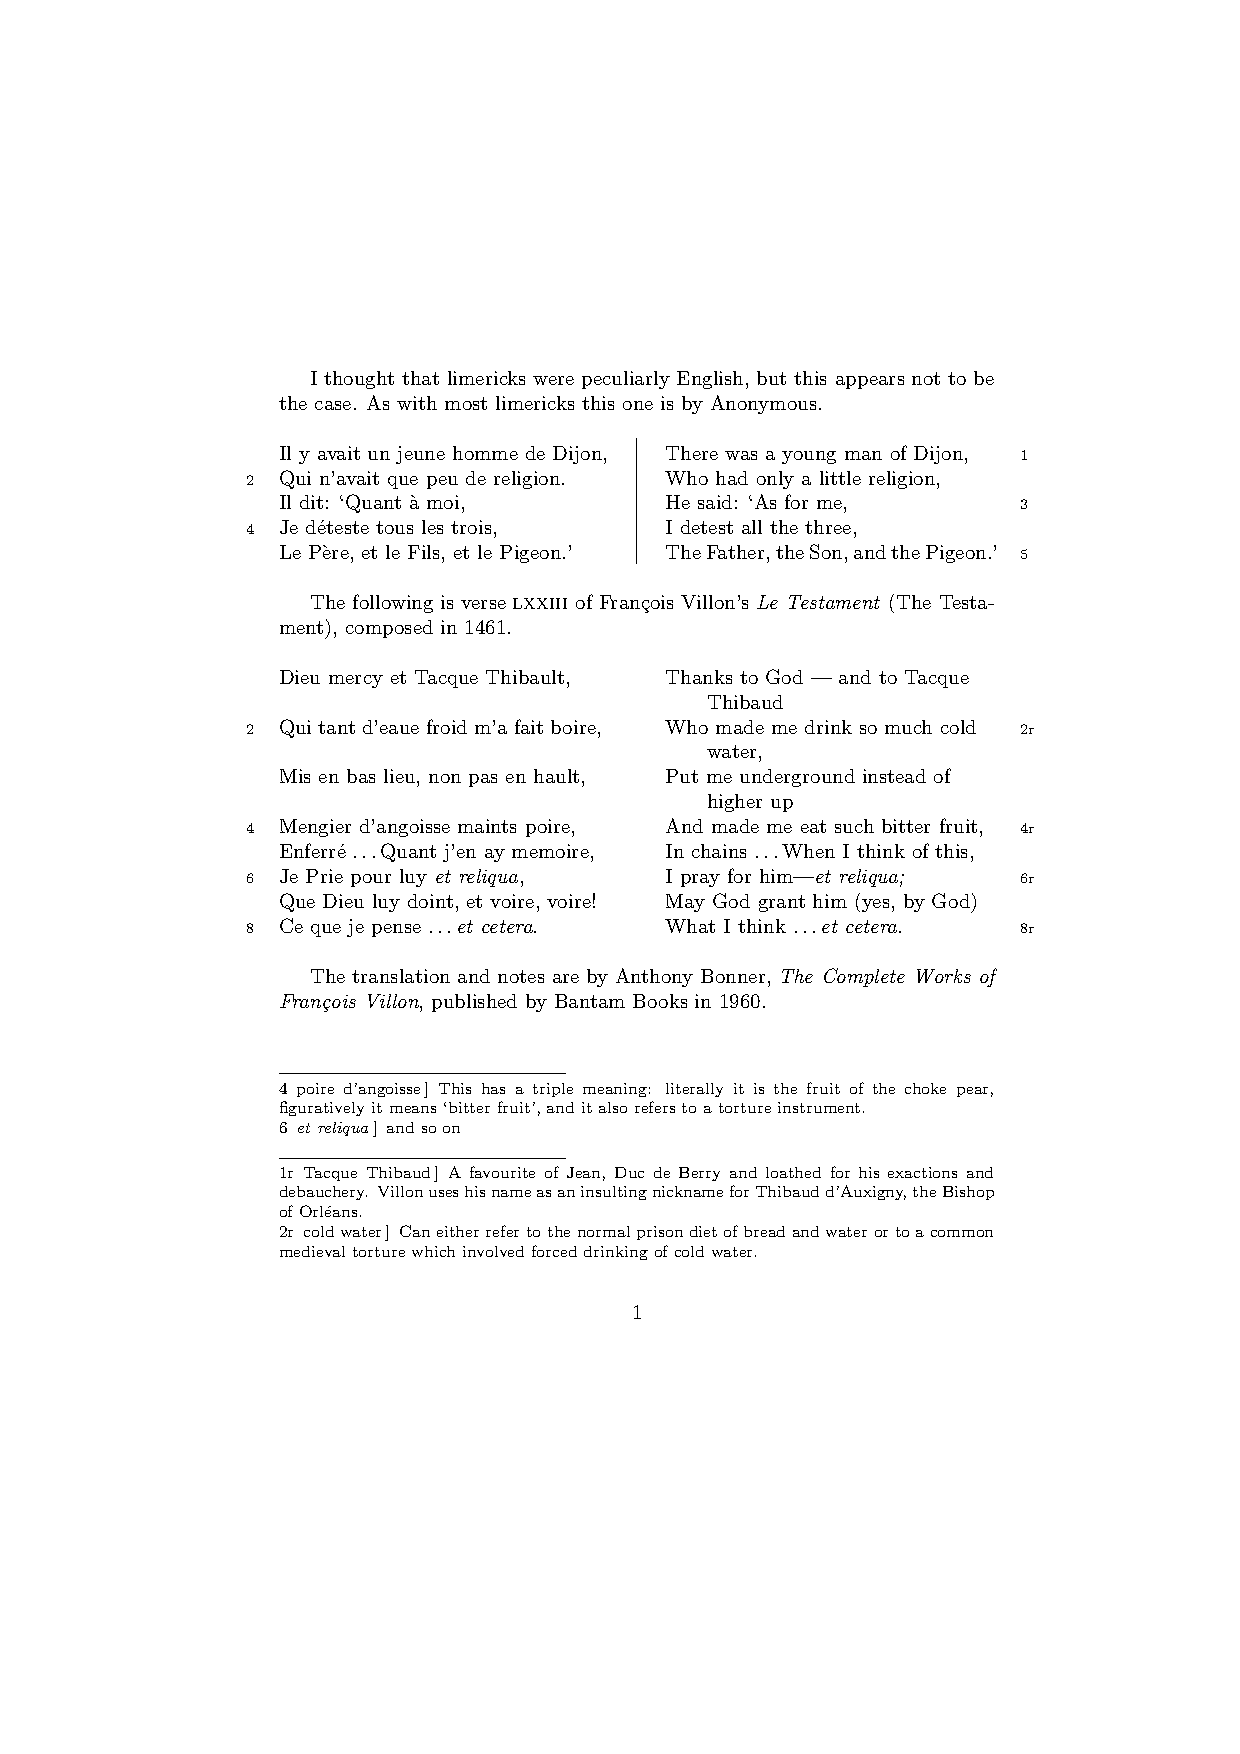
\includegraphics{villon}
% \caption{Output from \file{villon.tex}.}
% \label{villon-out}
% \end{figure}
%
% \begin{figure}[p]
% \centering
% 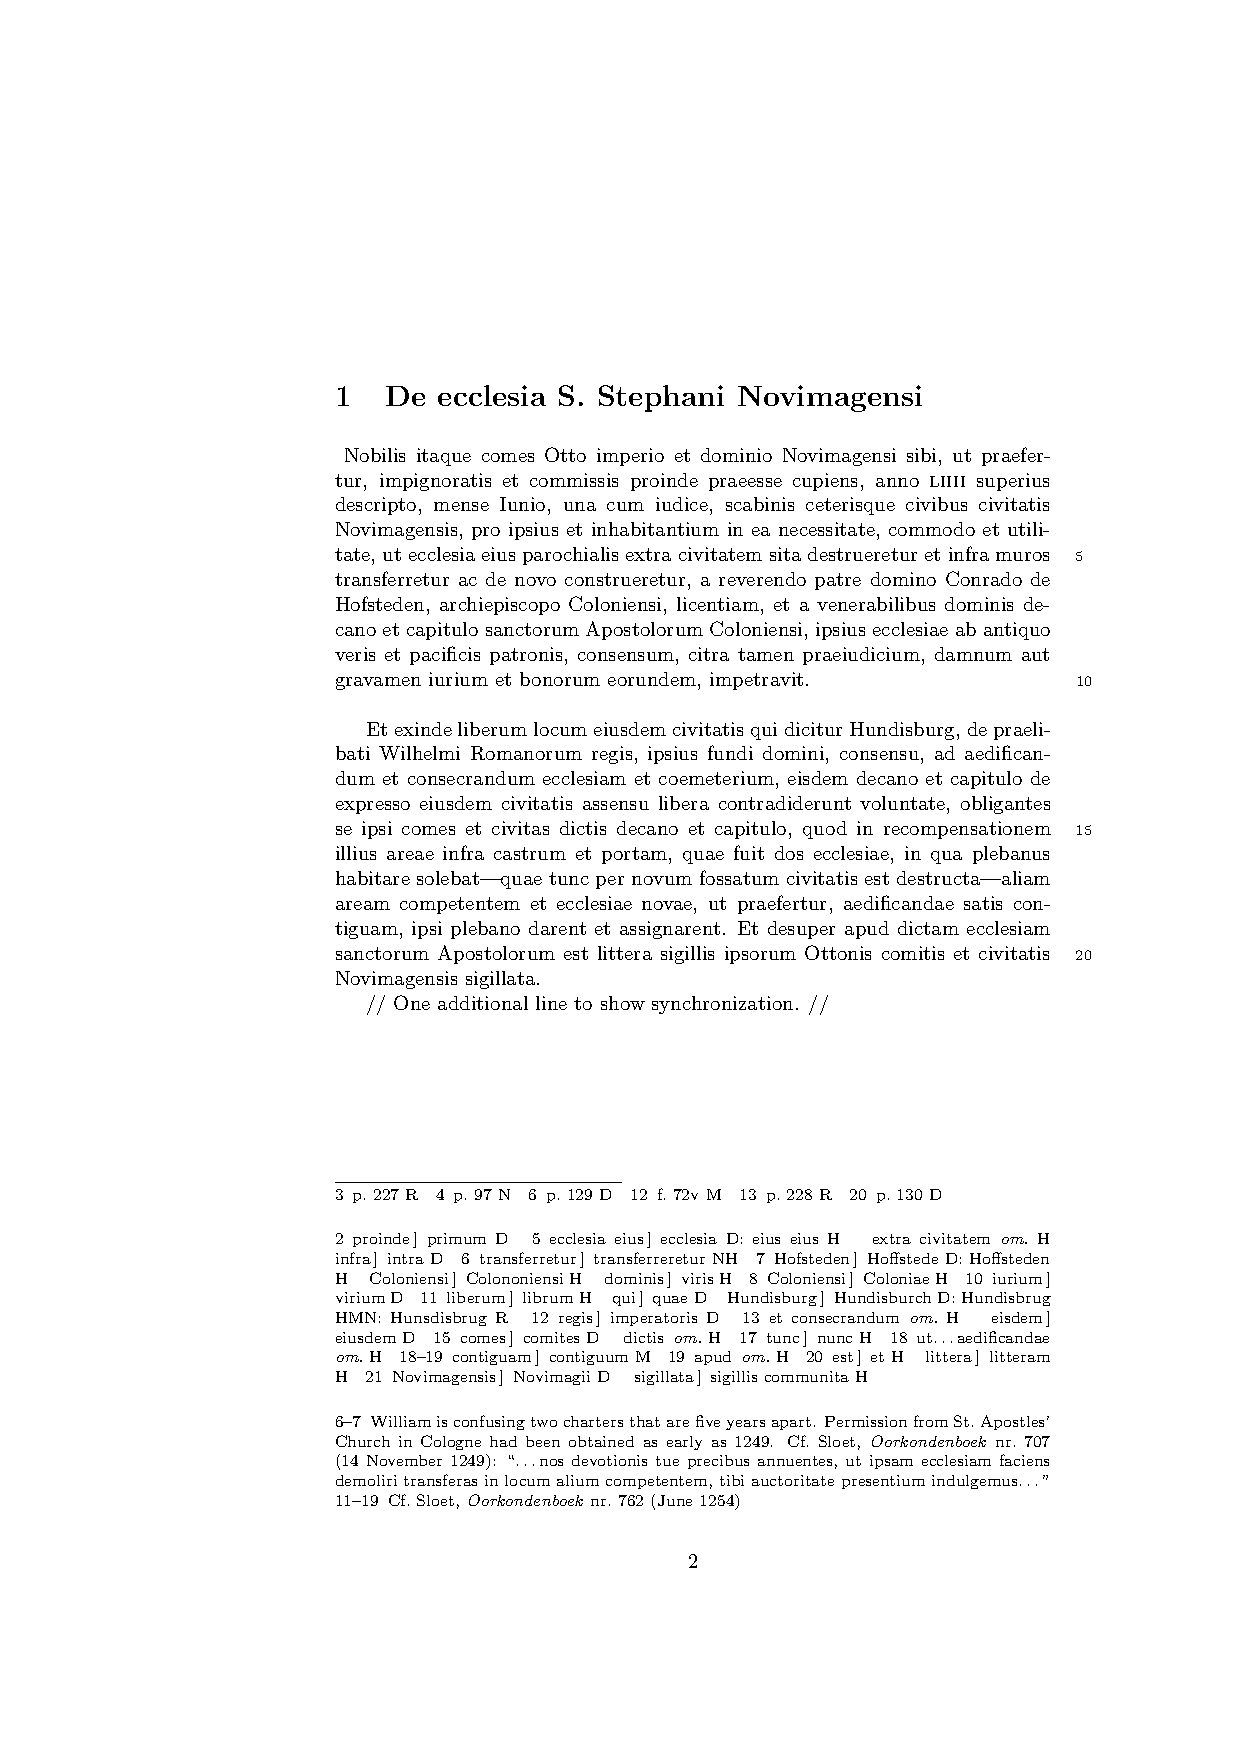
\includegraphics{djd17novL}
% \caption{Left page output from \file{djd17nov.tex}.}
% \label{djdL-out}
% \end{figure}
%
% \begin{figure}[p]
% \centering
% 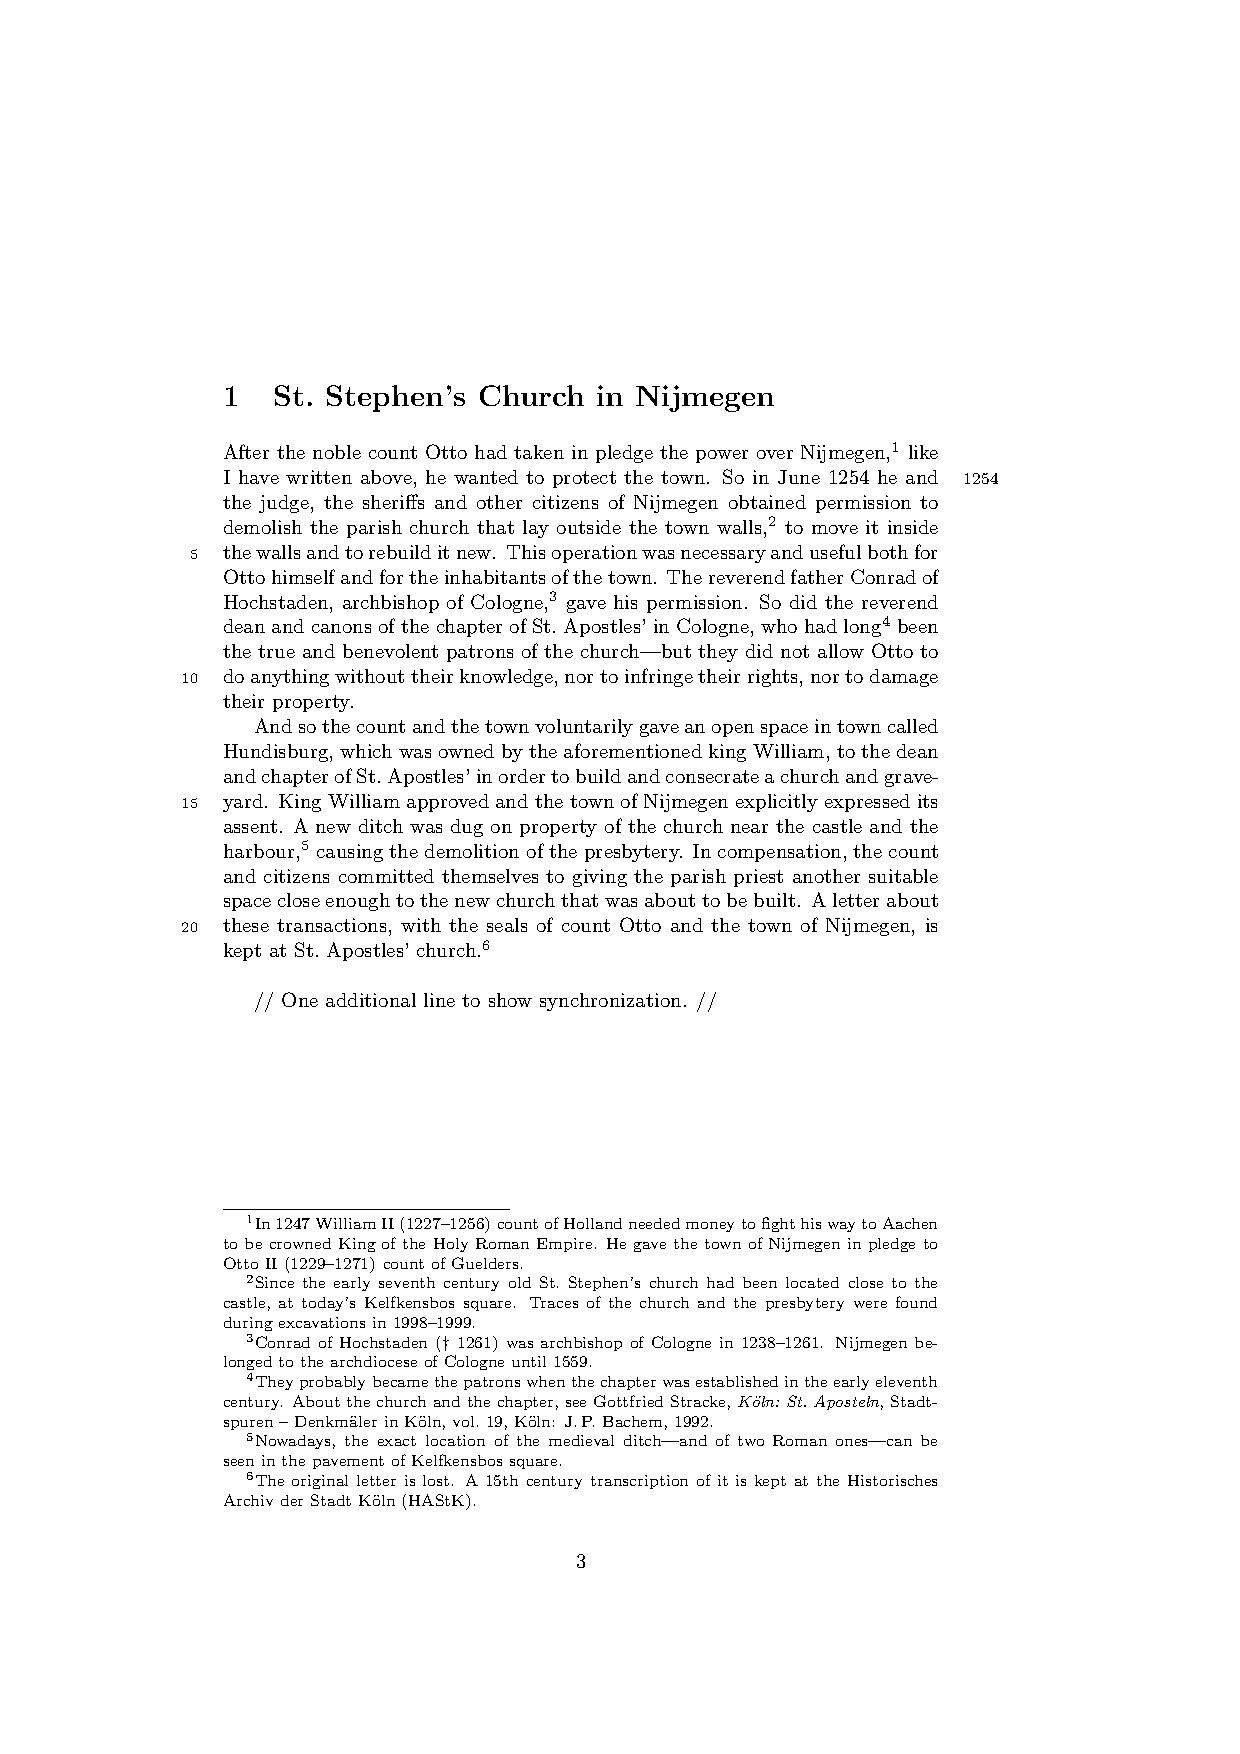
\includegraphics{djd17novR}
% \caption{Right page output from \file{djd17nov.tex}.}
% \label{djdR-out}
% \end{figure}
%
% \begin{figure}[p]
% \centering
% 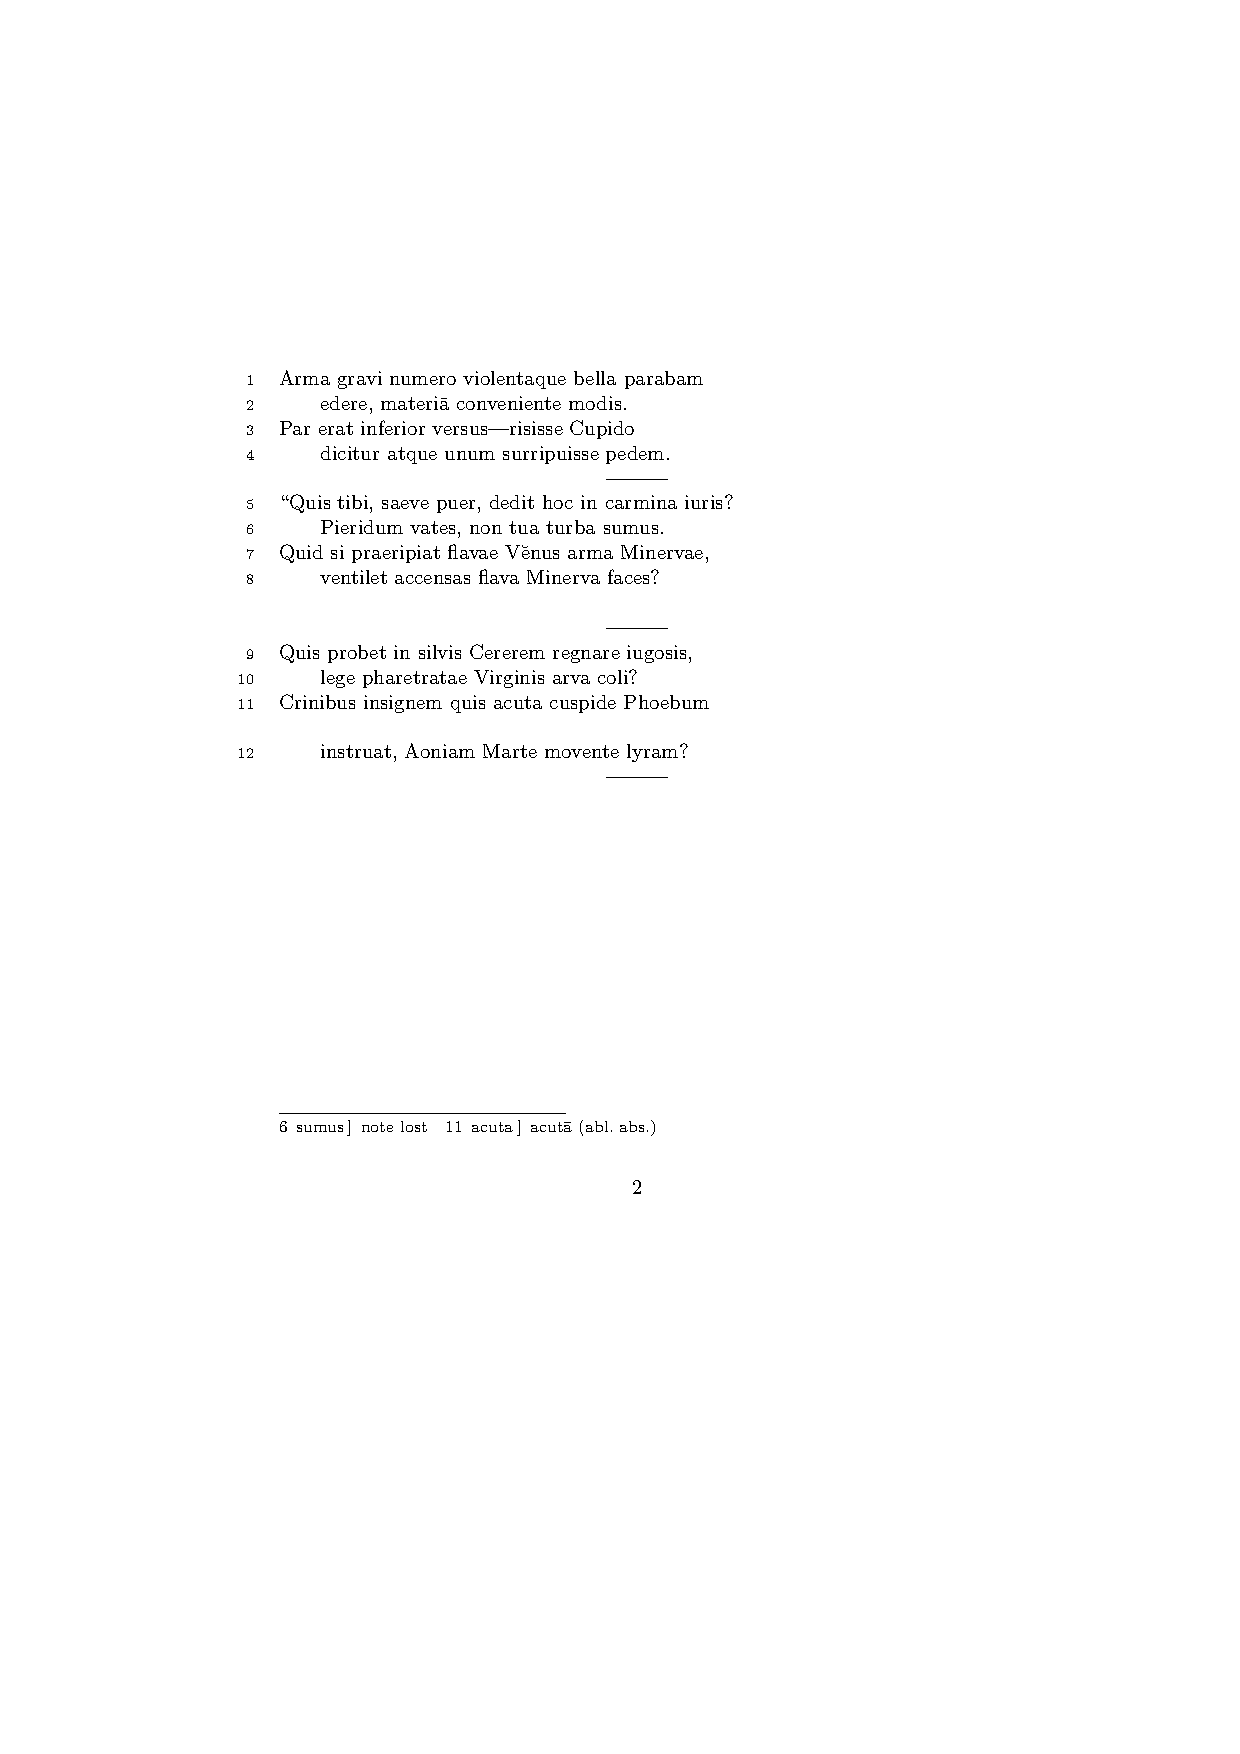
\includegraphics{djdpoems1}
% \caption{First left page output from \file{djdpoems.tex}.}
% \label{djdp1-out}
% \end{figure}
%
% \begin{figure}[p]
% \centering
% 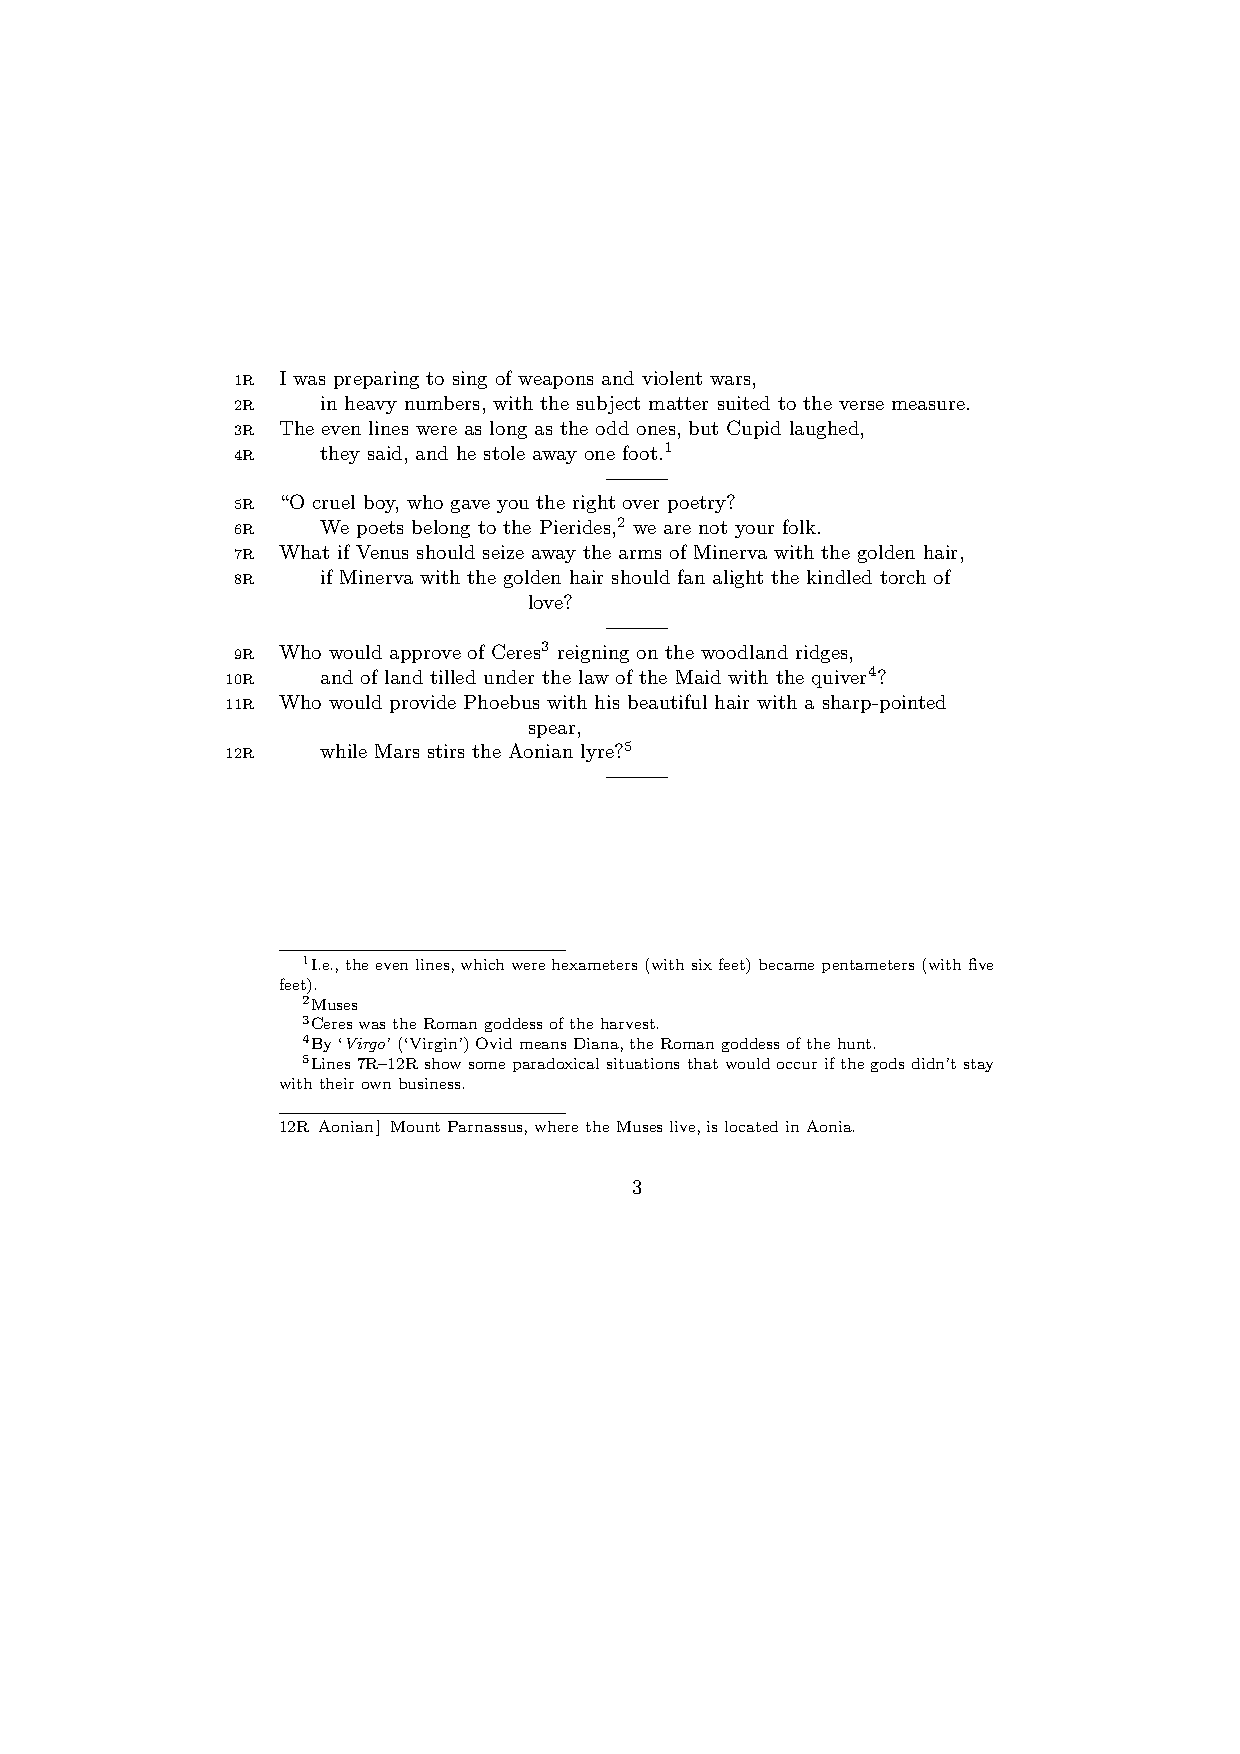
\includegraphics{djdpoems2}
% \caption{First right page output from \file{djdpoems.tex}.}
% \label{djdp2-out}
% \end{figure}
%
% \begin{figure}[p]
% \centering
% 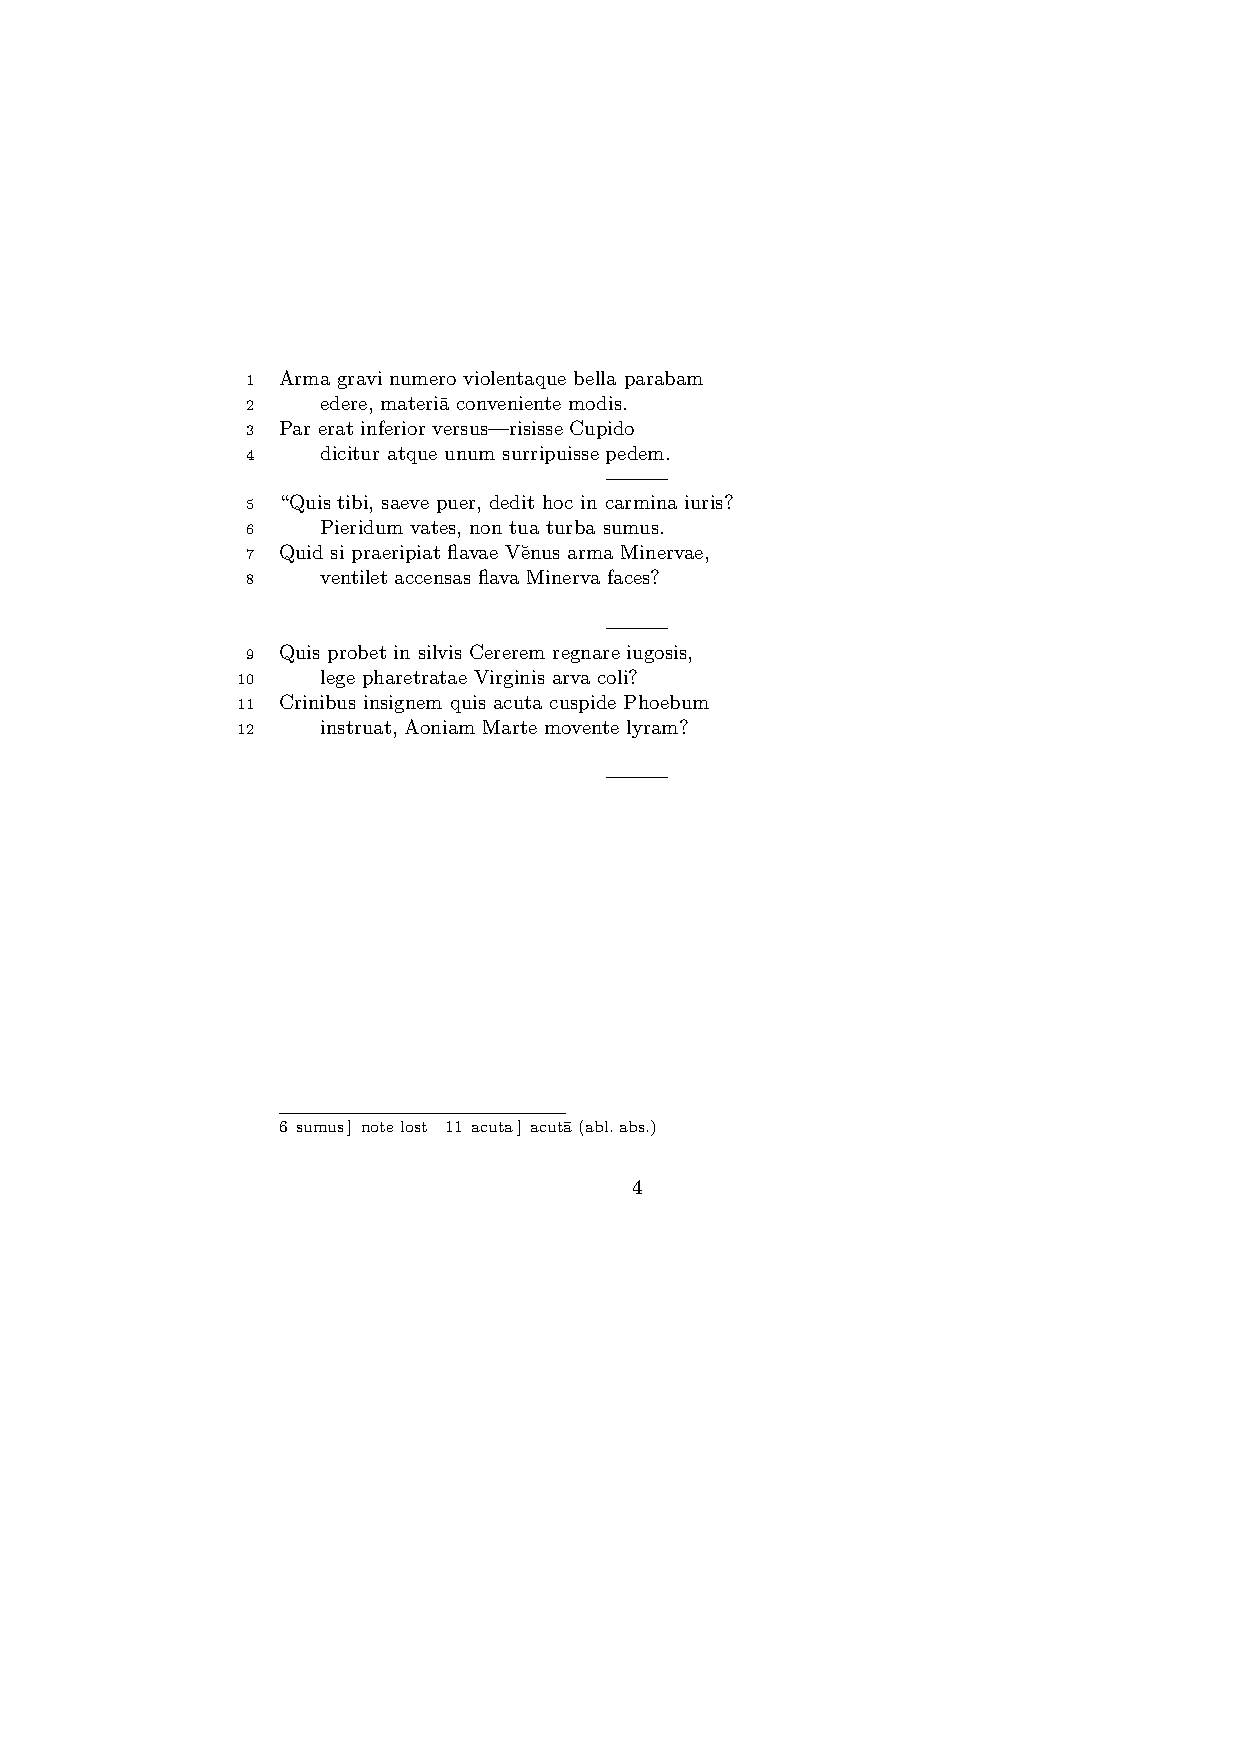
\includegraphics{djdpoems3}
% \caption{Second left page output from \file{djdpoems.tex}.}
% \label{djdp3-out}
% \end{figure}
%
% \begin{figure}[p]
% \centering
% 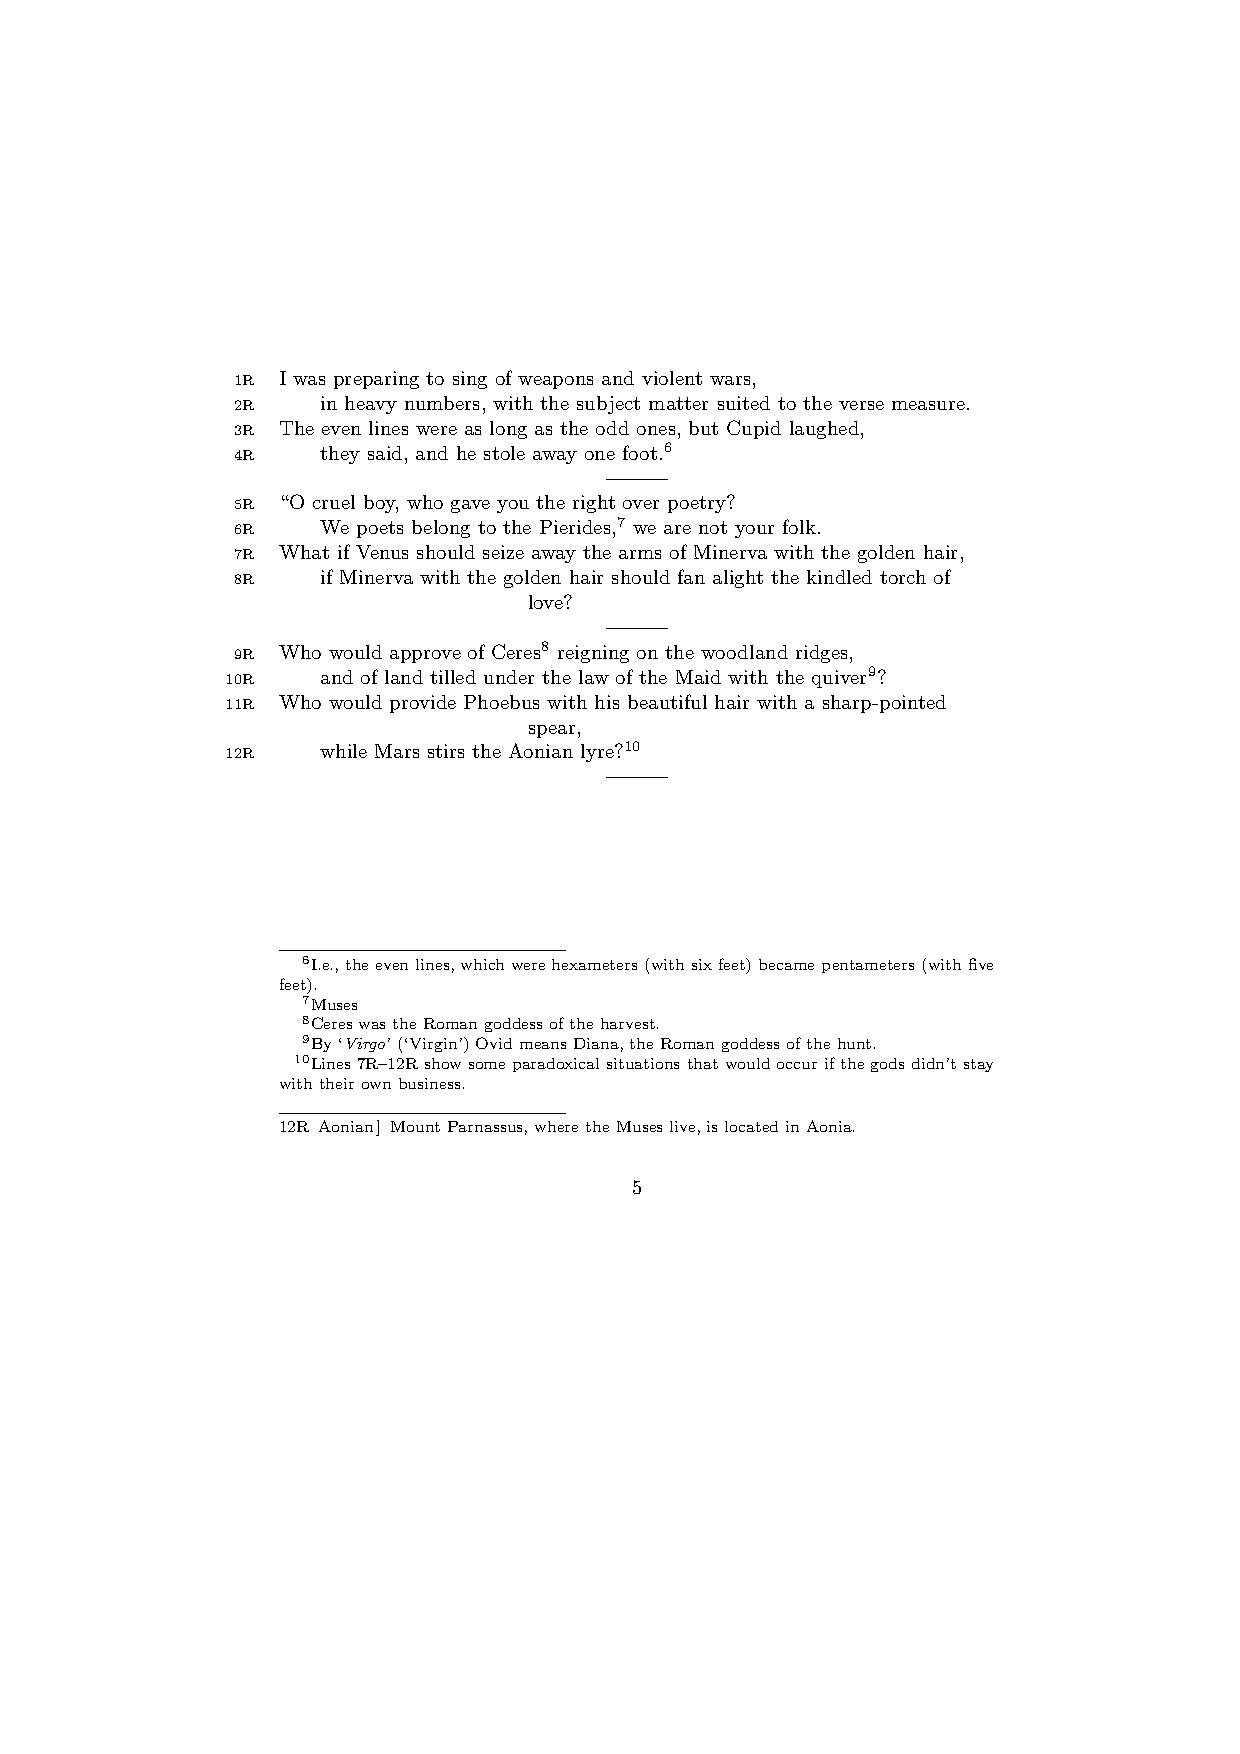
\includegraphics{djdpoems4}
% \caption{Second right page output from \file{djdpoems.tex}.}
% \label{djdp4-out}
% \end{figure}
%
%
%
% \clearpage
%
% \subsection{Parallel column example}\label{example:villon}
%
% This made-up example, \file{villon.tex}, is included to show 
% parallel columns and how they can be interspersed in regular text.
% The verses are set using the \cs{stanza} construct, where each 
% verse line is a chunk.
% The code is given below and the result is shown in Figure~\ref{villon-out}.
%
% \medskip
% \hrule
% \medskip
%    \begin{macrocode}
%<*villon>
%%% villon.tex Example parallel columns
\documentclass{article}
\addtolength{\textheight}{-10\baselineskip}
\usepackage{ledmac,ledpar}
%% Use r instead of R to flag right text line numbers
\renewcommand{\Rlineflag}{r}
%% Use the flag in the notes
\let\oldBfootfmt\Bfootfmt
\renewcommand{\Bfootfmt}[3]{%
  \let\printlines\printlinesR
  \oldBfootfmt{#1}{#2}{#3}}
\begin{document}

I thought that limericks were peculiarly English, but this appears not
to be the case. As with most limericks this one is by Anonymous.

\vspace*{\baselineskip}

\begin{pairs}
%% no indentation
\setstanzaindents{0,0,0,0,0,0,0,0,0}
%% no number flag
\renewcommand{\Rlineflag}{}
%% draw a rule and widen the columns
\setlength{\columnrulewidth}{0.4pt}
\setlength{\Lcolwidth}{0.46\textwidth}
\setlength{\Rcolwidth}{\Lcolwidth}

\begin{Leftside}
%% set left text line numbering sequence
\firstlinenum{2}
\linenumincrement{2}
\linenummargin{left}
\beginnumbering
\stanza
Il y avait un jeune homme de Dijon, &
Qui n'avait que peu de religion. &
Il dit: `Quant \`{a} moi, &
Je d\'{e}teste tous les trois, &
Le P\`{e}re, et le Fils, et le Pigeon.' \&
\endnumbering
\end{Leftside}

\begin{Rightside}
%% different right text line numbering sequence
\firstlinenum{1}
\linenumincrement{2}
\linenummargin{right}
\beginnumbering
\stanza
There was a young man of Dijon, &
Who had only a little religion, &
He said: `As for me, & 
I detest all the three, &
The Father, the Son, and the Pigeon.' \&
\endnumbering
\end{Rightside}

\Columns
\end{pairs}

\vspace*{\baselineskip}

    The following is verse \textsc{lxxiii} of Fran\c{c}ois Villon's 
\textit{Le Testament} (The Testament), composed in 1461.

%% Allow for hanging indentation for long lines
\setstanzaindents{1,0,0,0,0,0,0,0,0}
%% Columns wider than the default
\setlength{\Lcolwidth}{0.46\textwidth}
\setlength{\Rcolwidth}{\Lcolwidth}
\vspace*{\baselineskip}

\begin{pairs}
\begin{Leftside}
\firstlinenum{2}
\linenumincrement{2}
\linenummargin{left}
\beginnumbering
\stanza
Dieu mercy et Tacque Thibault, &
Qui tant d'eaue froid m'a fait boire, &
Mis en bas lieu, non pas en hault, &
Mengier d'angoisse maints \edtext{poire}{\lemma{poire d'angoisse}%
  \Afootnote{This has a triple meaning: literally it is the fruit of the 
  choke pear,
  figuratively it means `bitter fruit', and it also refers to a torture
  instrument.}}, &
Enferr\'{e} \ldots Quant j'en ay memoire, &
Je Prie pour luy \edtext{\textit{et reliqua}}{\Afootnote{and so on}}, &
Que Dieu luy doint, et voire, voire! &
Ce que je pense \ldots \textit{et cetera}. \&
\endnumbering
\end{Leftside}

\begin{Rightside}
\firstlinenum{2}
\linenumincrement{2}
\linenummargin{right}
\beginnumbering
\stanza
Thanks to God --- and to \edtext{Tacque Thibaud}{%
  \Bfootnote{A favourite of Jean, Duc de Berry and loathed for his exactions
  and debauchery. Villon uses his name as an insulting nickname for
  Thibaud d'Auxigny, the Bishop of Orl\'{e}ans.}}  &
Who made me drink so much \edtext{cold water}{%
  \Bfootnote{Can either refer to the normal prison diet of bread and 
   water or to a common medieval torture which involved forced drinking 
   of cold water.}}, &
Put me underground instead of higher up &
And made me eat such bitter fruit, &
In chains \ldots When I think of this, &
I pray for him---\textit{et reliqua;} &
May God grant him (yes, by God) &
What I think \ldots \textit{et cetera}. \&
\endnumbering
\end{Rightside}

\Columns
\end{pairs}

\vspace*{\baselineskip}

    The translation and notes are by Anthony Bonner, 
\textit{The Complete Works of Fran\c{c}ois Villon}, published by 
Bantam Books in 1960.

\end{document}

%</villon>
%    \end{macrocode}
%
%
% \subsection{Example parallel facing pages} \label{example:djd17nov}
%
% This example, illustrated in Figures~\ref{djdL-out} and~\ref{djdR-out},
% was provided in November 2004 by Dirk-Jan Dekker\index{Dekker, Dirk-Jan}
% of the Department of Medieval History at Radboud University, Nijmegen.
%
% \medskip
% \hrule
% \medskip
%
%    \begin{macrocode}
%<*djd17nov>
%%% This is djd17nov.tex, a sample critical text edition
%%% written in LaTeX2e with the ledmac and ledpar packages.
%%% (c) 2003--2004 by Dr. Dirk-Jan Dekker,
%%% Radboud University, Nijmegen (The Netherlands)
%%% (PRW) Modified slightly by PRW to fit the ledpar manual

\documentclass[10pt, letterpaper, twoside]{article}
\usepackage[latin,english]{babel}
\usepackage{makeidx}
\usepackage{ledmac,ledpar}
\lineation{section}
\linenummargin{inner}
\sidenotemargin{outer}

\makeindex

\renewcommand{\notenumfont}{\footnotesize}
\newcommand{\notetextfont}{\footnotesize}

%\let\Afootnoterule=\relax
\let\Bfootnoterule=\relax
\let\Cfootnoterule=\relax

\addtolength{\skip\Afootins}{1.5mm}
%\addtolength{\skip\Bfootins}{1.5mm}
%\addtolength{\skip\Cfootins}{1.5mm}

\makeatletter

\renewcommand*{\para@vfootnote}[2]{%
  \insert\csname #1footins\endcsname
  \bgroup
    \notefontsetup
    \interlinepenalty=\interfootnotelinepenalty
    \floatingpenalty=\@MM
    \splittopskip=\ht\strutbox \splitmaxdepth=\dp\strutbox
    \leftskip=\z@skip \rightskip=\z@skip
    \l@dparsefootspec #2\ledplinenumtrue%                  new from here
    \ifnum\@nameuse{previous@#1@number}=\l@dparsedstartline\relax
      \ledplinenumfalse
     \fi
     \ifnum\previous@page=\l@dparsedstartpage\relax
     \else \ledplinenumtrue \fi
     \ifnum\l@dparsedstartline=\l@dparsedendline\relax
     \else \ledplinenumtrue \fi
     \expandafter\xdef\csname previous@#1@number\endcsname{\l@dparsedstartline}%
     \xdef\previous@page{\l@dparsedstartpage}%            to here
     \setbox0=\vbox{\hsize=\maxdimen
       \noindent\csname #1footfmt\endcsname#2}%
      \setbox0=\hbox{\unvxh0}%
      \dp0=0pt
      \ht0=\csname #1footfudgefactor\endcsname\wd0
      \box0
      \penalty0
  \egroup
}

\newcommand*{\previous@A@number}{-1}
\newcommand*{\previous@B@number}{-1}
\newcommand*{\previous@C@number}{-1}
\newcommand*{\previous@page}{-1}

\newcommand{\abb}[1]{#1%
        \let\rbracket\nobrak\relax}
\newcommand{\nobrak}{\textnormal{}}
\newcommand{\morenoexpands}{%
        \let\abb=0%
}

\newcommand{\Aparafootfmt}[3]{%
  \ledsetnormalparstuff
  \scriptsize
  \notenumfont\printlines#1|\enspace
%  \lemmafont#1|#2\enskip
  \notetextfont
  #3\penalty-10\hskip 1em plus 4em minus.4em\relax}
        
\newcommand{\Bparafootfmt}[3]{%
  \ledsetnormalparstuff
  \scriptsize
  \notenumfont\printlines#1|%
  \ifledplinenum
  	\enspace
  \else
  	{\hskip 0em plus 0em minus .3em}%
  \fi
  \select@lemmafont#1|#2\rbracket\enskip
  \notetextfont
  #3\penalty-10\hskip 1em plus 4em minus.4em\relax }
       
\newcommand{\Cparafootfmt}[3]{%
  \ledsetnormalparstuff
  \scriptsize
  \notenumfont\printlines#1|\enspace
%  \lemmafont#1|#2\enskip
  \notetextfont
  #3\penalty-10\hskip 1em plus 4em minus.4em\relax}

\makeatother

\footparagraph{A}
\footparagraph{B}
\footparagraph{C}

\let\Afootfmt=\Aparafootfmt
\let\Bfootfmt=\Bparafootfmt
\let\Cfootfmt=\Cparafootfmt

\renewcommand*{\Rlineflag}{}

\emergencystretch40pt

\author{Guillelmus de Berchen}
\title{Chronicon Geldriae}
\date{}
\hyphenation{archi-epi-sco-po Huns-dis-brug li-be-ra No-vi-ma-gen-si}
\begin{document}
\begin{pages}
\begin{Leftside}
\beginnumbering\pstart
\selectlanguage{latin}
\section{De ecclesia S. Stephani Novimagensi}

\noindent\setline{1}
Nobilis itaque comes Otto\protect\edindex{Otto II of Guelders} 
imperio et dominio Novimagensi sibi, ut praefertur, impignoratis 
et commissis 
\edtext{proinde}{\Bfootnote{primum D}} praeesse cupiens, anno 
\textsc{liiii} superius descripto, mense 
Iu\edtext{}{\Afootnote{p.\ 227~R}}nio, una cum iudice, scabinis ceterisque 
civibus civitatis Novimagensis, pro ipsius et inhabitantium in ea 
necessitate,\edtext{}{\Afootnote{p.\ 97~N}} commodo et utilitate, 
ut \edtext{ecclesia eius}{\Bfootnote{ecclesia D: eius eius H}} parochialis 
\edtext{\abb{extra civitatem}}{\Bfootnote{\textit{om.}~H}} sita 
destrueretur et \edtext{infra}{\Bfootnote{intra D}} muros 
\edtext{transfer\edtext{}{\Afootnote{p.\ 129~D}}retur}%
{\Bfootnote{transferreretur NH}} 
ac de novo construeretur, 
\edtext{a reverendo patre domino 
Conrado\protect\edindex{Conrad of Hochstaden} de 
\edtext{Hofsteden}{\Bfootnote{Hoffstede D: Hoffsteden H}}, archiepiscopo 
\edtext{Coloniensi}{\Bfootnote{Colononiensi H}}, licentiam}%
{\Cfootnote{William is confusing two charters that are five years 
apart. Permission from St.\ Apostles' Church in Cologne had been 
obtained as early as 1249. Cf.\ 
Sloet\protect\index{Sloet van de Beele, L.A.J.W.}, 
\textit{Oorkondenboek} nr.\ 707 (14 November 1249): 
``\ldots{}nos devotionis tue precibus annuentes, ut ipsam ecclesiam 
faciens demoliri transferas in locum alium competentem, tibi 
auctoritate presentium indulgemus\ldots''}}, et a venerabilibus 
\edtext{dominis}{\Bfootnote{viris H}} decano et capitulo sanctorum 
Apostolorum\protect\edindex{St. Apostles' (Cologne)} 
\edtext{Coloniensi}{\Bfootnote{Coloniae H}}, ipsius ecclesiae ab 
antiquo veris et pacificis patronis, consensum, citra tamen 
praeiudicium, damnum aut gravamen \edtext{iurium}{\Bfootnote{virium D}} 
et bonorum eorundem, impetravit.
\pend

\pstart
\edtext{Et exinde \edtext{liberum}{\Bfootnote{librum H}} 
locum eiusdem civitatis 
\edtext{qui}{\Bfootnote{quae D}} dicitur 
\edtext{Hundisburg}{\Bfootnote{Hundisburch D: Hundisbrug HMN: 
Hunsdisbrug R}}\protect\edindex{Hundisburg}, 
de praelibati Wilhelmi\protect\edindex{William II of Holland} Romanorum 
\edtext{regis}{\Bfootnote{imperatoris D}}, ipsius fundi 
do\edtext{}{\Afootnote{f.\ 72v~M}}mini, consensu, ad aedificandum 
\edtext{\abb{et consecrandum}}{\Bfootnote{\textit{om.}\ H}} 
ecclesi\edtext{}{\Afootnote{p.\ 228~R}}am et coemeterium, 
\edtext{eisdem}{\Bfootnote{eiusdem D}} decano et capitulo de expresso 
eiusdem civitatis assensu libera contradiderunt voluntate, obligantes 
se ipsi \edtext{comes}{\Bfootnote{comites D}} et civitas 
\edtext{\abb{dictis}}{\Bfootnote{\textit{om.}\ H}} decano et capitulo, 
quod in recompensationem illius areae infra castrum et portam, quae 
fuit dos ecclesiae, in qua plebanus habitare solebat---quae 
\edtext{tunc}{\Bfootnote{nunc H}} per novum fossatum civitatis est 
destructa---aliam aream competentem et ecclesiae novae, 
\edtext{ut praefertur, aedificandae}{%
\lemma{\abb{ut\ldots aedificandae}}\Bfootnote{\textit{om.}\ H}} satis 
\edtext{contiguam}{\Bfootnote{contiguum M}}, ipsi plebano darent et 
assignarent.}{\Cfootnote{Cf.\ Sloet, \textit{Oorkondenboek} nr.\ 762 
(June 1254)}} Et desuper 
\edtext{\abb{apud}}{\Bfootnote{\textit{om.}\ H}} dictam ecclesiam 
sanctorum Apostolorum \edtext{est}{\Bfootnote{et H}} 
\edtext{littera}{\Bfootnote{litteram H}} sigillis ipsorum 
Ottonis\edtext{}{\Afootnote{p.\ 130~D}} comitis et civitatis 
\edtext{Novimagensis}{\Bfootnote{Novimagii D}} 
\edtext{sigillata}{\Bfootnote{sigillis communita H}}.
\pend

\pstart
 // One additional line to show synchronization. //
\pend
\endnumbering
\end{Leftside}

\begin{Rightside}
\sidenotemargin{right}\selectlanguage{english}
\beginnumbering
\pstart
\addtocounter{section}{-1}%
\leavevmode\section{St.\ Stephen's Church in Nijmegen}

\noindent\setline{1}%
After the noble count Otto had taken in pledge the power over 
Nijmegen,\footnote{In 1247 William II\protect\index{William II of Holland} 
(1227--1256) count of Holland needed money to fight his way to 
Aachen\protect\index{Aachen} to be crowned King of the Holy Roman 
Empire. He gave the town of Nijmegen in pledge to Otto 
II\protect\index{Otto II of Guelders} (1229--1271) count of Guelders.} 
like I have written above, he wanted to protect the town. So in June 
1254\ledsidenote{1254} he and the judge, the sheriffs and other 
citizens of Nijmegen obtained permission to demolish the parish 
church that lay outside the town walls,\footnote{Since the early 
seventh century old St.\ Stephen's church had been located close 
to the castle, at today's 
Kelfkensbos\protect\index{Kelfkensbos (Nijmegen)} square. 
Traces of the church and the presbytery were found during excavations 
in 1998--1999.} to move it inside the walls and to rebuild it new. 
This operation was necessary and useful both for Otto himself and 
for the inhabitants of the town. The reverend father Conrad of 
Hochstaden, archbishop of 
Cologne,\footnote{Conrad of Hochstaden ({\textdagger} 1261) was 
archbishop of Cologne in 1238--1261. Nijmegen belonged to the 
archdiocese of Cologne until 1559.} gave his permission. So did the 
reverend dean and canons of the chapter of St.\ 
Apostles'\protect\index{St. Apostles' (Cologne)} in Cologne, who had 
long\footnote{They probably became the patrons when the chapter was 
established in the early eleventh century. About the church and the 
chapter, see Gottfried Stracke\protect\index{Stracke, G.}, 
\textit{K\"{o}ln:\ St.\ Aposteln}, Stadtspuren -- Denkm\"{a}ler in 
K\"{o}ln, vol.\ 19, K\"{o}ln: J.\,P.\ Bachem, 1992.} been the true 
and benevolent patrons of the church---but they did not allow Otto 
to do anything without their knowledge, nor to infringe their rights, 
nor to damage their property.
\pend

\pstart 
And so the count and the town voluntarily gave an open space in town 
called Hundisburg, which was owned by the aforementioned king William, 
to the dean and chapter of St.\ Apostles' in order to build and 
consecrate a church and graveyard. King William approved and the 
town of Nijmegen explicitly expressed its assent. A new ditch was dug 
on property of the church near the castle and the 
harbour,\footnote{Nowadays, the exact location of the medieval 
ditch---and of two Roman ones---can be seen in the pavement of 
Kelfkensbos\protect\index{Kelfkensbos (Nijmegen)} square.} causing 
the demolition of the presbytery. In compensation, the count and 
citizens committed themselves to giving the parish priest another 
suitable space close enough to the new church that was about to be 
built. A letter about these transactions, with the seals of count 
Otto and the town of Nijmegen, is kept at St.\ Apostles' 
church.\footnote{The original letter is lost. A 15th century 
transcription of it is kept at the Historisches Archiv der 
Stadt K\"{o}ln (HAStK).}
\pend

\pstart 
// One additional line to show synchronization. //
\pend
\endnumbering
\end{Rightside}
\Pages
\end{pages}

%%%%%%%%%%%%%%%%%%%%%%%%%%%
\printindex
\end{document}
%%%%%%%%%%%%%%%%%%

%</djd17nov>
%    \end{macrocode}
%
% \medskip
% \hrule
%
% \subsection{Example poetry on parallel facing pages} \label{example:djdpoems}
%
% This example, illustrated in Figures~\ref{djdp1-out} to~\ref{djdp4-out},
% was originally provided in November 2004 by 
% Dirk-Jan Dekker\index{Dekker, Dirk-Jan} for an earlier version of \Ledpar.
% I have updated it, and also extended it to show the difference between
% the \cs{stanza} command and the \verb?astanza? environment. \cs{stanza}
% is used for the first pair of pages and \verb?astanza? for the second
% pair. Note the
% definition of \cs{endstanzaextra} to give a short line after each stanza.
%
% \medskip
% \hrule
% \medskip
%
%    \begin{macrocode}
%<*djdpoems>
%%% djdpoems.tex  example parallel verses on facing pages
\documentclass{article}
\usepackage{ledmac,ledpar}
\addtolength{\textheight}{-15\baselineskip}

\maxchunks{24} % default value = 10
\setstanzaindents{6,0,1,0,1}

\newcommand{\longdash}{---------}

\footparagraph{A} % for left pages
\footparagraph{B} % for right pages
\firstlinenum{1}
\linenumincrement{1}

\let\oldBfootfmt\Bfootfmt
\renewcommand{\Bfootfmt}[3]{%
   \let\printlines\printlinesR
   \oldBfootfmt{#1}{#2}{#3}}
   
\begin{document}

\newcommand{\interstanza}{\pstart\centering\longdash\skipnumbering\pend}

\begin{pages}
\begin{Leftside}
\def\endstanzaextra{\interstanza}
\beginnumbering

\stanza
Arma gravi numero violentaque bella parabam &
 edere, materi\={a} conveniente modis. &
Par erat inferior versus---risisse Cupido &
 dicitur atque unum surripuisse pedem. \&

\stanza
``Quis tibi, saeve puer, dedit hoc in carmina iuris? &
 Pieridum vates, non tua turba \edtext{sumus}{\Afootnote{note lost}}. &
Quid si praeripiat flavae V\u{e}nus arma Minervae, &
 ventilet accensas flava Minerva faces? \&

\stanza
Quis probet in silvis Cererem regnare iugosis, &
 lege pharetratae Virginis arva coli? &
Crinibus insignem quis \edtext{acuta}{\Afootnote{acut\={a} (abl.\ abs.)}} 
cuspide Phoebum &
 instruat, Aoniam Marte movente lyram? \&
\endnumbering
\end{Leftside}

\begin{Rightside}
\def\endstanzaextra{\interstanza}
\beginnumbering
\firstlinenum{1}
\linenumincrement{1}
\setstanzaindents{6,0,1,0,1,0}

\stanza
I was preparing to sing of weapons and violent wars, &
in heavy numbers, with the subject matter suited to the verse measure. &
The even lines were as long as the odd ones, but Cupid laughed, &
they said, and he stole away one foot.\footnote{I.e., the even lines, 
which were hexameters (with six feet) became pentameters 
(with five feet).} \&

\stanza
``O cruel boy, who gave you the right over poetry? &
We poets belong to the Pierides,\footnote{Muses} we are not your folk. &
\edlabel{beginparadox}What if Venus should seize away the arms of 
Minerva with the golden hair, &
 if Minerva with the golden hair should fan alight the kindled torch 
of love? \&
 
\stanza
Who would approve of Ceres\footnote{Ceres was the Roman goddess of 
the harvest.} reigning on the woodland ridges, &
 and of land tilled under the law of the Maid with the 
quiver\footnote{By `\textit{Virgo}' (`Virgin') Ovid means Diana, the 
Roman goddess of the hunt.}? &
Who would provide Phoebus with his beautiful hair with a sharp-pointed 
spear, &
 while Mars stirs the \edtext{Aonian}{\Bfootnote{Mount Parnassus, 
where the Muses live, is located in Aonia.}} 
lyre?\edlabel{endparadox}\footnote{Lines 
\xlineref{beginparadox}--\xlineref{endparadox} show some paradoxical 
situations that would occur if the gods didn't stay with their own 
business.} \&
\endnumbering
\end{Rightside}

\Pages
\end{pages}

\begin{pages}
\begin{Leftside}
\def\endstanzaextra{\interstanza}
\beginnumbering

\begin{astanza}
Arma gravi numero violentaque bella parabam &
 edere, materi\={a} conveniente modis. &
Par erat inferior versus---risisse Cupido &
 dicitur atque unum surripuisse pedem. \&
\end{astanza}

\begin{astanza}
``Quis tibi, saeve puer, dedit hoc in carmina iuris? &
 Pieridum vates, non tua turba \edtext{sumus}{\Afootnote{note lost}}. &
Quid si praeripiat flavae V\u{e}nus arma Minervae, &
 ventilet accensas flava Minerva faces? \&
\end{astanza}

\begin{astanza}
Quis probet in silvis Cererem regnare iugosis, &
 lege pharetratae Virginis arva coli? &
Crinibus insignem quis \edtext{acuta}{\Afootnote{acut\={a} (abl.\ abs.)}} 
cuspide Phoebum &
 instruat, Aoniam Marte movente lyram? \&
\end{astanza}

\endnumbering
\end{Leftside}

\begin{Rightside}
\def\endstanzaextra{\interstanza}
\beginnumbering
\firstlinenum{1}
\linenumincrement{1}
\setstanzaindents{6,0,1,0,1,0}

\begin{astanza}
I was preparing to sing of weapons and violent wars, &
in heavy numbers, with the subject matter suited to the verse measure. &
The even lines were as long as the odd ones, but Cupid laughed, &
they said, and he stole away one foot.\footnote{I.e., the even lines, 
which were hexameters (with six feet) became pentameters 
(with five feet).} \&
\end{astanza}

\begin{astanza}
``O cruel boy, who gave you the right over poetry? &
We poets belong to the Pierides,\footnote{Muses} we are not your folk. &
\edlabel{beginparadox}What if Venus should seize away the arms of 
Minerva with the golden hair, &
 if Minerva with the golden hair should fan alight the kindled torch 
of love? \&
\end{astanza}
 
\begin{astanza}
Who would approve of Ceres\footnote{Ceres was the Roman goddess of the 
harvest.} reigning on the woodland ridges, &
 and of land tilled under the law of the Maid with the 
quiver\footnote{By `\textit{Virgo}' (`Virgin') Ovid means Diana, 
the Roman goddess of the hunt.}? &
Who would provide Phoebus with his beautiful hair with a sharp-pointed 
spear, &
 while Mars stirs the \edtext{Aonian}{\Bfootnote{Mount Parnassus, where 
the Muses live, is located in Aonia.}} 
lyre?\edlabel{endparadox}\footnote{Lines 
\xlineref{beginparadox}--\xlineref{endparadox} show some paradoxical 
situations that would occur if the gods didn't stay with their 
own business.} \&
\end{astanza}

\endnumbering
\end{Rightside}

\Pages
\end{pages}

\end{document}

%</djdpoems>
%    \end{macrocode}
%
% \medskip
% \hrule
%
% \clearpage
%
% \bibliographystyle{alpha}
% \begin{thebibliography}{WWW99}
% \addcontentsline{toc}{section}{References}
% \bibitem[LW90]{EDMACTUG}
% John Lavagnino and Dominik Wujastyk.
% \newblock `An overview of \edmac: a \textsc{Plain} TeX format for
%            critical editions'.
% \newblock \emph{TUGboat}, \textbf{11}, 4, pp. 623--643, November 1990.
% \newblock (Code available from CTAN in
%            \texttt{macros/plain/contrib/edmac})
%
%
% \bibitem[Wil02]{MEMOIR}
% Peter Wilson.
% \newblock \emph{The \Lpack{memoir} class for configurable typesetting}.
% \newblock November 2002.
% \newblock (Available from CTAN in
%            \texttt{macros/latex/contrib/memoir})
%
% \bibitem[Wil04]{LEDMAC}
% Peter Wilson.
% \newblock \emph{\Lpack{ledmac} A presumptuous attempt to port
%            \Lpack{EDMAC},\Lpack{TABMAC} and \Lpack{EDSTANZA} to
%             LaTeX}.
% \newblock December 2004.
% \newblock (Available from CTAN in
%            \texttt{macros/latex/contrib/ledmac})
%
% \end{thebibliography}
%
% \Finale
% \section*{}
% \addcontentsline{toc}{section}{Index}
% \PrintIndex
%
% \section*{}
% \addcontentsline{toc}{section}{Change History}
% \PrintChanges
% \endinput
\endinput

%% \CharacterTabl
%%   Upper-case    \A\B\C\D\E\F\G\H\I\J\K\L\M\N\O\P\Q\R\S\T\U\V\W\X\Y\Z
%%   Lower-case    \a\b\c\d\e\f\g\h\i\j\k\l\m\n\o\p\q\r\s\t\u\v\w\x\y\z
%%   Digits        \0\1\2\3\4\5\6\7\8\9
%%   Exclamation   \!     Double quote  \"     Hash (number) \#
%%   Dollar        \$     Percent       \%     Ampersand     \&
%%   Acute accent  \'     Left paren    \(     Right paren   \)
%%   Asterisk      \*     Plus          \+     Comma         \,
%%   Minus         \-     Point         \.     Solidus       \/
%%   Colon         \:     Semicolon     \;     Less than     \<
%%   Equals        \=     Greater than  \>     Question mark \?
%%   Commercial at \@     Left bracket  \[     Backslash     \\
%%   Right bracket \]     Circumflex    \^     Underscore    \_
%%   Grave accent  \`     Left brace    \{     Vertical bar  \|
%%   Right brace   \}     Tilde         \~}
%%
